\chapter{Case Studies}
\label{ch:cases}

\textit{This chapter presents the results of three selected cases. We first apply the analytical frameworks established in Chapter \ref{ch:market} to characterize the market regimes in three cases and identify potential business opportunities for flexibility solutions. Thereafter, the quantitative methodology developed in Chapter \ref{ch:methodology} is used to estimate the market potential and profitability of selected flexibility solutions. It was found}

\section[Case selection: rationale and definition]{Case selection: rationale and definition%}
	\sectionmark{Case selction}}
\sectionmark{Case selction}
The goal of this thesis is to provide technology vendors, especially those who have an international ambition, a reference for strategic business planning regarding electricity flexibility solutions in different power market jurisdictions. This defines our rationale for case selections, explained below.

First, the case studies should be carried out in markets that have an significant impact on business on a global scale, so that results from case studies can be direct references to help technology vendors establish a global view of the business landscape for flexibility solutions. Therefore, we determine three targeted countries as the Unite States, Germany and Australia, which are major economies in North America, Europe and Asia-Pacific respectively.

Second, each case shall refer to an independent and integral power market jurisdiction. Based on our defined scope, the cases should be mature liberalized power markets with all necessary market components to manage and organize essential functions for power system operations. For this reason, the US and Australia are broken up to several market regimes and those that are managed by vertically integrated and regulated entities are exclude.

Besides, power market structures should be heterogeneous among cases so that the major structural attributes discussed in Chapter \ref{ch:market} can be compared and illustrated. 

Finally, considering research feasibility, there shall be abundant literature and reliable data sources for cases to be studied.

Based on these considerations we define three cases, i.e. the PJM Interconnection power market, the power market in Germany, and New South Wales pricing zone in Australia's National Electricity Market. They will be referred to as \textbf{PJM}, \textbf{DE} and \textbf{NSW}, respectively in the remainder of this thesis. Their definitions and general information are introduced as following.

\subsubsection{Case 1: PJM}

The first case refers to the energy, capacity and ancillary service markets managed and organized by PJM Interconnection LLC.

PJM Interconnection LLC.\footnote{PJM originally stands for ``Pennsylvania-New Jersey-Maryland area". Although that name is sometimes referred to in the literature, it has been never seen in official documents published in recent years by PJM and its regulator FERC.} is a independent system operator (ISO) that operates a competitive wholesale electricity market and manages the high-voltage electricity grid in all or parts of Delaware, Illinois, Indiana, Kentucky, Maryland, Michigan, New Jersey, North Carolina, Ohio, Pennsylvania, Tennessee, Virginia, West Virginia and the District of Columbia. Therefore, PJM Interconnection has the dual role of being both a market operator (MO) and a system operator (SO). The geographic coverage is illustrated in Figure \ref{fig:pjm-map}. 

\begin{figure}[h!]
	\centering
	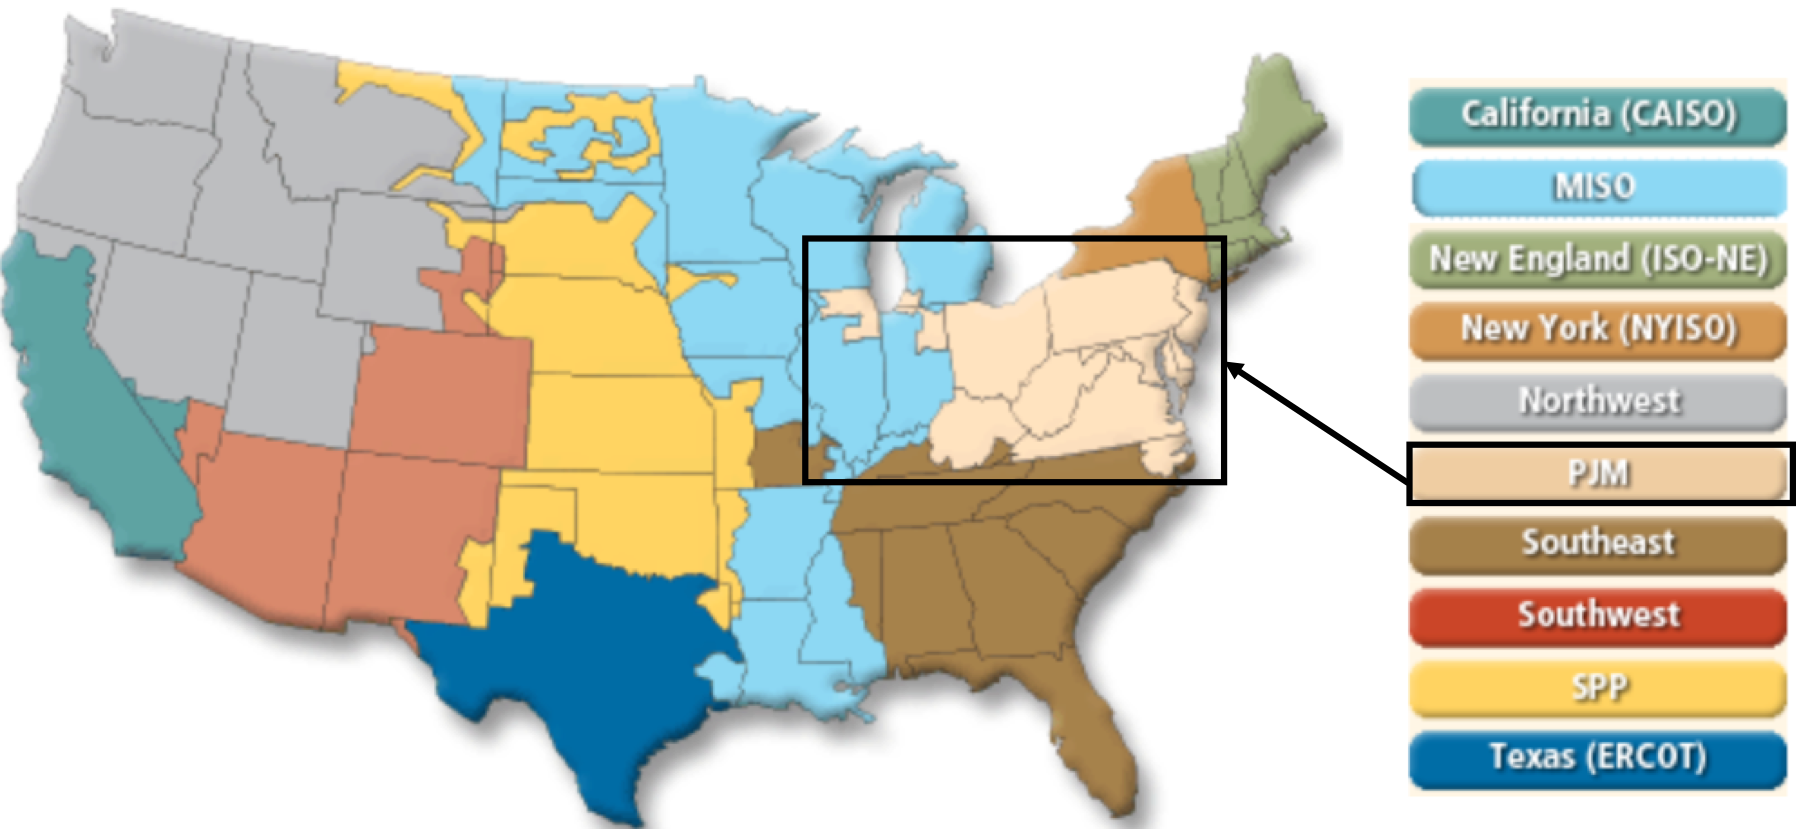
\includegraphics[width=0.95\linewidth]{Figures/US_PowerMarkets}
	\caption{The geographic coverage of electricity markets in the US \cite{FERC_web}}
	\label{fig:pjm-map}
\end{figure}

PJM is regulated by the Federal Energy Regulatory Commission (FERC). Leading utility companies in PJM power markets include Commonwealth Edison, American Electric Power (AEP), Pennsylvania Power \& Light (PP\&L), etc.

\subsubsection{Case 2: DE}

The second case refers to the power market in Germany. The definition is less straightforward compared to the first case, since market organizations are unbundled from the physical systems. 

First of all, we define the physical scope as physical activities of power systems including generation, transmission \& distribution, and consumption in the territories of 4 TSOs, i.e. TenneT, 50Hertz, Amprion and TransnetBW, which operate the power grids covering the whole geography of Germany, illustrated by Figure \ref{fig:germany-map}. 

\begin{figure}[h!]
	\centering
	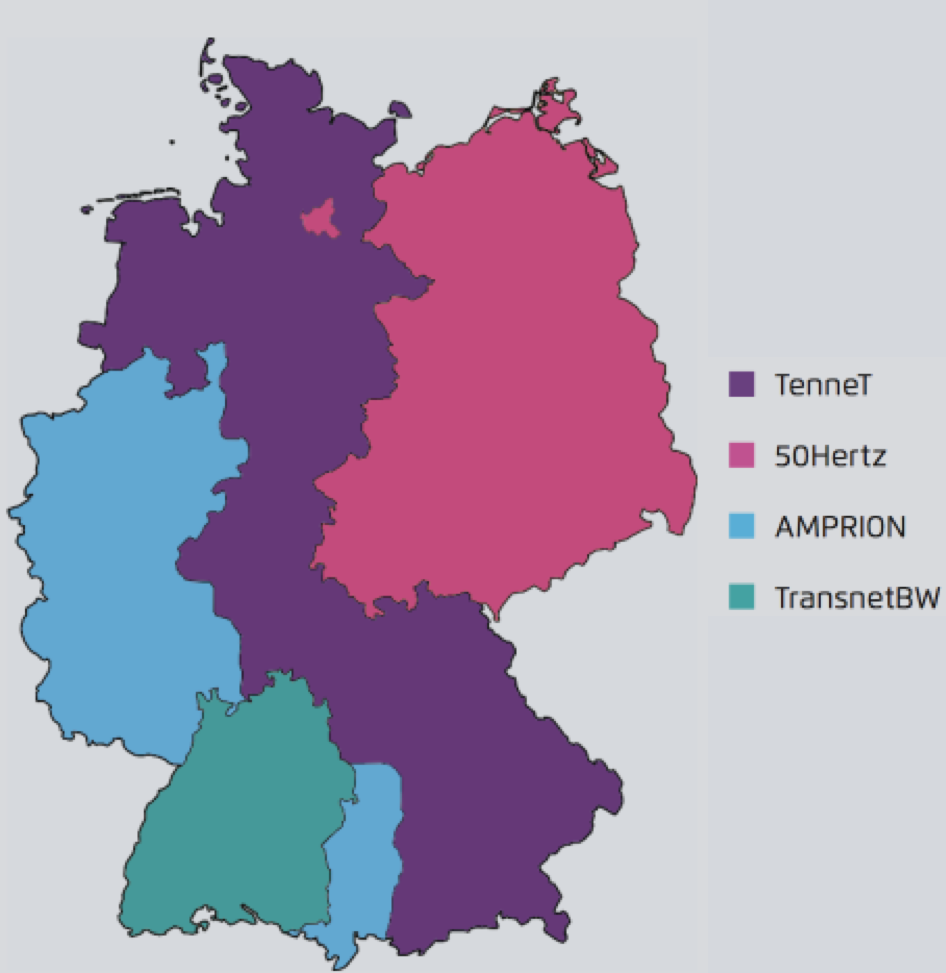
\includegraphics[width=0.7\linewidth]{Figures/Germany_TSOs}
	\caption{The geographic coverage of 4 TSOs in Germany \cite{Bayer2015}}
	\label{fig:germany-map}
\end{figure}

On the market aspect, the electricity market is fully liberalized and transactions can be made either through bilateral agreements over the counter (OTC) or through centralized power exchange. Major power exchanges include the European Energy Exchange (EEX) in Leipzig for forward products and the EPEX SPOT in Paris for spot trading. EPEX SPOT organizes a day-ahead market and an intra-day market. Territories of TSOs in Germany and Austria are coupled in a single bidding zone in the day-ahead market. Increasing proportion of electricity transactions is observed to made through EPEX SPOT \cite{Bayer2015}. In 2016, the trading volume in the Germany/ Austria day-ahead market of EPEX SPOT was equal to over 45\% of the total electricity demands in Germany\footnote{Own calculation based data described in Appendix \ref{sec:accounting-data-prepare}}. 

Ancillary services in Germany are responsible by the 4 TSOs and coordinated by German Grid Control Cooperation (in German Netzregelverbund, NRV). NRV was established by the German TSOs in 2012 and since it was founded, market activities for ancillary services among 4 TSOs have been unified.

There is no capacity market existing in Germany.

The regulator for electricity sector is the Federal Network Agency (in German Bundesnetzagentur, BNetzA) and major utility companies include RWE, E.ON, EnBW, and Vattenfall, often referred to as the ``big 4".

\subsubsection{Case 3: NSW}

Case 3 refers to the pricing zone of New South Wales in Australia's National Electricity Market operated by Australia Energy Market Operator (AEMO) who is both a MO and a SO.

\begin{figure}[h!]
	\centering
	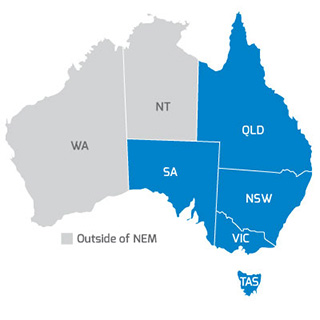
\includegraphics[width=0.7\linewidth]{Figures/AEMO_map.jpg}
	\caption{The geographic coverage and pricing zones of Australia's National Electricity Market \cite{Bayer2015}}
	\label{fig:nsw-map}
\end{figure}

AEMO manages the National Electricity Market (NEM) for the power system in Australia's eastern and south-eastern seaboard, and Wholesale Electricity Market (WEM) for the power system in Western Australia. Within NEM, zonal pricing scheme is applied and market price is settled based on the Regional Reference Price (RRP) for five RRP zone areas: Queensland (QLD), New South Wales (NSW), Victoria (VIC), South Australia (SA) and Tasmania (TAS) \cite{AEMO2010,AEMO_web}, as illustrated by Figure \ref{fig:nsw-map}.

Besides, AEMO operates markets for the delivery of ancillary services in complement to NEM, which are also settled separately in the five RRP zones. 

Among these zones, NSW is selected since it is the largest segment in terms of aggregated trading volume \cite{AEMO_web}, metering points \cite{NortheastGroup2017a} as well as population.

AEMO is governed by the Australian Energy Market Commission (AEMC) that is responsible for developing and making rules, and is regulated by the Australian Energy Regulator (AER) \cite{AEMO_web}. Key utility companies in New South Wales include Origin Energy, Energy Australia and AGL.

\subsubsection{Indication of general market scale}

Table \ref{tab:case-statistics} lists the key statistics that characterize physical properties of three cases. It should be able to provide readers an intuitive comparison of the general scale between different cases. Moreover, some numbers will be used as metrics in quantiative studies to be discussed in Section \ref{sec:quantitative}.

\begin{table}[h!]
	\small
	\centering
	\begin{tabular}{L{0.4\linewidth} R{0.1\linewidth} R{0.1\linewidth} R{0.1\linewidth}}
		\hline
		\textbf{Item} & \textbf{PJM} & \textbf{DE} & \textbf{NSW}\\
		\hline
		Population covered (million) & 65.0 & 82.7 & 7.5\\
		Metering point (million) & 30.3&51.9 &3.4  \\
		Generation capacity (MW, 2016) & \num{176569}& \num{200888}  & \num{16319}  \\
		Consumption (2016) & & & \\
		\multicolumn{1}{r}{\textit{Average rate, in MW}} & \num{87793} & \num{59138}&\num{7978} \\
		\multicolumn{1}{r}{\textit{Aggregated volume, in TWh}} & 771.2& 519.5& 70.1\\
		\hline
	\end{tabular}
\caption{Key statistics for comparison of scale across three cases }\label{tab:case-statistics}
\end{table}

From Table \ref{tab:case-statistics}, we can notice that PJM and DE are roughly on the same scale while NSW is one order of magnitude smaller than the other two.
\section[Qualitative assessment on market regimes and business opportunities]{Qualitative assessment on market regimes and business opportunities%}
	\sectionmark{Qualitative assessment}}
\sectionmark{Qualitative assessment}
\label{sec:qualitative-analysis}

In this section, we first apply the analytical framework established in Chapter \ref{ch:market} to characterize and compare the market regimes in three cases, followed by detailed analysis of each case, based on which we identify potential business opportunities for flexibility solutions in those three regions.

Table \ref{tab:qualitative-comparison} presents a high level comparative description of the market design in three cases.

\begin{table}
	\footnotesize
	\centering
	\begin{tabular}{L{0.25\linewidth} R{0.25\linewidth} R{0.25\linewidth} R{0.25\linewidth}}
		\hline
		\textbf{Characteristic} & \textbf{PJM} & \textbf{DE} & \textbf{NSW}\\
		\hline
		&&&\\
		\multicolumn{4}{l}{\textit{\textbf{Energy market}}} \\
		&&&\\
		Power pool (PP) or power exchange (PX) &  PP& PX & PP\\
		&&&\\
		Demand-side participation & Yes & Yes & In process\\
		&&&\\
		\multirow{3}{*}{Marketplace} & Day-ahead & Day-ahead & \multirow{3}{*}{Real-time}\\
		\multirow{3}{*}{} & & Intra-day & \multirow{3}{*}{}\\
		\multirow{3}{*}{}&Real-time & Balancing & \multirow{3}{*}{} \\
		&&&\\
		Pricing scheme & Nodal pricing & Zonal pricing & Zonal pricing \\
		&&&\\
		\hline
		&&&\\
		\multicolumn{4}{l}{\textit{\textbf{Frequency control ancillary service market}}} \\
		&&&\\
		Marketplace & & &\\
		\multicolumn{1}{r}{\textit{Primary control}} & \textit{No market}  & Primary control\footnote{In this thesis, we will adopt the terminology as: primary control reserve (PCR), secondary control reserve (SCR), and tertiary control reserve (TCR). It shall be noted that in the literature, they are sometimes referred to as frequency containment reserve (FCR), automatic frequency restoration reserve (aFRR), and manual frequency restoration reserve (mFRR), respectively. Alternatively, PRL, SRL and TRL can be used as abbreviations from the German expressions, Prim{\"a}rregelleistung, Sekund{\"a}rregelleistung and Terti{\"a}rregelleistung.} & Contingency Lower (Fast, Slow, Delayed), Contingency Raise (Fast, Slow, Delayed)\\
		\multicolumn{1}{r}{\textit{Secondary control}} & Regulation RegD, Regulation RegA  &  Secondary control$^a$ & Regulation Lower, Regulation Raise\\
		\multicolumn{1}{r}{\textit{Tertiary control}}  & Synchronous, Non-synchronous, Supplementary &  Tertiary control$^a$  &\textit{No market} \\
		&&&\\
		Demand-side participation & Yes & Yes & In process \\
		&&&\\
		Market model & Decentralize & Centralize & Centralized\\
		&&&\\
		\hline
		&&&\\
		\multicolumn{4}{l}{\textit{\textbf{Capacity remuneration mechanism}}} \\
		Capacity market & Yes & Energy-only & Energy-only \\
		Other remuneration mechanism& - & Interruptible loads & Emergency DR\\
		Demand-side participation & Yes & Yes & Piloting \\
		&&&\\
		\hline
	\end{tabular}
	\caption{Comparison of power market regimes in three cases}\label{tab:qualitative-comparison}
\end{table}

It can be seen that market structures are indeed diverse among the three cases, but generally these three regimes hold positive altitude toward emerging flexibility solution.

Overall, PJM offers the most comprehensive routines and most favorable framework for flexibility solutions participating in wholesale markets. Through its specially designed ``Demand Response" program, all kinds of behind-the-meter flexibility solutions can participate in all segments of its power markets, including energy, capacity and ancillary service markets\cite{PJMInterconnection2017}. Furthermore, PJM has implemented a separate frequency regulation marketplaces, named Regulation Dynamic (RegD), exclusive for emerging flexibility resources with fast response. The RegD design offers many merits that are favored by emerging flexibility resources, including higher performance payment and energy-neutral signals. Besides, PJM has nodal pricing scheme using LMP model which is also favorable for small-scale flexibility resources as discussed in Chapter \ref{ch:market}. 

In DE, its fully liberalized electricity market is theoretically non-discriminatory to all technologies and thus there are no explicit hurdles against emerging flexibility solutions. However, there are few incentives either, that encourage the participation of emerging flexibility technologies. Besides, the pre-qualification and product designs of frequency control services are not favored by emerging flexibility sources which implicitly becomes a barrier for their participation.

In NSW, AEMO is proactively innovating its market designs aiming at more incentives for flexibility solutions. In 2013, AEMO has proposed demand response mechanism that offers aggregators the same rights as other retailers or large generators \cite{AEMO_DR_1}. However, many of the implementations are still at pilot stage \cite{AEMO_DR,AEMO_DR_Pilot}.

More details are providing in the remainder of this section.

\subsection{Opportunities of flexibility solutions in PJM}

\subsubsection{Power market structure}

The power market structures and important rules are summarized based on the official manuals published by PJM \cite{PJM2017b,PJM2017c,PJMInterconnection2017,PJM_web}.

PJM is a power market with capacity obligation. Utilities and other electricity suppliers operating in PJM' territory is required to have adequate resources to meet their customers' demand plus a reserve. Such requirements on capacity availability can be met by market participants with their own generating capacity, or with capacity purchased from others under bilateral contracts or with capacity obtained through PJM capacity market auctions. In PJM, curtailable loads are deemed as supply-side resources and are eligible to receive capacity payments.

Besides the capacity market, PJM operates energy and ancillary service markets, as illustrated by Figure \ref{fig:pjm-market-structure}.

\begin{figure}[h!]
	\centering
	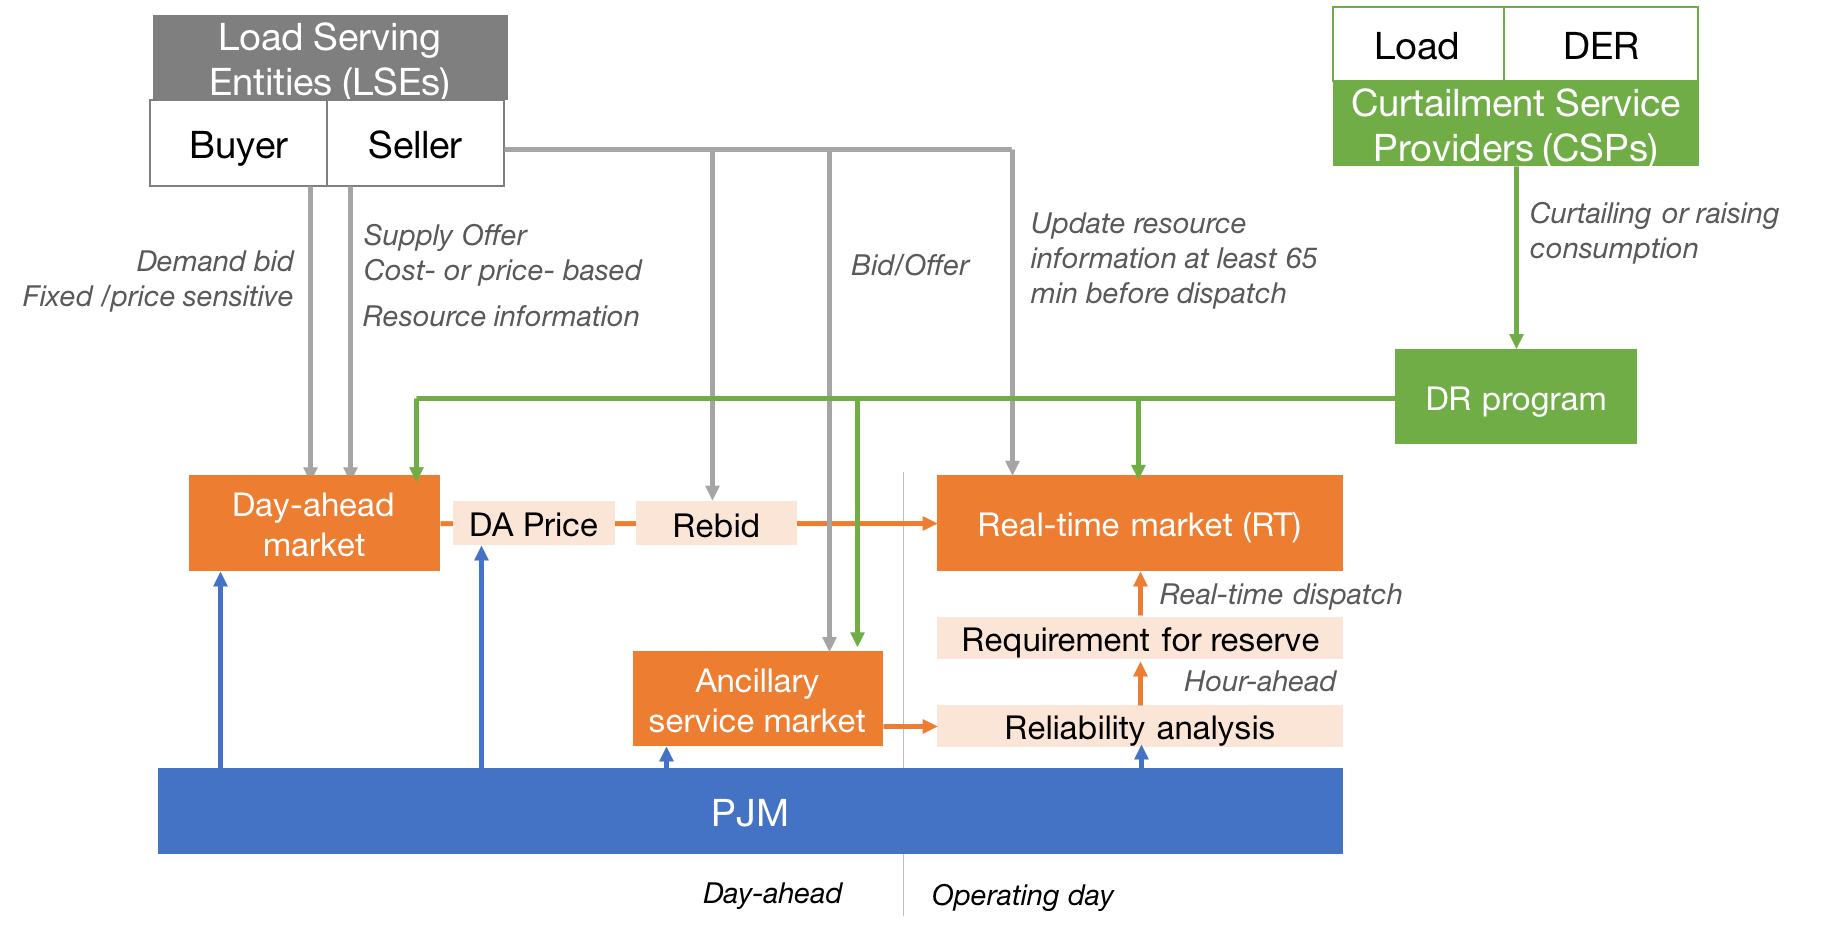
\includegraphics[width=0.95\linewidth]{Figures/PJM_market-structure}
	\caption{Power market structure in PJM}
	\label{fig:pjm-market-structure}
\end{figure}

Being a power pool, all bulk energy transactions have to first go through the day-ahead market, which is organized every day during 8:00-10:30. PJM requires its market participants, named load serving entities (LSEs), to provide information on generation offer, demand bid as well as self-scheduled bilateral transactions, based on which hourly prices are calculated for the next operating day. Generation offers need to be submitted along with physical parameters of the resources, as a common exercise of power pools introduced in Chapter \ref{ch:market}. Demand bids are usually simple indication of quantities but PJM has implemented special measures to enable price-sensitive bids \cite{PJM2015,PJM2017b}. After the day-ahead market closure, generators are able to make rebid and have the obligation to constantly update its resource information till 65 minutes prior to dispatching. PJM constantly monitors the participants' performance. If a participant fails to fulfill its commitment without informing PJM in advance, its participation might be suspended until certain measures are taken. All energy transactions occur after day-ahead market closure will be settled in the real-time market. Real-time market calculates prices in five-minute intervals, but transactions are settled hourly.

In terms of ancillary service market, PJM operates four markets for ancillary services, i.e. regulation, synchronous reserve, non-synchronous reserve and supplementary reserve. Regulation is close to the concept of secondary control reserve, while the others are similar to tertiary control reserves, in the UCTE standard, as introduced in Section \ref{sec:market-as}. Minimum scale of resource to provide ancillary services is 0.1 MW so favors small-scale flexibility solutions. 

Regulation products are not separated to up/ down regulation, but there are two products, named regulation dynamic (RegD), and regulation conventional (RegA). RegD is designed specifically for emerging solutions. It was first developed in 2012, following the Order 755 of FREC which called for more equitable treatment for fast responding resources
\cite{FERC755}. RegD offers higher performance payment to reward the fast responding nature of new technologies and the signal is engineered to be conditional neutral within 30 minutes\footnote{The signal was originally neutral within 15 minute but in January 2017, it was re-engineered \cite{PJM2017b}.}. However, since imbalance in grid is usually not energy-neutral, a energy-neutral signal cannot fully fulfill the needs of regulation by its own so in PJM the RegD is constrained to be no more than 26.2\% of total regulation capacity. 

Ancillary services are paid for the capacity provided as well as the actual performance using a special algorithm calculating a performance score (referring to Appendix \ref{sec:accounting-data-prepare}). Capacity bids and offers are submitted in hourly block to PJM through market gateway between 13:30-14:30 day-ahead. The hourly time-slice of product offers great operational flexibility of resources. In the operating day, PJM will continuously run its reliability analysis and determine the amount of capacity required for next operating hour as well as determine the market clearing price. All the energy delivery dispatched in the real-time is settled in the real-time energy market. Therefore, we can see the real-time energy is the hub for all real-time operations.

\subsubsection{Storage, aggregator and demand-side participation}
PJM allows demand-side resources to participate in all of its market segments, including capacity, energy and ancillary services, through the so-call ``demand response (DR) program"  \cite{PJMInterconnection2017}. The entities that provide demand response services are named curtailment service providers (CSPs), which can be LSEs or third-party companies. CSPs are allowed to aggregate loads and operate them as flexibility sources by either shifting or curtailing certain amount of loads. Since PJM do not regulate the behind-the-meter behaviors, the DR program is actually a gateway for all behind-the-meter distributed energy resources (DERs). However, it should be noted that CSPs are not allowed to inject energy beyond the meter to the grid, which limits some energy-intensive DERs whose outputs cannot be fully digested by local demands. PJM stated notice on this issue and claim it is currently under discussion in Special Market Implementation Committee meetings \cite{PJMInterconnection2017}.

Besides the behind-the-meter DERs, grid-scale energy storage systems are allowed to participate in the ancillary service markets and are actually the primary target resources of the RegD product with an energy-neutral signal. However, the participation of storage assets in energy markets (excluding pumped hydro storage) is still uncertain. In March 2018, FERC issued a new order to urge the ISOs to implement market gateways for storage systems in their energy markets \cite{FERC841}. The effectiveness of the order is still remaining to be seen.

%PJM DR is the umbrella for all distributed energy resources, including DR, behind-the-meter generations, storage, etc. since PJM does not specify how the load is reduced. However, PJM DR program does not allow energy injection beyond the meter and receive wholesale compensation.\cite{PJMInterconnection2017}. This issue is currently under discussion in Special Market Implementation Committee meetings.

%DR emergency fast changing over years \cite{Brown2015}
%Since the DR in the wholesale market as a supply recouse will cause double payment issue where a customer may receive wholesale energy revenue and retail cost savings for the same MW of load reduction, PJM states that DR participation in the retail market on the demand side would be more ideal. And they are discussing to revisit the mechanism. Therefore, this value is not fully modeled in our study.

\subsubsection{Summary and analysis of business opportunities}
In PJM, all behind-the-meter distributed energy resources, such as distributed generation, load-shifting applications, and energy storage systems, are allowed to participated in all of its marketplaces by altering the load profile (but not allowed to inject energy beyond the meter). Grid-scale BESS is allowed to participate in ancillary service market but is not waiting for implementation to direct play in energy market. 

Therefore, all three applications we proposed at Chapter \ref{ch:introduction}, i.e. arbitrage in energy market, frequency control in ancillary service market, and supply adequacy in capacity market,  are feasible using all kinds of technologies. Moreover, the additional incentives such as the specially designed RegD product exclusively for emerging flexibility solutions makes PJM the best example that embraces new technologies for flexibility provision.

\subsection{Opportunities of flexibility solutions in DE}
\label{sec:quali-de}
\subsubsection{Power market structure}

Information and rules about the power markets in Germany are mainly sourced from the official websites of the TSOs \cite{Hertz_web,Amprion_web,TenneT_web,TransnetBW_web,DE_as_web} as well as from other literature \cite{Moller2010,ConsentecGmbH2014,Wartsila2014}.

The power market structure in Germany is illustrated by \ref{fig:de-market-structure}.

\begin{figure}[h!]
	\centering
	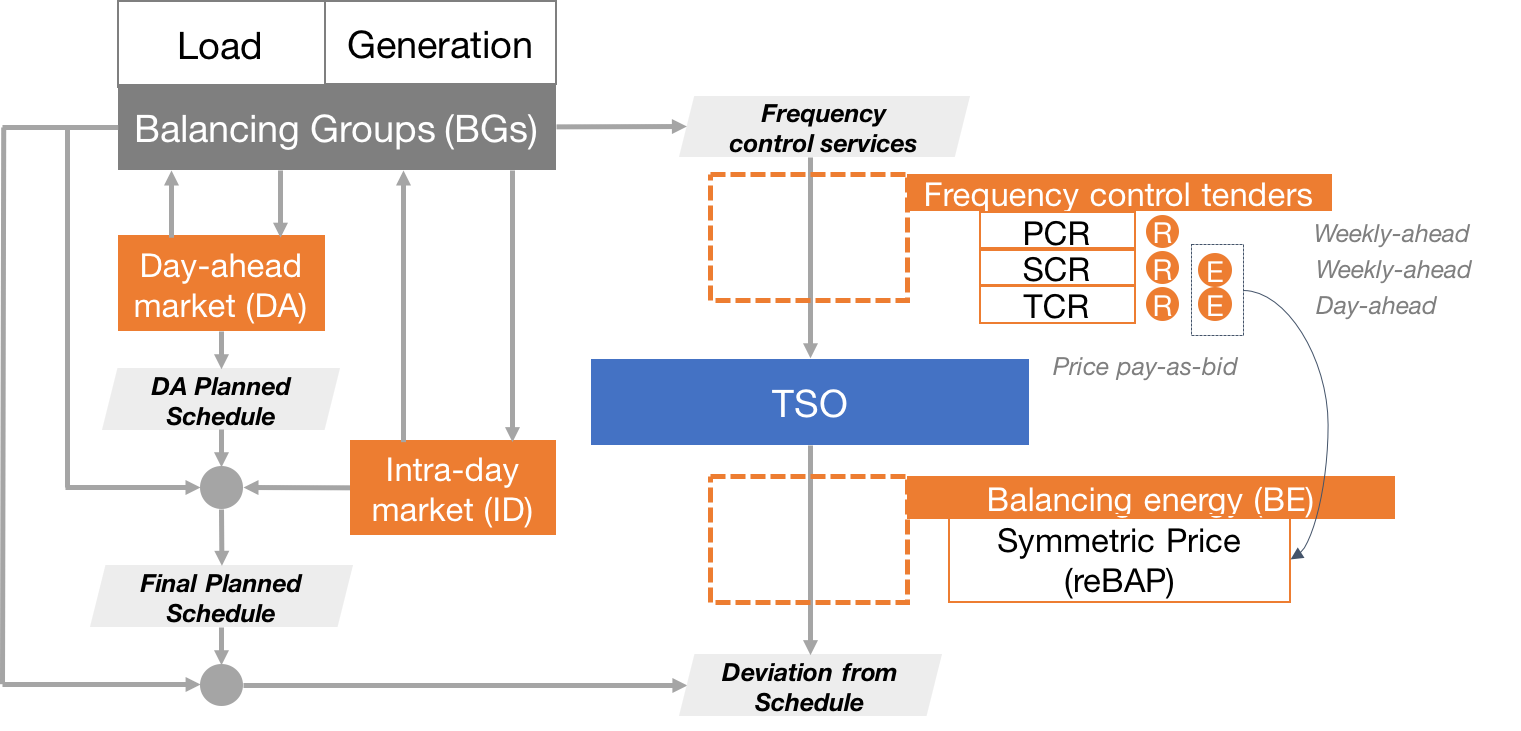
\includegraphics[width=0.95\linewidth]{Figures/DE_market-structure}
	\caption{Power market structure in Germany}
	\label{fig:de-market-structure}
\end{figure}

In Germany, market participants are organized into balancing groups (BGs, in German Bilanzkreise). 
BGs can be made up with large generators, or aggregations of smaller generators, or aggregated loads, or the mix of them. Therefore, such a model naturally fits the concept of aggregators. BGs are organized and regulated in standard balancing group contracts provided by TSOs.

BG operators is responsible for following the planned schedules which derived from their positions in energy markets, including day-ahead, intra-day and bilateral contracts. In real-time actual physical flow are monitored in every 15 minutes. Any deviations from the planned schedule lead to financial settlement through the balancing energy pricing scheme that is unified over the whole of Germany, known as ``reBAP" abbreviated for the German expression ``regelzonenuebergreifender einheitlicher Bilanzausgleichsenergiepreis". The reBAP is a symmetric price, i.e. imbalance volumes in both direction are settled with a single price. The reBAP is calculated in every 15 minutes as:

\begin{equation*}
\text{reBAP} = \frac{\sum \left( \text{balancing energy costs - balancing energy revenues}\right)(\text{EUR})}{\text{net imbalance volume} (\text{MW})}
\end{equation*}
where, the balancing energy costs and revenues are the payments occur by activating secondary and tertiary frequency control reserves, and the net imbalance volume is the single aggregation of volumes in every 15-minute interval. It can be conceived that net imbalance volume could be close to zero sometimes which leads to extreme high reBAP. Therefore, to avoid such situations, reBAP is capped at the marginal price of balancing energy used in that period. However, such a price formation mechanism still results in high price volatility.

Since the charge from reBAP could be considerably high, BGs may seek solutions to balance deviations by themselves. In those cases, deploying flexibility resources could be an option for them.
 
Besides, prior to the calculation of reBAP, TSOs allows post-scheduling trading between BGs for them to net their imbalance positions. However, there is no organized markets for these activities so BGs have to find the counter-parties by themselves or through brokers. 

On the system level, the overall imbalances that are not offset between BGs have to be tackled by TSOs by activating frequency control services. In Germany, the centralized model as introduced in Section \ref{sec:market-as}, is applied. 4 German TSOs organizes joint tenders for procurement of these services. Prices for services are determined using the pay-as-bid scheme. For secondary and tertiary control reserve (SCR and TCR), capacity and energy is priced separately while for primary control (PCR) only capacity is priced. Costs incurred for activating SCR and TCR energy is recovered through reBAP as discussed earlier, while costs for procuring capacity are socialized among all market participants, being collected in network charges. More details regarding tenders for purchasing frequency control services are listed in Table \ref{tab:de-tender}.

\begin{table}[h!]
	\footnotesize
	\centering
	\begin{tabular}{L{2.5cm} L{2.5cm} L{2.5cm} L{2.5cm}}
		\hline
		& \multicolumn{1}{l}{\textbf{PCR}}& \multicolumn{1}{l}{\textbf{SCR}}& \multicolumn{1}{l}{\textbf{TCR}} \\
		\hline		
		&&&\\
		Tender period & weekly & weekly & daily\\
		&&&\\
		product time-slice & none (whole week) &  peak/ off-peak\footnote{Peak block covers 8am-8pm for Monday to Friday, while the residual of period belongs to off-peak block.} & 6 hours (4 blocks per day) \\
		&&&\\
		minimum bid & 1 MW & 5 MW & 5 MW\\
		&&&\\
		call for tender & capacity price merit-order & energy price merit-order & energy price merit-order\\
		&&&\\
		remuneration & pay-as-bid (capacity only) & pay-as-bid (capacity and energy) & pay-as-bid (capacity and energy)\\
		&&&\\
		\hline
	\end{tabular}
	\caption{Characteristics of frequency control reserve products tendered in Germany\cite{DE_as_web}}\label{tab:de-tender}
\end{table}
~\newpage
\subsubsection{Storage, aggregator and demand-side participation}
Theoretically, with the market organized in balancing groups, aggregators of emerging flexibility resources can also form their own BGs and participate in all market segments. However, without special incentives, new players may face adverse positions in computing with well-established BGs which is typically large in scale. Besides, in the frequency control market, although there are no explicit rules against emerging flexibility technologies, the current pre-qualification rules are not favorable for emerging technologies. 
According to the data published by TSOs \cite{DE_as_web}, emerging flexibility solutions account only for a niche proportion of pre-qualified frequency control resources, as shown by Table \ref{tab:as-flexibility-share}.

\begin{table}[h!]
	\small
	\centering
	\begin{tabular}{l r r r r r}
		\hline
		\textbf{Technology} & \textbf{PCR} & \textbf{SCR+} & \textbf{SCR-} & \textbf{TCR+} & \textbf{TCR-} \\
		\hline
		BESS & 0.18 & - & - & -&-\\
		\multicolumn{1}{r}{\textit{share (\%)}} & \textit{3.3} & - & - & - & - \\
		DR & 0.07 & 0.51 & 0.61 & 0.78 & 0.69 \\
		\multicolumn{1}{r}{\textit{share (\%)}} & \textit{1.3} & \textit{2.3} & \textit{2.7} & \textit{1.9} & \textit{1.7} \\
		\hline
		Total (in GW) & 5.44 & 22.42 & 22.50&40.56& 39.7\\
		\hline
	\end{tabular}
\caption{Overview on pre-qualified capacity (in GW) for frequency control service in Germany}\label{tab:as-flexibility-share}
\end{table}

Besides, some product designs also implicitly create barriers for some flexibility solutions, such as:
\begin{itemize}
	\item Non-energy-neutral signals: as discussed previously, energy-neutral signals fit the technical requirements of flexibility solutions that do not generate energy. However, energy-neutral signals are not an implementation in Germany.
	\item Large product time-slice: all services have to offer in large blocks as shown by Table \ref{tab:de-tender}, which requires the resources to sustain the committed available over a long period of time. This reduces the operational flexibility for resource owners significant. Especially for some flexibility solutions 
\end{itemize}

\subsubsection{Summary and analysis of business opportunities}

Overall, since the power market in Germany is fully liberalized with the physical system operation and market activities unbundled, there are no explicit barriers for emerging technologies in the market. Flexibility solutions can participate in any of the marketplaces. However, due to the lack of incentives and existence of implicit hurdles as discussed previously, new players with a portfolio of purely emerging flexibility solutions may face an adverse situation while competing with other existing players.

A more pragmatic approach, rather than operating the emerging flexibility solutions alone, could be operating them as a part of the portfolio of existing BGs and complement other resources participating in the market to avoid imbalance charges as mentioned previously. Nevertheless, such an arrangement should not be favorable for technology vendors of flexibility solutions, since the customers would be in a stronger position. Moreover, since the new flexibility solutions are in fact competing with existing portfolio, the established players with large portfolio of conventional assets may lack motivations to embrace new technologies.

\subsection{Opportunities of flexibility solutions in NSW}

\subsubsection{Power market structure}

The power market in NSW is part of the Australia's NEM operated by AEMO. Therefore, while analyzing the power market structures, we refer the power market in NSW to NEM. Analysis on are mainly based on the actual market rule \cite{AEMC_rule} and the documents published by AEMO \cite{AEMO2010,AEMO2013,AEMO2015,AEMO_DR_1,AEMO_web} as well as other literature \cite{Wang2015,Brown2015,Srivastava2011,NortheastGroup2017a}.

The structure of NEM is illustrated by \ref{fig:nsw-market-structure}.

\begin{figure}[h!]
	\centering
	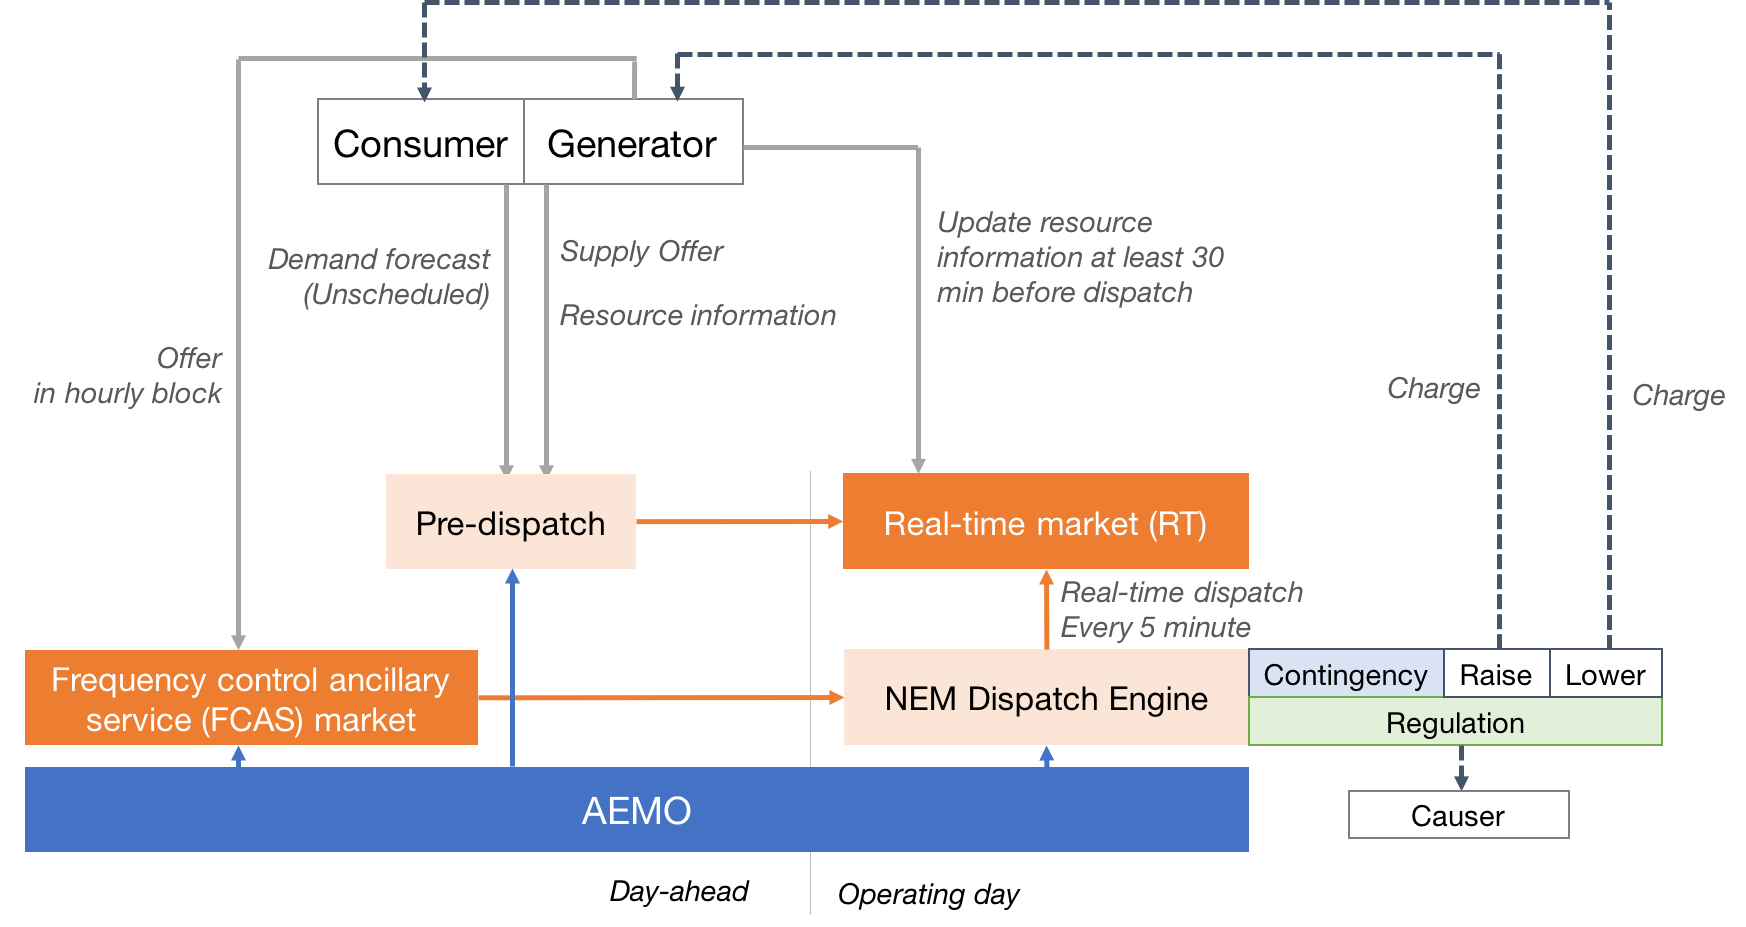
\includegraphics[width=0.95\linewidth]{Figures/NSW_market-structure}
	\caption{Power market structure in NSW (NEM)}
	\label{fig:nsw-market-structure}
\end{figure}

The NEM is generally similar to PJM as both are organized in the power pool model. Participation is mainly from the generation-side, while demands are largely remain unscheduled. Offers and information submitted to AEMO in the day ahead are only for scheduling and pre-dispatch. All the transactions are settled in the real-time market. Currently, the real-time market is with a 5-minute dispatching and pricing interval, while the settlement interval is half-hour. 

Ancillary services in NEM are categorized into three groups: Frequency Control Ancillary Services (FCAS), Network Support \& Control Ancillary Services (NSCAS), and System Restart Ancillary Services (SRAS). Among them FCAS are of our most interest. There are two types and a total of eight products in FCAS markets, namely:
\begin{itemize}
	\item \textbf{Regulation}: used to correct for minor changes in the demand/ supply balance, and activated by AGC. Therefore, it is close to the concept of secondary control reserve in UCTE standard. Regulation products are separated to Raise/ Lower:
	\begin{itemize}
		\item Regulation Raise: used to correct a minor drop in frequency;
		\item Regulation Lower: used to correct a minor rise in frequency.
	\end{itemize}
	\item \textbf{Contingency}: used to correct for major changes in the demand/ supply balance, and activated by local automatic response to frequency. In terms of the activation mechanism, contingency services are close to primary control reserve in UCTE standard. However, the requirements for activation time are distinct. In NEM, slow and delay response are allowed:
	\begin{itemize}
		\item Fast Raise: 6-second response;
		\item Fast Lower: 6-second response;
		\item Slow Raise: 60-second response;
		\item Slow Lower: 60-second response;
		\item Delayed Raise: 5-minute response;
		\item Delayed Lower: 5-minute response.
	\end{itemize}
\end{itemize}

The payment and cost allocation is in the centralized model. AEMO make payment to FCAS providers based on the capacity enabled by NEM dispatch engine (NEMDE) and the market clearing price. On the other hand, AEMO will recover the costs from either the causer (for regulation services) or from the market participants (for contingency services).The amount of recovery charge for contingency services is purely based on their electricity flow as a ratio to the system total flow. Therefore, unlike the DE case, market participants do not have the motivation to market self-balancing.

\subsubsection{Storage, aggregator and demand-side participation}

As mentioned previously, AEMO proposed a demand response mechanism (DRM) in 2013 \cite{AEMO_DR_1}. In this designed scheme, AEMO planned to enable the DR aggregators to register as the same as retailers or generators in particular Demand Response Intervals. AEMO proposed an algorithm that forecast a baseline load for each Demand Response Interval  based on historical data with and without DR. Such a baseline will be compared with actual consumption to determine the payments fro DR aggregators. Therefore, in order to implement such an algorithm, pilot projects \cite{AEMO_DR_Pilot} as well as more information regarding demand-side participation \cite{AEMO_DR} are required. For these reasons, the DRM is not yet fully rolled out for the whole NEM.

Regarding grid-scale storage, they are currently regulated under interim arrangements \cite{AEMO_BESS}, where storage units are allowed to participate in both energy and FCAS markets. In energy market, a storage unit has to register as both a generator and consumer. 

\subsubsection{Summary and analysis of business opportunities}

As we have seen, market for flexibility solutions in NSW is at a transition state. AEMO is proactively pursuing more incentives for emerging technologies although most of the implementations are not complete. However, it is anticipated that the current barriers for new technologies will gradually be removed by the on-going re-structures.

So far, participation of aggregators and demand-side resources are still limited, but grid-scale storage assets are able to participate in all market segments.


\subsection{Summary and implications}

Based on the qualitative analysis provided above, we have seen that situations vary significantly among the cases. In markets organized in power pool model, the bundled physical and market operations have many legacy designs against emerging flexibility solutions. PJM has made successful actions to remove most of these barriers to grant new technologies more accessibility to its markets. What is remaining to settle, as we have identified, is the direct participation of storage systems in energy markets and the energy injection from behind-the-meter DERs. However, these issues have been noticed by PJM as well as the regulator FERC, and are expected to be resolve in near future. In NSW, AEMO is also proactively seeking to make the same exercise, and the market is at a transition with those on-going restructurings.

However, we have also noticed that even in a fully liberalized power markets like Germany without any explicit barriers, the participation of new technologies are still limited. This implies there might be some implicit barriers caused by market design, e.g. the frequency control product design as mentioned previously. Alternatively, it could be probably because the market size and profitability of emerging technologies are not attractive enough to investor, or at least were not attractive. With fast development of technologies, costs of some technologies are dropping rapidly. Besides, market conditions have been also evolving with increasing penetration of RES generation. A renewal of the views would be necessary. 

Understanding possible impact of implicit barriers and updating the view on market size and profitability with fast changing conditions are both tasks that need to be settled by quantitative works. In order to achieve these goals, we would assume those explicit barriers have been removed so that we can focus on a deeper layer beyond that, while impacts of these explicit barriers have generally been analyzed in this section using qualitative approach.



%\subsubsection{Players}
%A Load Serving Entity (LSE), as is defined officially by PJM, is "any entity that has been granted authority or has an obligation pursuant to state or local law, regulation, or franchise to sell electric energy to end-users that are located within the PJM RTO. An LSE may be a Market Buyer or a Market Seller"\cite{PJM2017b}. Therefore, LSEs refer to all market participates in PJM who have rights and obiligation to act in all the power marketplaces of PJM, including the energy, capacity and ancillary services markets. 

%Curtailment Service Providers (CSPs) are members in PJM markets specializing in demand response. A CSP is an intermitted agency that provides the end-user DR to the wholesale market. \cite{PJM2017b} \cite{Wang2015} The role of the CSP is actually a legacy product from the liberalization of retail markets in PJM. Once the retail competition began, PJM allowed LSEs to provide DR not only for their own customer but also for customers of other LSEs. The role of the CSP was created to facilitate the liberalization and competition. \cite{PJMInterconnection2017}

%\subsubsection{Balancing mechanism}
%submit offer - rebid - update information up to 65 mins - deviation charged with real-time

%reviewed the participation, violating -> suspend activity, enter enforcement

%LSE obiligate to purchase (or self-schedule) reserve, obiligation as a proportion to its contributing flow to the grid. \cite{PJM2017c} This incents liquidity in the market with competitions on both buyer's and seller's side. However, the obiligation does not reflect their actual needs.\cite{Wartsila2014}

%CSP
%ntermitted agency
%allowed to voluntarily respond to the LMP

%\subsubsection{PJM DR}

\section[Quantitative studies and results on market size and profitability]{Quantitative studies and results on market size and profitability%}
	\sectionmark{Quantitative results}}
\sectionmark{Quantitative results}
\label{sec:quantitative}
%So far we have elaborated qualitatively the potential opportunities for flexibility solutions in the three geographies.  it is necessary to perform quantitative analysis in order to understand:
As discussed, the primary goal of quantitative studies to understand the:

\begin{itemize}
	\item \textbf{Market size:} the potential value creation in the market for flexibility solutions, subject to certain generic system dynamics but without respect to cost dynamics of specific technologies; and
	\item \textbf{Profitability:} the metric to judge whether a specific technology is profitable or not to extract certain amount of value from current or future markets taking into account cost elements.
\end{itemize}

Based on these results, further analysis on implicit barriers due to unfavorable market designs that are not fully demonstrated by qualitative analysis, can performed.

For estimation of the maximum market potential for flexibility solutions in general, a energy storage system is adopted to as a generic representative technology. Energy storage is selected because it has fewer dependencies on external factors and can be purely utilized for flexibility provision. 
%Unlike many other flexibility solutions, energy storage systems have fewer dependencies on external factors but can be purely utilized for flexibility solution. 
A counter example could be the demand response using air conditioning, the users' comfort need to be considered which creates more constraints in operating the flexibility resources. We further discard all costs associated but only research the value of revenues. Thereby, while the system is made to have ``ample size", derived results shall be able to indicate a maximum market potential. We will define certain scenarios where the system is conceived to have ``ample size".

However, such a market potential might not be really achieved, when costs are taken into account. In addition, for other type of flexibility solutions such as demand responses, as mentioned above, there are more constraints that limit the system to capture the full potential value from markets. Therefore, it is necessary to further understand the market potential and profitability of some specific technologies considering cost dynamics. For this sake, we performed experiments with battery energy storage system (BESS) and electricity vehicle to grid (EV2G) systems, as introduced in  Chapter \ref{ch:methodology}. BESS is taken as a typical energy storage technology and EV2G is considered as a specific type of demand responses. 

As discussed in both Chapter \ref{ch:LitRev} and Chapter \ref{ch:methodology}, we include two types of works in the quantitative part, i.e. using historical power market data and using simulated data considering changed market conditions. The former approach allow us to establish a comprehensive understanding toward the value of flexibility management in nowadays' power markets, while the latter may provide us valuable guidance on the directional movement of the market and thus offer viable references for technology vendors' decision makers.

\subsection{Setup of quantitative cases}
\label{sec:quant-case-setup}
\subsubsection{Data and parameters}
\label{sec:data-parameter}

In order to obtain the expected results as discussed above, we need to find reliable data and parameters for further studies. The details about the sources and preparation of data, as well as the determination of parameters can be found in Appendix \ref{Appendix-data}. Hereby, we provide a high-level overview of them.

\begin{itemize}
	\item Data and parameters for market-based modules, for each market regime including:
	\begin{itemize}
		\item Existing marketplaces, i.e. the elements to make up the sets $\mathbb{I}$ and $\mathbb{I}$;
		\item Price signals, including prices for energy and capacity in all marketplaces;
		\item Liquidity constraints, i.e. trading volumes in all marketplaces;
		\item Frequency control signals;
		\item Generation data by fuel type.
	\end{itemize}
	\item Data and parameters for technology-based modules, for each technology type including:
	\begin{itemize}
		\item System parameters, e.g. efficiencies, energy-to-power ratio (the ratio of nominal energy capacity to power rate), etc.;
		\item Cost parameters, i.e. the parameters required as inputs for the cost module, referring to Section \ref{sec:cost};
		\item EV model, i.e. battery capacity and (dis)charge rate per EV;
		\item EV driving profiles, which is obtained via simulations based on real-world transportation;
		\item Number of EVs, real-world data for scenario generation.
	\end{itemize}
\end{itemize}

Particularly, it is worth to mention two assumptions that are made for electricity market data in the DE case and may have notable impacts on final results:

\begin{enumerate}
	\item We use the total consumption in Germany as the day-ahead market volume rather the actual trading volumes in EPEX SPOT day-ahead market, for two reasons:
	\begin{itemize}
		\item First, the EPEX SPOT day-ahead market couples the areas of both German and Austrian TSO zones, rather than for Germany only.
		\item For the other two regimes, PJM and NSW, power markets are organized in power pool arrangements so the day-ahead volumes represent the day-ahead forecast for total consumption. In contrast, for Germany, the market ir organized in power exchange model so only a portion of the total transactions are done through EPEX SPOT. 
	\end{itemize}
	Therefore, due to these two reasons, using the consumption data shall be a better option than using the actual day-ahead volume in EPEX SPOT.
	\item The frequency control signals in the DE case are calculated as the ratio between total procured capacity and total actual delivered energy, due to the limited data availability (for PJM where the data is available, we use the actual control signals).An issue associated with this consumption that should be noted, is that for primary control reserve (PCR), the energy delivery is not monitored and accounted for payment. Therefore, our derived control signal for PCR is actually a zero-signal. This does not affect the accounting results but has an impact on technological aspect, which should be noticed as well.
\end{enumerate}

Besides, as mentioned in Chapter \ref{ch:methodology}, we align all the currencies used in different markets to the single currency as USD. The currency exchange rates used to align the currencies used in different markets are determined as the real market data as of January 1st 2018, when 1 EUR is equal to 1.20 USD and 1 AUD is equal to 0.78 USD\cite{Bloomberg}.

\subsubsection{Use cases}

As determined in the scope, we will apply quantitative model for applications including arbitrage in energy market and providing frequency control in ancillary service market. Since there are different marketplaces existing in different regimes, it is worth to first list the business cases covered in each of the market, as shown by Table \ref{tab:biz-cases}. It shall be notice that sometimes we will stack use-cases to perform multitasking.

\begin{table}[h!]
	\small
	\centering
	\begin{tabular}{l l l}
		\hline
		\textbf{Application}  & \textbf{Marketplace} & \textbf{Abbreviation}\\
		\hline
		\multicolumn{3}{c}{\textit{\textbf{PJM}}}\\
		Arbitrage & Day-ahead & DA \\
		Arbitrage & Real-time & RT \\
		Frequency control & Regulation Dynamic & RegD \\
		Frequency control & Regulation Conventional & RegA \\
		&&\\
		\multicolumn{3}{c}{\textit{\textbf{DE}}}\\
		Arbitrage & Day-ahead & DA \\
		Arbitrage & Intra-day & ID \\
		Arbitrage & Balancing energy & BE \\
		Frequency control & Primary control reserve & PCR \\
		Frequency control & Secondary control reserve & SCR \\
		&&\\
		\multicolumn{3}{c}{\textit{\textbf{NSW}}}\\
		Arbitrage & Real-time & RT \\
		Frequency control & Frequency control ancillary services & FCAS\footnote{Due to data availability, only total system size will be referred to while detailed technical analysis cannot be performed.} \\
		\hline
	\end{tabular}
\caption{Business cases studied in quantitative analysis in different regimes}\label{tab:biz-cases}
\end{table}

It should be noted that the use-case of arbitrage in German balancing energy market is a unique one. 
%It can be noticed that there is a unique case where we name the application as self-balancing.
It corresponds to the situation where BGs in DE power markets may turn to flexibility resources to settle their imbalances in avoidance of charged from TSOs using balancing energy pricing scheme reBAP, as discussed in Section \ref{sec:quali-de}. 
Therefore, the players act passively in this market rather than proactively compared to other markets.
This specialty is due to the balancing energy arrangement in Germany is purely for imbalance cost recovery without a gateway for trading activities, while in the other two regimes, real-time markets are available for trading.% In addition, cost recovery for imbalance settlements are made in different way and are not associated with the real-time markets as explained in Section \ref{sec:qualitative-analysis}. Therefore, we decide to introduce a unique term to distinguishing such a use-case in Germany only.
As a result, this case has a special dynamic which would be revealed in the results.

Besides, for frequency control services, we evaluate only the primary and secondary control.

\subsubsection{Scenarios for market potential for flexibility solutions in general}

For estimation of market potential for flexibility solutions in general, we apply a series of scenarios ($si \in \{1,2,\dots\}$) by adding incremental system size until the system is deemed with \textbf{``ample size"}:
\begin{itemize}
	\item The state \textbf{``ample size"} is determined while marginal revenue ($R$, in USD) to system size ($\overline{s}$, in MWh) is diminishing to a very low level. In this study, we take a threshold of 1\%, i.e. the state is research when :
	\begin{equation*}
	\frac{R_{si}-R_{si-1}}{\overline{s}_{si}-\overline{s}_{si-1}} < 0.01
	\end{equation*}
\end{itemize}
Since the marginal revenue is monotonically decreasing in our study due to liquidity constraints, further residual revenue beyond this state should be limited. We ignore the residual value in order to terminate the simulation within reasonable steps.

\subsubsection{Scenarios for profitability and market potential for battery energy storage system}
For studies on battery energy storage systems , we use the same technique:

\begin{itemize}
	\item \textbf{Profitability} is calculated at the scenarios with system in \textbf{``small size"}, referring to situations where the operation of flexibility resources will not be limited by liquidity constraints.
	\item \textbf{Market potential} is determined at the state with \textbf{``profitable size"}. It is determined when the system size is maximized when net profits $P^{\text{net}}$ is positive:
	\begin{equation*}
	\underset{si}{\text{max}}~\overline{s}
	\end{equation*}
	subject to:
	\begin{equation*}
		P^{\text{net}}_{si} \geq 0
	\end{equation*}
	\begin{equation*}
		\overline{s} \in  \{ \overline{s}_{si}\}
	\end{equation*}
	\begin{equation*}
	si \in \{1,2,\dots\}
	\end{equation*}
\end{itemize}

\subsubsection{Scenarios for profitability and market potential for battery energy storage system}
Electric vehicles are not exclusively for providing flexibility to power systems. In fact, the number of EVs can be viewed as purely determined by external factors. Therefore, unlike energy storage systems, we do not assign arbitrary values to the system size and find the scenario based on the profitability analysis. Instead, we take the numbers introduced in Appendix \ref{app:tech} to generate the following scenarios:

\begin{itemize}
	\item \textbf{EV number 2016:} assuming all EVs available by 2016 are contracted for delivering EV2G services
	\item \textbf{EV number 2017:} similar to the first scenario but using the data of 2017
	\item \textbf{2\% market share:} assuming EVs will account for 2\% of the total vehicle number
\end{itemize}

It shall be noted again that the EV number determined for three regions are actually based on the official data in Germany only while the other two regions are projected by assuming same EV number per household, due to limited data availability; referring to Appendix \ref{app:tech} for more details. The number of EV in each region and in each scenario are listed as Table \ref{tab:ev-scenario}.

\begin{table}[h!]
	\small
	\centering
	\begin{tabular}{L{3cm} R{1.5cm} R{1.5cm} R{1.5cm} R{2.5cm}}
		\hline
		\textbf{Scenario} & \textbf{PJM} & \textbf{DE} & \textbf{NSW} & \textit{per household}  \\
		%\hline
		\hline
		EV number 2016 &  \num{74754} &  \num{43713}&  \num{4849}& \textit{0.014} \\
		EV number 2017 &  \num{129246} &  \num{75578}&  \num{8383}& \textit{0.025} \\
		2\% market share &  \num{900000}&  \num{526290}&  \num{58377} & \textit{0.174} \\
		\hline
	\end{tabular}
\caption{The number of EV in each scenario for each case study}\label{tab:ev-scenario}
\end{table}

\subsubsection{Normalization of results}

The direct outputs of our model are annualized values so are in the unit of USD/yr. In order to make the result comparable among different cases, we normalize them with respected to certain bases.

For the market potential, we normalize the result to the aggregated annual consumption (in MWh/yr) that can be found in Table \ref{tab:case-statistics}. Thereby, the normalized results will be in the unit of USD/MWh. The aggregated annual consumption is taken as an indicator of the overall scale of the power system. Besides, in this way, results in USD/MWh can present an intuitive view on how much value is associated with each MWh of electricity consumed. 

In terms of profitability, apart from the profitability ratio, the absolute values such as net profits will be normalized in accordance to the system size, i.e. kWh for ESS and number of EV for EV2G. Thereby, the final results will in the unit of USD/(yr$\cdot$kWh ESS) or USD/(yr$\cdot$EV) .


%Correspondingly, the profitability analysis is performed at the state with ``small size". This indicates the maximum profitability ratio since the liquidity constraints are not activated at this state. For profitability analysis, we will normalize all values with respect to the system size, so the unit will be USD/(yr$\cdot$kWh ESS).%or USD$/(a \cdot \text{EV})$, 
%USD/(yr$\cdot$kWh ESS)
%%(or USD$/(a \cdot \text{EV})$) 
%indicates the annualized revenue, cost or profit per unit system. Such a unit is also comparable to the battery cost coefficient that is given in US/(kWh ESS). The profitability ratio as defined in Section \ref{sec:metrics} will be also used as an indicator.

%The market potential is detected with ``ample size". Despite a small residual revenue is curtailed, the revenue obtained the ``ample size" system size should still be able to reveal the potential upper bound of market value, since the liquidity is almost exhausted at that state. For market potential, we may represent in both absolute values that are in unit of USD/yr, i.e. annualized revenue, and normalized values. The normalization is performed with respect to the annual cumulative consumption given in Table \ref{tab:case-statistics}.


%the number of metering points, given in Table \ref{tab:case-statistics}. %The number of metering points is taken as the base, not only because it is an indicator of the power system scale, but also because each metering point represents an end-consumer. Since many of emerging flexibility solutions are behind-the-meter distributed systems, a metering point is in fact standing for a smallest system unit. The normalized value in USD$/(a \cdot \text{MP})$ as the annualized revenue for an end-consumer. It should be informative for both aggregators who needs to approach the end-consumers and technology vendors who are interested in how flexibility is enabled from behind-the-meter applications.


\subsection[Market potential of flexibility solutions in general]{Market potential of flexibility solutions in general%}
	\sectionmark{Fexibility solutions in general}}
\sectionmark{Fexibility solutions in general}
As we have seen in Section \ref{sec:qualitative-analysis}, explicit barriers are being removed by market designers to embrace new flexibility technologies. However, in order to support strategic business planning, it is crucial to further understand quantitatively how large an opportunity those changes are bring to market players. Moreover, a quantitative study can help better see the market dynamics for value creation of flexibility solutions. In fact, we will see in this section that apart from the explicit barriers discussed in qualitative analysis, there are still some implicit hurdles making portions of markets technically inaccessible for emerging flexibility solutions. Although improving market designs for removal of the discrimination is a topic for regulators and market designers, understanding the rationale makes sense for market players by helping them prepare for potential disruptions in advance.

%it should be doubted if that fully opens the gate for emerging flexibility solutions. In fact, results in this section reveal there are still some implicit hurdles existing where new technologies are not perfectly adapted to the market designs. In other words, there are still discrimination against emerging flexibility solutions in current market regimes. Although improving market designs for removal of the discrimination is a topic for regulators and market designers, it is crucial for technology vendors to understand what the implicit barriers are. Moreover, the 

\subsubsection{Arbitrage in energy markets}

We first focus on the applications of arbitrage in energy market. Figure \ref{fig:Potential-Arbitrage} shows the quantified results of market potentials, both in USD/MWh and in percentage of the total transaction in the corresponding marketplace, for arbitrage in energy markets using flexibility solutions. 
	
\begin{figure}[h!]
	\centering
	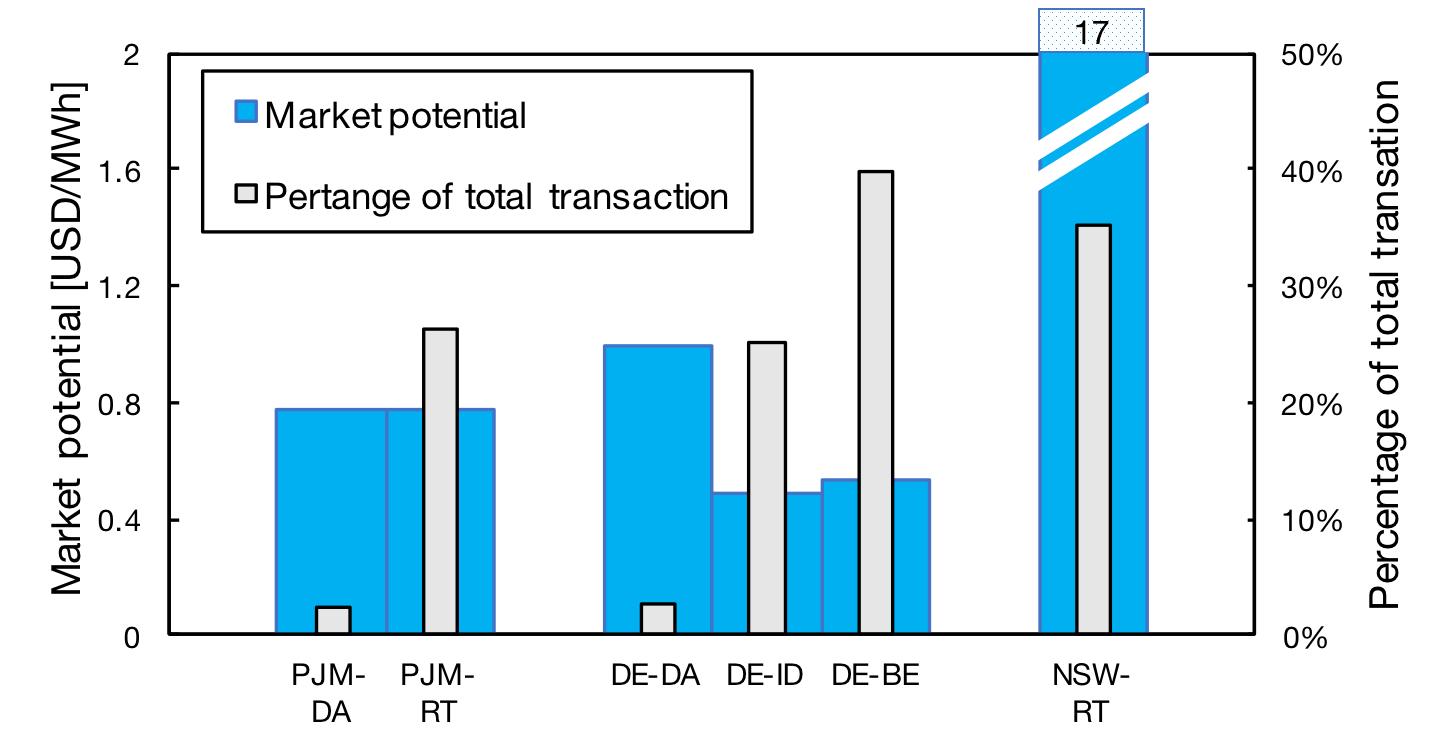
\includegraphics[width=0.95\linewidth]{Figures/Potential-Arbitrage}
	\caption{Market potential of arbitrage in energy markets using flexibility solutions}
	\label{fig:Potential-Arbitrage}
\end{figure}

By first focusing on the value in percentage of total transaction, we can observe clear distinctness between the day-ahead market  and the intra-day/ real-time/ balancing markets. In the day-ahead markets in both PJM and DE, arbitrage can capture only 2-3\% of the total transactions, where percentages are one order of magnitude higher, i.e. 20-40\% in other markets. This implies that even with irregularly large scales of flexibility resources, impacts on day-ahead market are still insignificant. In the real world, considering the competitions against established players, day-ahead market might not be an ideal marketplace for flexibility solutions. The reason for such a difference between different marketplaces can be explained by Table \ref{tab:price-3-geo}. %The NSW real-time market and DE balancing energy prices are highly volatile, corresponded to the 
%One may notice that ID and RT DA , 
As we can see, volatility reflected by standard deviation and amplitude of price movements raise significantly when the operation of market is close to real-time, and the market potential of arbitrage is highly dependent on the price volatility.

\begin{table}[h!]
	\footnotesize
	\centering
	\begin{tabular}{L{3cm} |R{1cm} R{1cm}| R{1cm} R{1cm} R{1.3cm}| R{1cm}}
		\hline
		& \multicolumn{2}{c|}{\textbf{PJM}}& \multicolumn{3}{c|}{\textbf{DE}}& \multicolumn{1}{c}{\textbf{NSW}}\\
		& DA & RT & DA &ID & BE &RT \\
		\hline
		Average price & 30.0 & 27.6 & 34.8 & 35.1 &40.7 & 46.0 \\
		Standard deviation & 11.6 & 14.8 & 15.0 & 16.1 &837.4 & 86.0 \\
		Maximum amplitude &121.2 &284.3&282.2&324.1&\num{1572.1}&9124.7\\
		\hline
		\multicolumn{7}{r}{in USD/MWh}
	\end{tabular}
	\caption{Price profiles in energy markets in the three cases}\label{tab:price-3-geo}
\end{table}

However, it should also be noted that price with higher volatility is less predictable, which in turn becomes an adversity for arbitrageurs. This issue will be discussed in the sensitivity study in Section \ref{sec:sensitivity} where we will analyze the effects of price foresight.

In terms of value in USD/MWh, it is particularly high in NSW's real-time market being 17 USD/MWh, while the values in other marketplaces are much smaller, around 0.4-1.0 USD/MWh. This is mainly because the Australia' NEM settles all transactions in the real-time market. Therefore, high price volatility due to real-time operations impacts all bulk electricity transactions. Such a market dynamics is more appealing than in the other two regimes. In fact, it is the philosophy of market design to fully exploit the ability of real-time energy market to response to the system imbalances which are otherwise tackled by frequency control markets\cite{AEMO2010}\cite{McConnell2015}. 

Finally, we list the original results in USD/yr which indicate the estimated market potential in each regime without normalization. It shows that the total market potentials for arbitrage in all three case happen to be slightly over 1 bUSD/yr. However, considering the overall scale of the power market, NSW should be the most attractive region among the three for business of flexibility solutions as has been mentioned above.

\begin{table}[h!]
	\footnotesize
	\centering
	\begin{tabular}{R{1cm} R{1cm} R{1cm}| R{1cm} R{1cm} R{1.3cm} R{1cm}| R{1cm}}
		\hline
		 \multicolumn{3}{c|}{\textbf{PJM}}& \multicolumn{4}{c|}{\textbf{DE}}& \multicolumn{1}{c}{\textbf{NSW}}\\
		 DA & RT & Total & DA &ID & BE & Total &RT \\
		\hline
		599 & 594 & 1194 & 515& 255 & 279 & 1049 & 1196\\
		\hline
		\multicolumn{8}{r}{in mUSD/yr}
	\end{tabular}
	\caption{Market potential for arbitrage in energy markets in non-normalized values}\label{tab:arbitrage-total}
\end{table}

In conclusion, flexibility solutions are not likely to play an important role in the day-ahead market. Instead, it should be of more significance in the market closer to real-time operations. NSW's real-time market that combines the attribute of large volume as in other day-ahead markets and high volatility in other real-time markets has the highest potential among the cases we have studied.


\subsubsection{Frequency control in ancillary service markets}

Figure \ref{fig:Potential-FC} illustrates the results for providing frequency control services in PJM and DE. The case of NSW is not studied due to data availability; referring to Appendix \ref{sec:accounting-data-prepare}. 

\begin{figure}[h!]
	\centering
	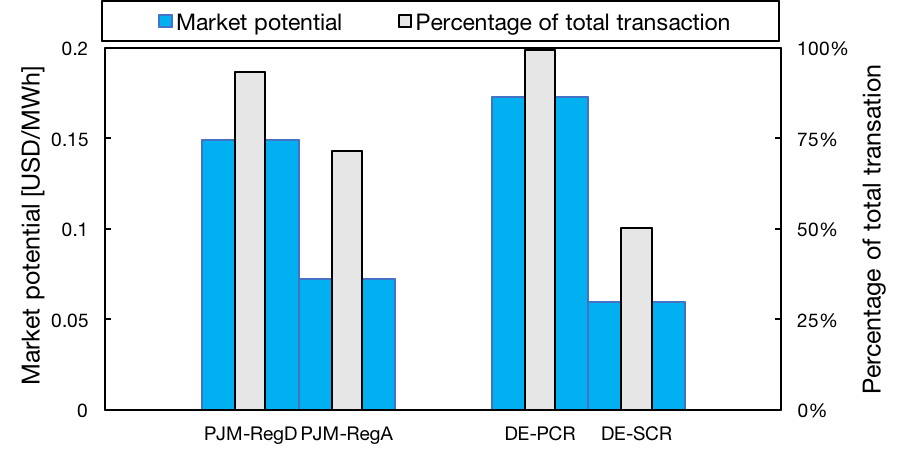
\includegraphics[width=0.95\linewidth]{Figures/Potential-FC}
	\caption{Market potential of frequency control in ancillary service markets using flexibility solutions}
	\label{fig:Potential-FC}
\end{figure}

Firstly, all for different marketplaces in two regimes have roughly the same level of potential, being 0.06-0.17 USD/MWh, which are about one order of magnitude smaller than the ones for arbitrage. This is in line with their comparative scale in general that large amount of transactions are made through energy markets.

What is more interesting is the value in percentage that reveals the accessibility of flexibility solutions to the frequency control markets. As we can see, the PCR that is made to have zero control signal as explained earlier in Section \ref{sec:data-parameter} (also referring to Appendix \ref{sec:accounting-data-prepare}), can be viewed as a control group and is shown to be fully accessible by our pre-defined flexibility solution. 

In contrast, we use actual control signals for RegD and RegA in PJM. The RegD that is specifically designed for emerging technologies with conditional energy-neutral signal indeed has a high accessibility, with over 93\% of its capacity can be supplied by our defined flexibility solution. RegA is not energy-neutral, but PJM allows frequency control services providers to make offer in hourly block, which offers great operationality for flexibility resource owners so about 70\% percentage of services can be covered by our solution. 

The SCR in Germany is a counter example, where offers have to be made in weekly peak/ off-peak blocks. Sustaining a service provision for such a prolonged duration is a challenging issue for the emerging flexibility technologies as explained in Section \ref{sec:neutral}. Even for the system in our study that is made to have ``ample size", it is only able to absorb or surplus energy in the grid, i.e. providing down regulation, while up regulation services is almost inaccessible since our system is not generating additional energy than what have been absorbed. It can be conceived that for real system without ``ample size" providing down regulation by constantly absorbing energy should also be an issue since the storage capacity will probably be exhausted.

This result verifies our hypothesis that non-energy-neutral signals will be a technical barrier for emerging flexibility solutions.

Further to what have been discussed in Section \ref{sec:neutral}, we tested the method to use third-party energy to self-neutralize the signal. In order to achieve this, we stack the operation of day-ahead arbitrage and providing frequency control service. In this way, the day-ahead energy is introduced to offset the frequency control signal. The results are depicted by Figure \ref{fig:Nuetralize}.

\begin{figure}[h!]
	\centering
	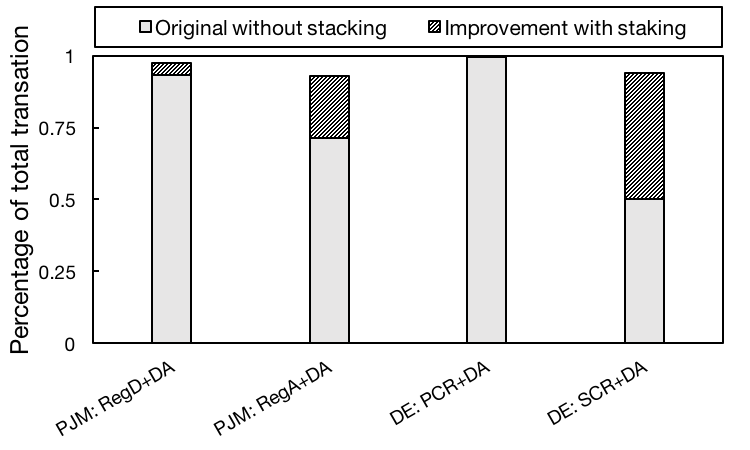
\includegraphics[width=0.95\linewidth]{Figures/Neutralize}
	\caption{Changes on accessibility by self-neutralizing the frequency control signals using energy from day-ahead market}
	\label{fig:Nuetralize}
\end{figure}

It is illustrated that with neutralized signal, the accessibility to all marketplace has been improved significantly. The percentages of covered capacity using our solutions have all exceeded 93\%. This demonstrates that the issue of non-energy-neutral signal is indeed a hurdle for flexibility solutions. Although the self-neutralization is shown to be a solution for the issue, in reality when the system size is always limited, certain amount of capacity is required to spare for tackling third-party energy, which obviously increases the operational complexity and may lead to lower profitability.

Finally, market potentials as annualized total revenues are provided as an additional reference for technology vendors in Table \ref{tab:fc-total}. Although we have seen a high percentage of value in this market can be captured, it is bounded by the overall market size of ancillary services which is relatively limited compared to the energy market.

\begin{table}[h!]
	\footnotesize
	\centering
	\begin{tabular}{R{2cm} R{1cm} R{1cm} R{1cm}| R{1cm} R{1cm} R{1cm}| R{1cm}}
		\hline
		&\multicolumn{3}{c|}{\textbf{PJM}}& \multicolumn{3}{c|}{\textbf{DE}}& \multicolumn{1}{c}{\textbf{NSW}}\\
		&RegD & RegA & Total & PCR & SCR & Total & FCAS \\
		\hline
		with staking &44.8 & 31.4&76.2&89.7&31.1&120.8& \multirow{2}{*}{\textit{23.4\footnote{Total market size without technical analysis}}} \\
		w/o staking & 46.7 & 40.8& 87.1&89.7& 58.1&147.8& \\
		\hline
		\multicolumn{8}{r}{in mUSD/yr}
	\end{tabular}
	\caption{Market potential in non-normalized values for providing frequency control services}\label{tab:fc-total}
\end{table}

To sum up, market potential for frequency control is smaller than energy arbitrage and emerging flexibility solutions may face technical difficulties to follow the control signal, if it is not designed to be energy-neutral.

\subsection[Profitability and market potential of energy storage]{Profitability and market potential of energy storage%}
	\sectionmark{Energy storage}}
\sectionmark{Energy storage}
	
In last section, the potential of value creation using flexibility in power markets has been verified. Especially for arbitrage in energy market, a vast market is being unlocked with explicit barrier being removed. For market players, a further question would naturally be how to realize that potential, i.e. which technologies should be employed.

In this section, we evaluate the battery energy storage system (BESS). Firstly, the profitability of BESS is examined with ``small size" of system as introduced earlier in Section \ref{sec:quant-case-setup}. Furthermore, if there is use-cases that show a positive profitability, we will further extend the system size to find the ``profitable size" which indicates a market potential for BESS only, compared to the market potential for flexibility solutions in general without considering the cost.

This section is organized by each regime and using historical electricity market data as input.


%\subsection{Valuation of markets under current market conditions}
%This section presents the results using historical market data. Since two types of technologies and markets in three geographies were studied, there are a total of six distinct setups with each comprises several use-cases. In addition, we included a cost break-even analysis specifically for ESSs as few profitable opportunities were found due to high costs on battery stocks.

\subsubsection{BESS profitability and market potential in PJM}

The profitability of BESS in PJM power markets with different use-cases are illustrated by Figure \ref{fig:pjm-ess-profitability}.

\begin{figure}[h!]
	\centering
	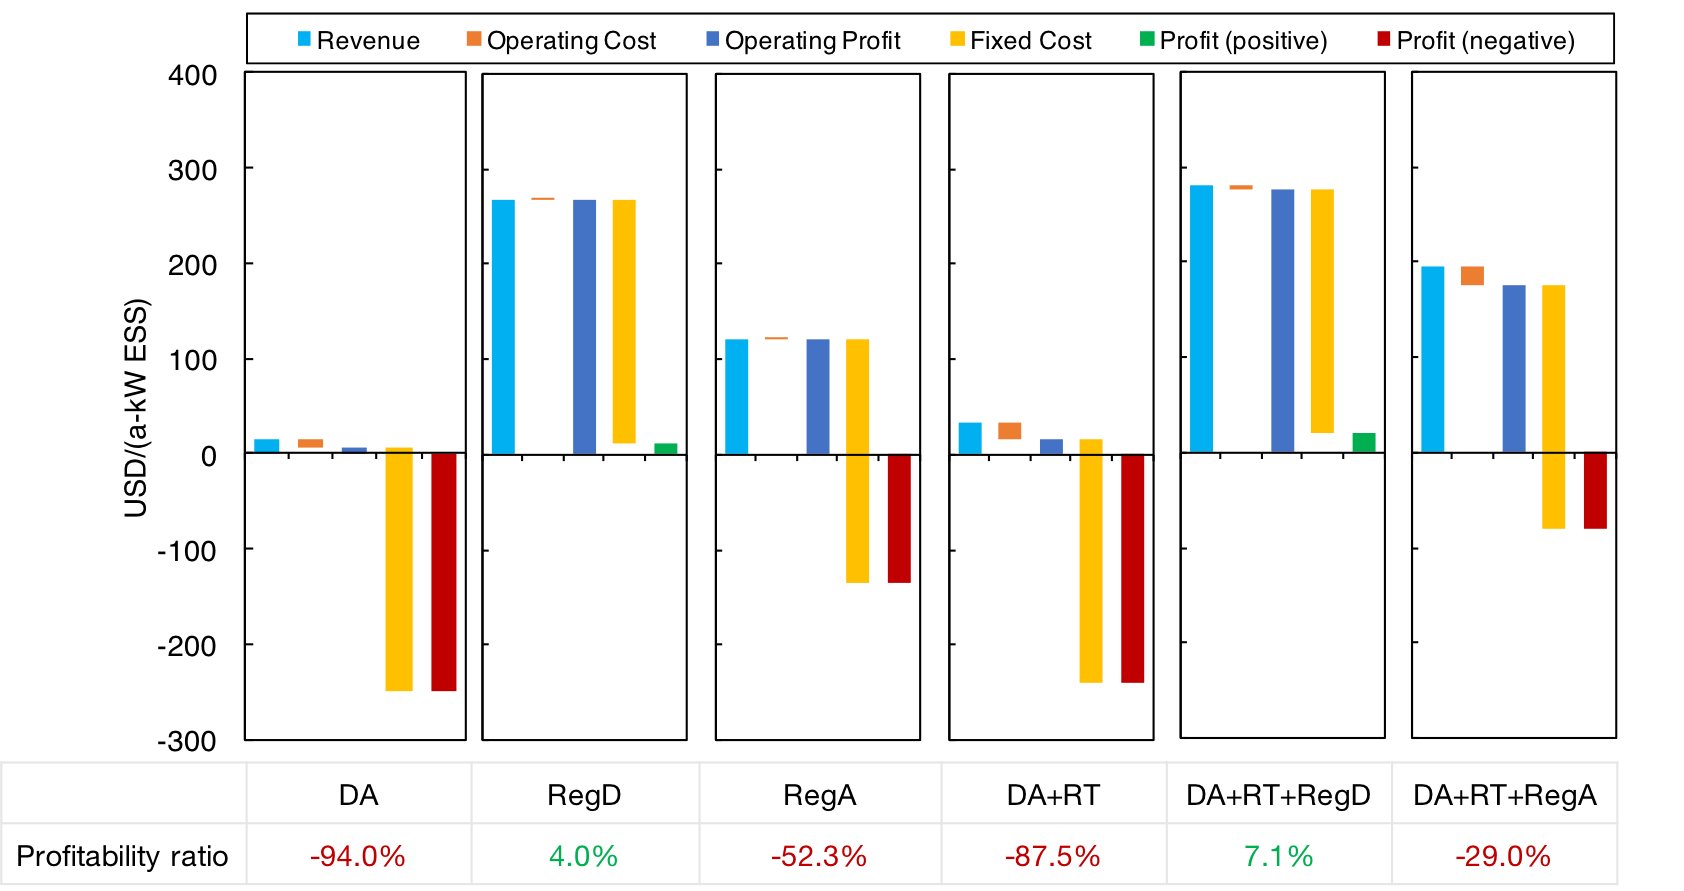
\includegraphics[width=0.9\linewidth]{Figures/PJM_ESS_profitability}
	\caption{Profitability of  BESS with ``small size" in PJM electricity markets}
	\label{fig:pjm-ess-profitability}
\end{figure}


As we can clearly see, the RegD marketplace that is specially designed for emerging flexible technologies is indeed profitable. This should give merit to PJM's RegD design including the conditional signal neutrality, operational flexibility, as well as higher price based on actual performance, as mentioned in Section \ref{sec:qualitative-analysis} (also referring to Appendix \ref{sec:accounting-data-prepare} for more details). Apart from RegD market, there are no other profiting opportunities existing in PJM, primarily due to the high fix cost that is nothing but the CAPEX spent on battery in our study. Even the conventional regulation service RegA will create losses to BESS players.

Direct participation of BESS in the energy market is a pending issue, but can be indirectly realized by behind-the-meter distributed storage and through PJM's DR program, as discussed in Section \ref{sec:qualitative-analysis}. However, it is not profitable at all. The revenue is very niche, which shall be explained by its relatively low energy price (as a result of shale gas revolution since 2008) and low volatility as we have seen in Table \ref{tab:price-3-geo} in last section. The volatility in energy market is lower than the other two regions, which can be explained by many reasons, including the relative lower penetration and the existence of capacity market that bypasses some value that would otherwise be reflected on energy markets.

Staking services to perform multitasking can improve the profitability slightly but does not flip over the profitability of any use-cases. 

Furthermore, we detect the ``profitable size" and compared it to the maximum potential using flexibility solutions in general to see how much of the market potential can be realized by BESS. Since none of other markets expected for RegD are profitable with ``small size", the ``profitable sizes" for those use-cases are therefore zero. In contrast, it is found that 100\% of the RegD market can be realized with positive profits.

In conclusion, BESS is not profitable in most use-cases in PJM due to the high CAPEX of batteries, together with relative low and stable energy price. However, the whole market for RegD frequency control product that is designed exclusively for emerging flexibility solutions is indeed profitable. 
%The market with a total size of 513 USD/$(\text{a} \cdot \text{MW})$ can be wholly materialized by 2 kW/(MW consumption) BESSs without writing a loss, although the margin is very niche, barely above zero; see Figure \ref{fig:pjm-ess-profitable-size}.

%Those merits allow BESS players to offer RegD alone without coupled operations in the energy market. As a result, stacking it with the energy market does not improve the profitability and tangible market size as significantly as in Germany. As we can see from an example shown by Figure \ref{fig:pjm-multitasking}, the system with pre-defined parameters in this study will have slightly surplus energy while strictly following the RegD signal. The SoC would raise quite slowly so that the resource can sustain the provision of RegD service over a long period (at least 84 hours shown in the chart) without involving transactions in energy markets. Trading in energy market is activated to leverage the arbitrage potential due to extreme price movements, which is however infrequent. Serving RegD is preferred for most of the time due its higher profitability. 

%\begin{figure}[h!]
%	\centering
%	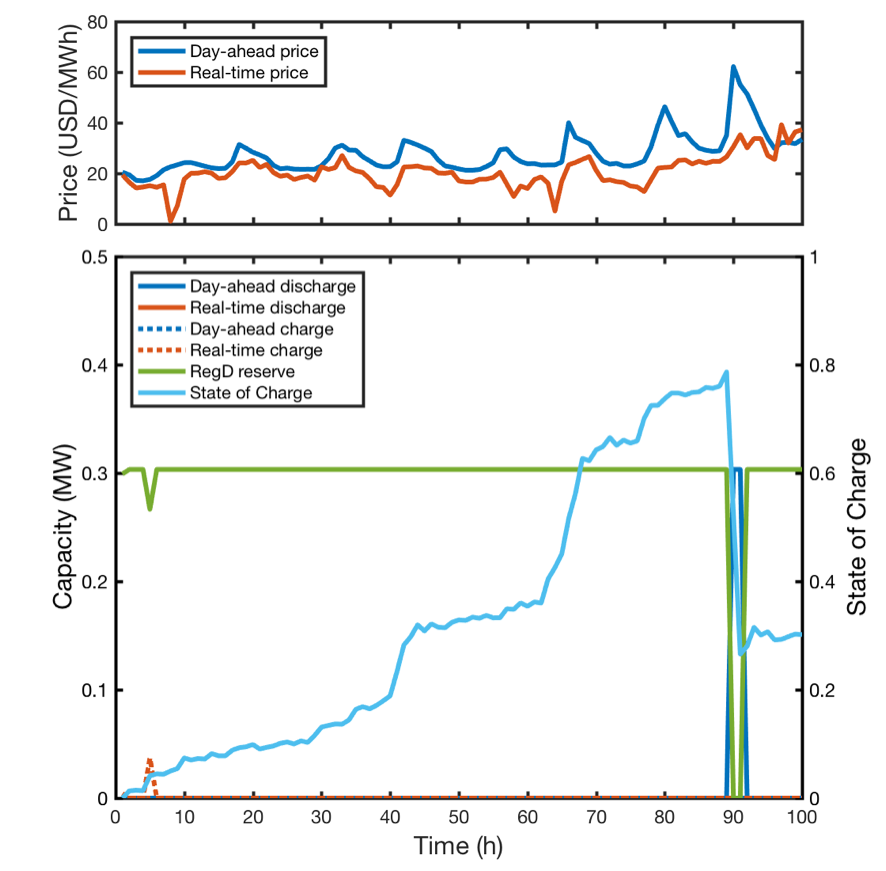
\includegraphics[width=0.9\linewidth]{Figures/PJM_multitasking_example}
%	\caption{A example of operational plan with a 0.3MW battery energy storage system}
%	\label{fig:pjm-multitasking}
%\end{figure}


%Overall, PJM shows a perfect example on how to offer incentives for the emerging storage technologies that are beneficial to the system, by implementing proper market frameworks such as the RegD and the  emergency DR program. For technology vendors, this market is already quite mature without spare space for new entrants unless significant changes may occur on market conditions, e.g. vast renewable penetration. Nonetheless, existing business cases in PJM may offer viable references for technology vendors to conduct similar practices in other markets. 
%The upper-bounded values indicating the market potential are summarized in Table \ref{tab:pjm-summary}.


\subsubsection{BESS profitability and market potential in DE}

Figure \ref{fig:germany-ess-profitability} summarizes the profitability of all use-cases in Germany's power markets. 

\begin{figure}[h!]
	\centering
	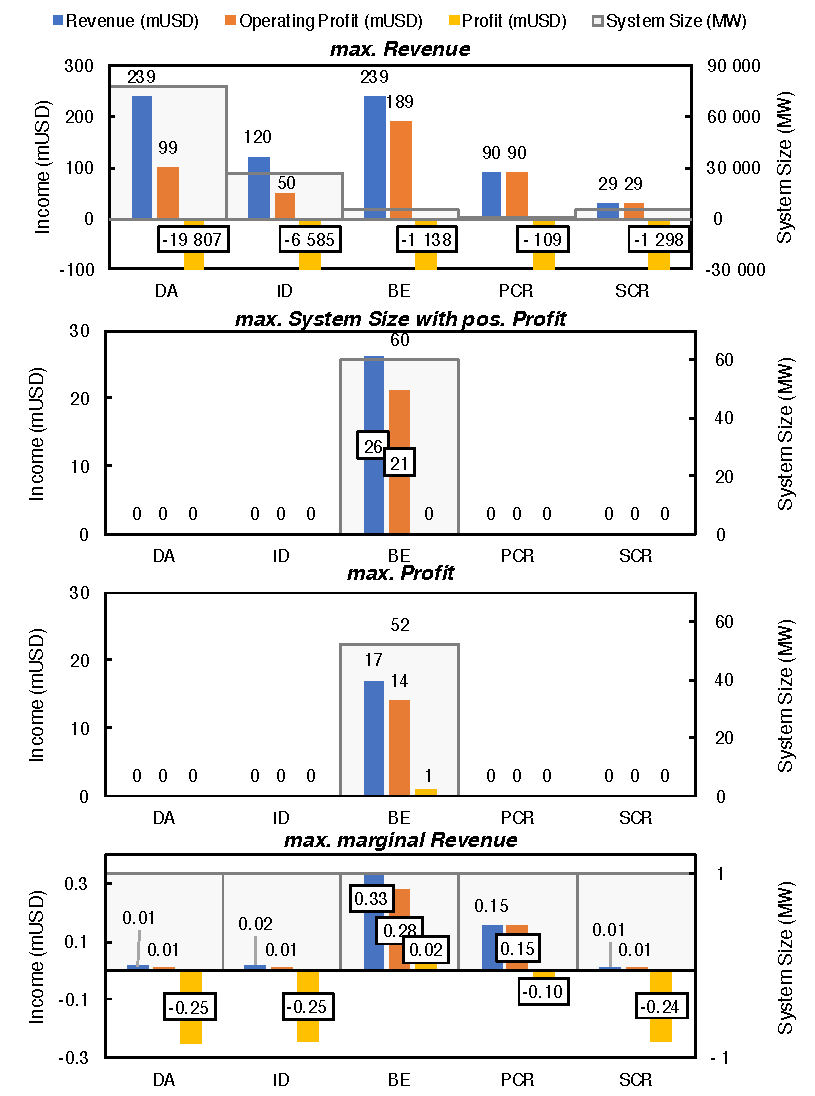
\includegraphics[width=0.9\linewidth]{Figures/Germany_ESS}
	\caption{Profitability of  BESS with ``small size" in DE electricity markets}
	\label{fig:germany-ess-profitability}
\end{figure}

%As is discussed, profitability analysis can be performed using the scenario ``max. marginal Revenue", the results of which are depicted by Figure \ref{fig:germany-ess-profitability}. By showing values per unit ESS system installed, we can see the maximum unit return of ESS in Germany power markets. 

%Meanwhile, with ample size of ESS, maximum potential market sizes can be derived, corresponding to the scenario ``max. Revenue".
%Summarized by Figure \ref{fig:germany-ess}, annual cash flows are shown per MW consumption as normilzed values to the overal average consumption, \num{59138} MW . For example, the normalized revenue for arbitrage in day-ahead market is \num{4041} USD per year per MW consumption, which indicates the achievable revenue for a power system in Germay with 1 MW average load and corresponds to 239 mUSD/a in whole German market by mutiplying the base of \num{59138} MW.

It was found that the only profitable case is delivering balancing energy for self-balancing of BGs. As we have seen previously in Table \ref{tab:price-3-geo}, the balancing energy price is extremely volatile due to the way how it is calculated as introduced in Section \ref{sec:quali-de}. However, such a volatile price is very hard to be predicted precisely, which is likely to abate the feasibility of performing arbitrage, as we will see in the sensitivity analysis. 

Besides, losses are seen for all the other use-cases. Apart from providing primary control reserve, revenues are almost negligible to fixed costs. Similar to the result in PJM, it again reveals the fact that battery cost is still too high to make a profitable business. 

Generally, providing frequency control should be more rewarding than energy arbitrage since there are higher prerequisites for resources to perform frequency control than merely to deliver energy. This applies for the result of primary control reserve PCR, but does not fit the case of secondary control reserve SCR. In previous section, we have argued although staking SCR with energy markets will make it fully accessible for flexibility solutions by self-neutralizing the control signal, it is not likely to be profitable as part of the capacity needs to be reserved for energy transaction rather than committed to frequency control markets. This is verified in the results, staked with energy markets, the profitability of SCR is still deeply negative and not comparable to PCR that is with a zero control signal in our study.

It is actually an interesting finding to see that providing frequency control services are less profitable than providing self-balancing services to BGs, considering the fact that the balancing energy arrangement is used a way to partially recover the costs that TSOs spent in stabilizing the frequency. The profits in serving balancing energy means the costs of using BESS is lower than the partial costs incurred to TSOs. However, BESS is not favored in the gateway where TSOs procure the frequency control services. This actually a strong implication that TSOs should consider options to modify the framework in frequency control services in order to enable more flexibility solutions. Nevertheless, it is not our primary focus that advising the market designers.

We further investigated the profitable size of providing balancing energy service, and found only 9\% of the total potential we concluded for flexibility solutions in general in last section, that is equal to 0.05 USD/MWh, would be profitable for BESS, which is not likely to attract many market players.


%As is analyzed in Section \ref{sec:qualitative-analysis}, this case corresponds to the situation of self-balancing where the players turn to the flexibility resource in avoidance of charges by TSOs for their imbalances. We further analyzed the maximum profitable system size and maximum profit of using the pre-defined BESSs; see Figure \ref{fig:germany-ess-profitable-size}.

%\begin{figure}[h!]
%	\centering
%	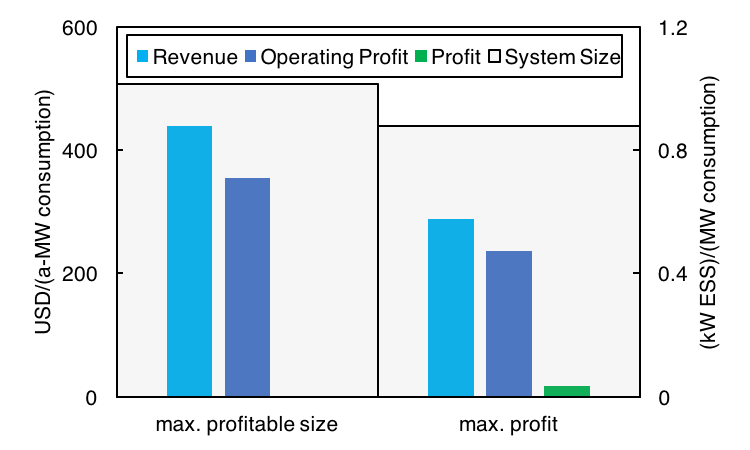
\includegraphics[width=0.9\linewidth]{Figures/Germany_ESS_profitable_size}
%	\caption{Market size of ESS in Germany electricity markets in the scenario of ``max. System size with pos. Profit" and ``max. Profit"}
%	\label{fig:germany-ess-profitable-size}
%\end{figure}

%It can be seen from Figure \ref{fig:germany-ess-profitable-size}, if being operated optimally BESSs with a size of up to 1 kW/(MW consumption) can generate profits by serving balancing energy, corresponding to a total 60MW in Germany. Nevertheless, it is challenging to be realized in practice. Market players do not have the right information to optimize their operational plans, since the balancing energy price, reBAP, is calculated \textit{ex-post} and highly volatile, hardly predictable, as is discussed in Section \ref{sec:qualitative-analysis}. On the contrary, if a system is designed to have ample size and tackle almost all imbalance events, it corresponds to a situation as the ``max. Revenue" scenario where we see negative profits from Figure \ref{fig:germany-ess-profitability}.

%On the other hand, we noticed from Figure \ref{fig:germany-ess-profitability} that selling frequency control services to TSOs is less economically viable than using BESSs for self-balancing.The maximum marginal revenue from self-balance is significantly higher (33 times) than from selling frequency control products, while ideally the situation shall be reversed. The balancing energy charges are designed to recover the costs of activating frequency control services (calling for energy delivery) while the costs paid for securing capacity commitment are socialized, as have been fully discussed in Section \ref{sec:qualitative-analysis}. Theoretically, players shall get higher turnover in the frequency control markets than avoided balancing energy charges. Furthermore, the actual total payment for SCR in Germany is 176 mUSD in 2016 which is equavilent to \num{2976} USD/$(\text{a} \cdot \text{MW})$, while the maximum achievable revenue with BESSs are bounded at \num{490} USD/$(\text{a} \cdot \text{MW})$ as shown in Figure \ref{fig:germany-ess} with the rest 83.5\% of the market is intangible for BESSs . Our results imply that the current design of frequency control markets is neither economically efficient nor technically feasible to integrate the emerging BESS resources, which verifies our analysis in Section \ref{sec:qualitative-analysis}. We have argued that hurdles exist against emerging BESS to participate in frequency control markets with the non-energy-neutral signals and block-wise offering, especially for SCRs which demand significantly higher energy delivery than PCRs.

%Facing either lack of information transparency in balancing energy charges or unfavorable market rules in frequency control markets, BESS players have no feasible options in the current market setup to make profits.

%However, we may argue this situation shall not be long-lasting. We have already seen that certain amount of BESS will be a cheaper option to defer the expense on imbalance settlements compared to what are currently incurred. The market operators shall develop well-designed frameworks to encourage the participation of these resources that are beneficial to lower the overall system costs. In reality, there are indeed debates proposing possible solutions on this issue, e.g. letting TSOs who have the most abundance of information own and dispatch the storage resources\cite{He2012}, re-engineering the pricing mechanism of balancing energy\cite{Wartsila2014} and implementing favorable frequency control products for storage\cite{Megel2017}, etc.

%As an implication for technology vendors, these possible movements on market designs shall be taken care of as it could suddenly turn over the feasibly profitability of using BESSs for balancing services.

%Regarding arbitrages value in energy market, although the potential revenues are \num{4041} USD/$(\text{a} \cdot \text{MW})$ in day-ahead and \num{2029} USD/$(\text{a} \cdot \text{MW})$ in intra-day market, the losses would be incredibly high in order to materialize the revenue using BESSs; see Figure \ref{fig:germany-ess}. Even in the scenario of maximum unit return, the losses are about 10-20 times of the revenue; see Figure \ref{fig:germany-ess-profitability}. It is clear that the heavy investments on batteries cannot be recovered from making arbitrage in energy market. However, since the operating profits are always positive, if technology vendors can enable similar functions as BESS using technologies with smaller capital costs such as certain types of DR, it is still possible to make profits out of the market worth a total of over 300 mUSD per annum in Germany.

%\begin{figure}[h!]
%	\centering
%	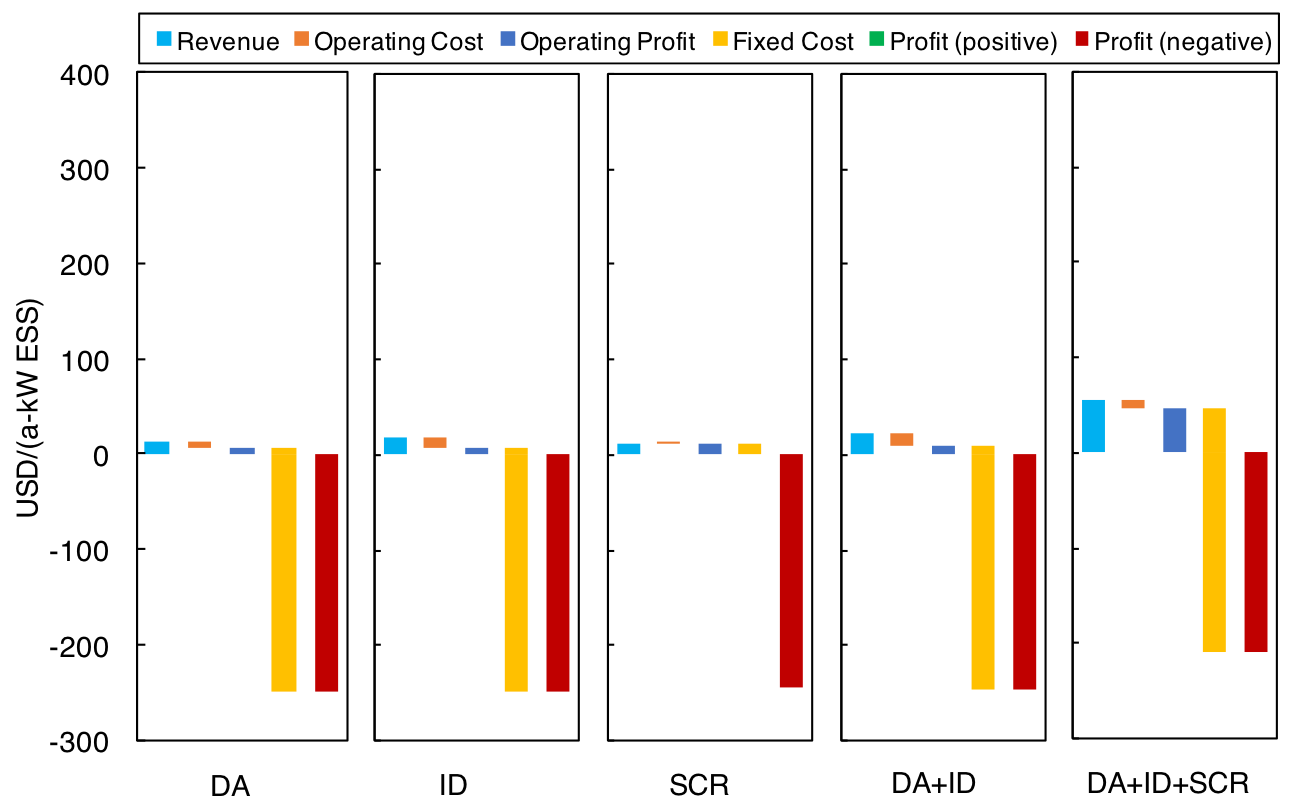
\includegraphics[width=0.95\linewidth]{Figures/Germany_ESS_profitability_multitasking}
%	\caption{Profitability of ESS with multitasking in Germany electricity markets}
%	\label{fig:germany-ess-multitasking-profitability}
%\end{figure}

%\begin{figure}[h!]
%	\centering
%	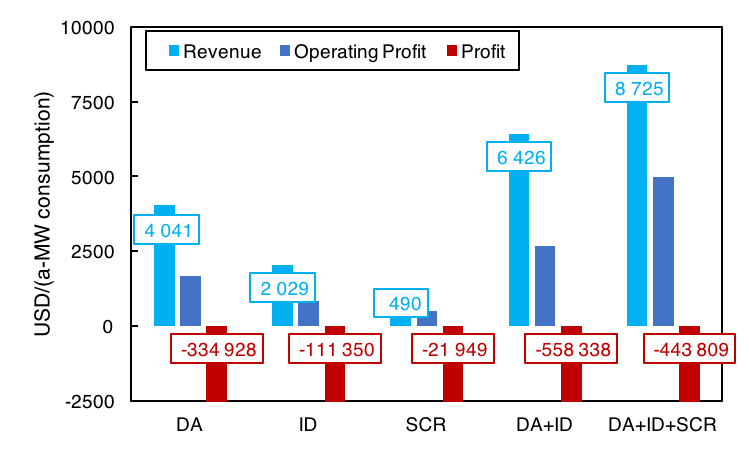
\includegraphics[width=0.95\linewidth]{Figures/Germany_ESS_multitasking}
%	\caption{Market size of ESS with multitasking in Germany electricity markets}
%	\label{fig:germany-ess-multitasking}
%\end{figure}

%As has been discussed qualitatively, in order to increase the profitability and find a way to neutralize the frequency control signals, we may stack operations in day-ahead, intra-day and secondary control reserve for multitasking. Figure \ref{fig:germany-ess-multitasking} shows the effects of multitasking.

%While there are no significant synergies observed between day-ahead and intra-day markets (the unit returns remain unchanged in the scenario of maximum marginal revenue), stacking secondary control reserve with these two energy marketplaces will significantly improve the unit revenue (from 11 and 22 USD/$(\text{a} \cdot \text{MW})$ to 54 USD/$(\text{a} \cdot \text{MW})$) as well as the maximum revenue potential (from \num{6426} USD/$(\text{a} \cdot \text{MW})$ plus \num{490} USD/$(\text{a} \cdot \text{MW})$ to \num{8725} USD/$(\text{a} \cdot \text{MW})$). The maximum unit operating profit, as a consequence, raises by 4.5 times. The increment of maximum potential revenue of \num{2299} USD/$(\text{a} \cdot \text{MW})$ by stacking SCR on DA+ID indicates an additional revenue of \num{1809} USD/$(\text{a} \cdot \text{MW})$ are accessible for ESS in the SCR markets, reducing the intangible part from 83.5\% to 22.7\%. This corresponds to our previous analysis that the non-energy-neutral signal is indeed an issue for BESSs and has to be neutralized externally. Nonetheless, coping with third-party energy transactions requires the BESSs spare certain capacity to receive or release the energy, which reduces their availability in delivering SCR services. This is reflected on the result that this case with multitasking is still not profitable.

%To sum up, while arbitrage is mainly constrained by costs on the technology side, making profits from balancing services is limited by adverse market frameworks although it has already shown its ability to make a positive contribution to the system. Technology vendors shall consider other technologies than BESSs or expect drastic cost reduction of BESSs to unlock the arbitrage value worth over a total of 300 mUSD/a in Germany. Profits from balancing market are more technically tangible, yet adjustments on market frameworks are required.

To sum up, without a special arrangement like the RegD market in PJM, there are not really opportunities in Germany for players to make profits. Delivering balancing energy seems to be an option. However, it is purely benefited from the high price volatility, together with the perfect foresight we assigned to them in our study. Nevertheless, the comparison of profitability between avoiding balancing energy charges and providing frequency control services reveals the merits of BESS are not fully embraced by TSOs. As a result, improvements on the rules could be expected.


\subsubsection{BESS profitability and market potential in NSW}

In the previous section, we have shown that the real-time market has the highest potential for arbitrage. Hereby, we further evaluated its profitability, as shown in Figure \ref{fig:nsw-ess-profitability}.
%In New South Wales power markets, we only studied the real-time energy market, which was primarily due to the limitation of data availability.  Only information about total payment are available for the frequency control products. However, it was found that the overall size of these unaddressed markets are indeed negilible compared to the real-time energy market. The total payment in NSW's frequency control ancillary service (FCAS) market was worth 23.4 mUSD (2933 USD/$(\text{a} \cdot \text{MW})$) in 2016, which was equal to just 0.53\% of the total payment in the real-time energy market that was 4.4 bUSD (\num{551516} USD/$(\text{a} \cdot \text{MW})$). It was also much smaller than merely the arbitrage value, being 2.7\% of the revenue from arbitrage of \num{109301} USD/$(\text{a} \cdot \text{MW})$ as shown by Figure \ref{fig:nsw-ess}. This reflects the philosophy of market design to fully exploit the ability of real-time energy market to response to the system imbalances which are otherwise tackled by frequency control markets\cite{AEMO2010}\cite{McConnell2015}.
%As a result, the price volatility in NSW's real-time energy market is significantly higher than the energy markets in other geographies, as is shown by Table \ref{tab:price-3-geo}.

\begin{figure}[h!]
	\centering
	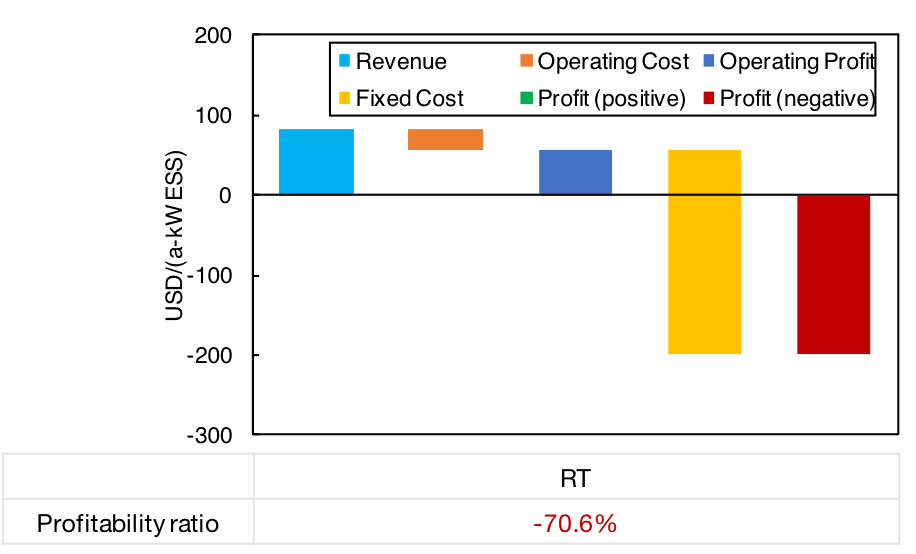
\includegraphics[width=0.8\linewidth]{Figures/NSW_ESS_profitability}
	\caption{Profitability of  BESS with ``small size" in NSW electricity markets}
	\label{fig:nsw-ess-profitability}
\end{figure}

It is shown that even though in such a volatile real-time energy market, it is still not a profitable business to deploy BESS in NSW for arbitrage. Although the profitability ratio being -70.6\% is much better than values in energy markets in the other two regimes. 
%Such a volatile market is favorable for arbitrage. As we can see from Figure \ref{fig:nsw-ess-profitability} and \ref{fig:nsw-ess}.Profitability-wise the marginal revenue per unit system, 83 USD/$(\text{a} \cdot \text{kW ESS})$) is 2.4 times the value of arbitrage in DA+RT in PJM and 3.8 times the value of arbitrage in DA+ID in Germany. In terms of market potential, the maximum arbitrage revenue \num{109301} USD/$(\text{a} \cdot \text{MW})$) is roughly 17 times higher compared to either of those two arbitrage cases in Germany and PJM.
~\newpage
\subsubsection{Cost reduction: where is the break-even point for arbitrage using BESSs}

According to the results above, there are almost no profitable opportunities for BESS.  Providing frequency control should be more promising as the situation could be improved by market re-structuring. This is successfully demonstrated by the example of PJM's RegD design, and we have saw rationale to motivate the market designer go for a similar approach in Germany.

The value of arbitrage, however, is far away from being profitable due to high expenses on batteries. Overturn of arbitrage profitability using BESSs has to rely on reducing costs and changing market conditions. While the latter will be discussed in the proceeding section, hereby we present the results with reduced costs of battery stocks. 

In each regime, the case with the highest arbitrage potential was selected, which is respectively arbitrage in coupled day-ahead and intra-day market in Germany (DA+ID), arbitrage in coupled day-ahead and real-time market in PJM (DA+RT), arbitrage in real-time market in NSW (RT). We would show the maximum profitability ratio that is realized by a small size of BESS. Meanwhile  we would present the ratio between the  profitable revenue that is obtained as in the scenario of ``profitable size" to the maximum potential revenue derived from ideal flexibility system with ``ample size". 

\begin{figure}[h!]
	\centering
	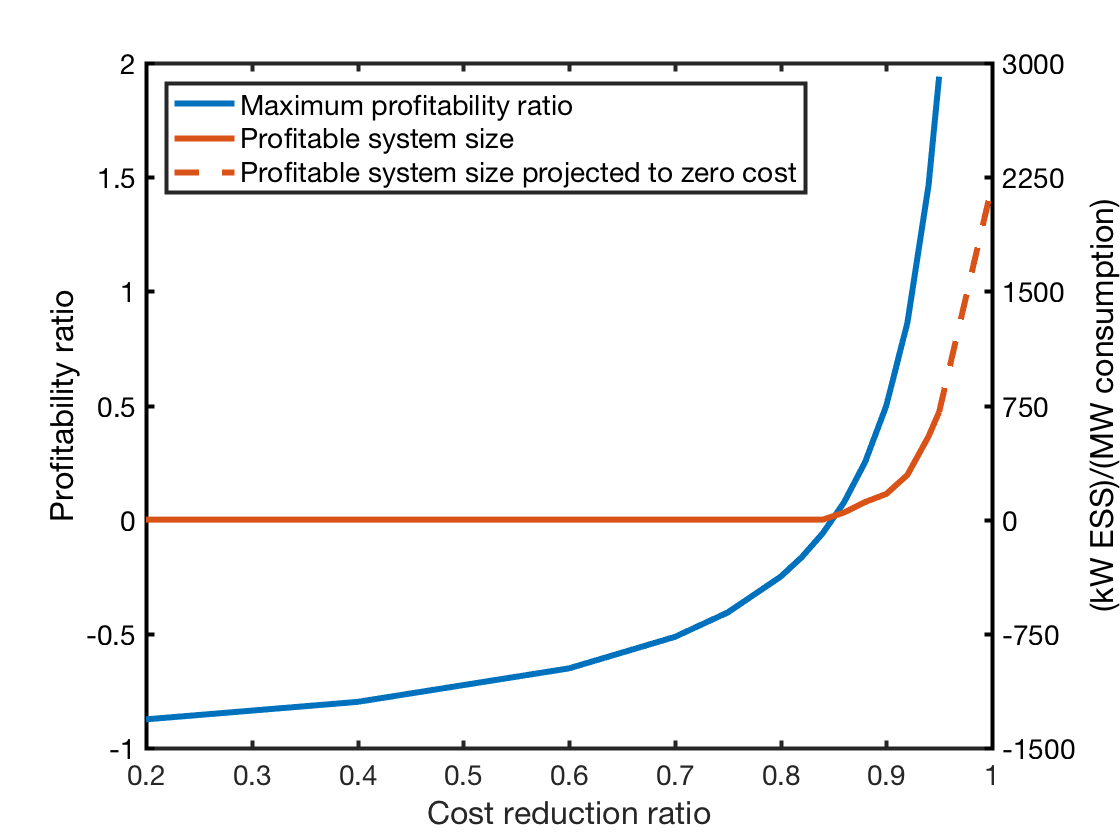
\includegraphics[width=0.9\linewidth]{Figures/CostReduction_Germany_ESS}
	\caption{Development of market size and profitability of arbitrage in coupled day-ahead and intra-day markets with reduced costs in Germany}
	\label{fig:germany-ess-costreduction}
\end{figure}

\begin{figure}[h!]
	\centering
	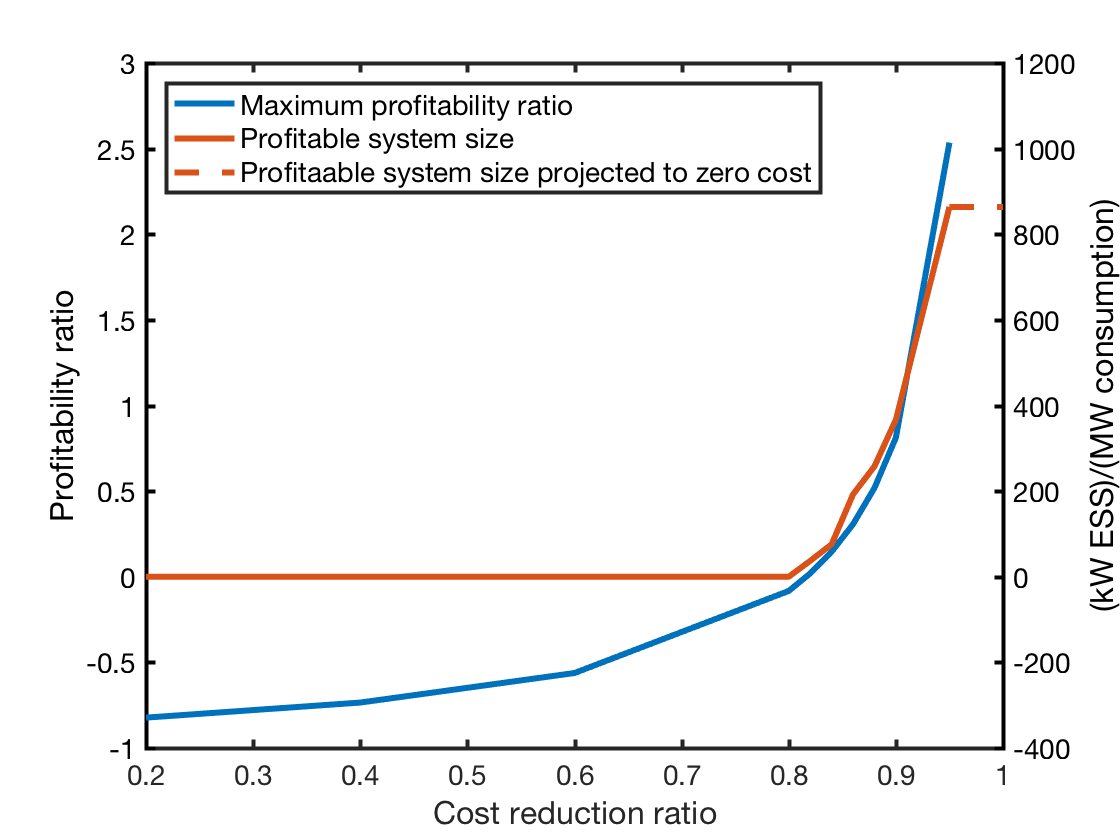
\includegraphics[width=0.9\linewidth]{Figures/CostReduction_PJM_ESS}
	\caption{Development of market size and profitability of arbitrage in coupled day-ahead and real-time markets with reduced costs in PJM}
	\label{fig:pjm-ess-costreduction}
\end{figure}

\begin{figure}[h!]
	\centering
	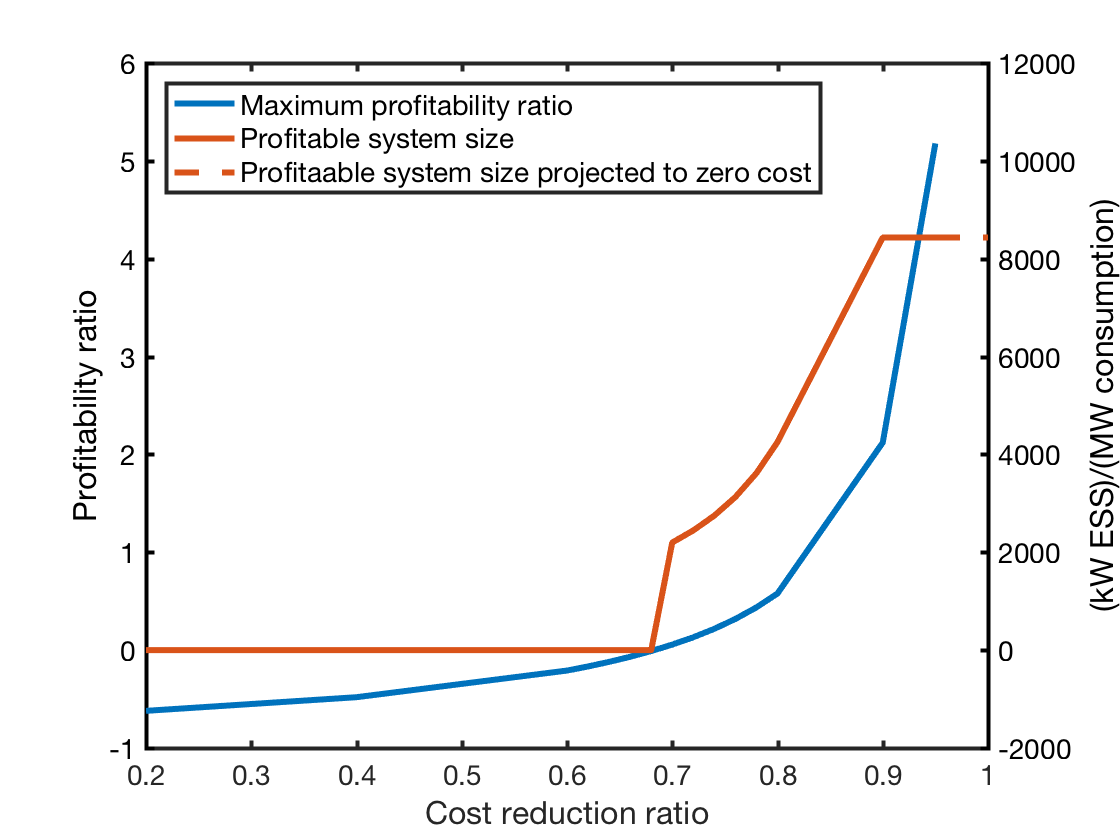
\includegraphics[width=0.9\linewidth]{Figures/CostReduction_NSW_ESS}
	\caption{Development of market size and profitability of arbitrage in real-time markets with reduced costs in NSW}
	\label{fig:nsw-ess-costreduction}
\end{figure}

Figure \ref{fig:germany-ess-costreduction} - \ref{fig:nsw-ess-costreduction} illustrate how the profitability and market size will evolve with cost reduced by up to 95\% in three geographies. The break-even point of costs is found to be 84\%, 81\% and 68\%, respectively in Germany, PJM and NSW. If we adopt the forecast made by IRENA\cite{IRENA2017} who predict the cost reduction by up to 60\% by 2030, none of these markets will be profitable for arbitrage by 2030. Even if we applied a constant learning rate of 14\% per annum according to \cite{Nykvist2015}, the break-even point will be realized in 12, 11 and 8 years, respectively in Germany, PJM and NSW. 

Moreover, it shall be noticed while the break-even point is just reached, the total profitable revenue will be almost at zero. To materialize the whole potential of arbitrage revenue, it requires a cost reduction of 95\%+, 95\% and 90\%, respectively in Germany, PJM and NSW, which is almost impossible to be realized in the foreseeable future.

As a conclusion, the cost reduction of BESS by learning effect alone will not turn over the profitability of arbitrage using BESSs in the near future. Unless revolutionary technical innovations happen, opportunities of arbitrage using BESS may only arise with drivers from the market, e.g. renewable penetrations, which are to be shown in Section \ref{sec:impact-market-condition}.
\subsection[Profitability and market potential of electric vehicle to grid]{Profitability and market potential of electric vehicle to grid%}
	\sectionmark{Electric vehivle to grid}}
\sectionmark{Electric vehivle to grid}

EV is taken as a representative of demand response technologies. As elaborated when introducing the methodology in Section \ref{sec:tech-simulation-module}, we have pointed out that implementing EV as a grid resource is not as straightforward as using ESSs, with the issues of uncontrolled users' behavior as well the energy demand of the resources themselves.  

In fact, EV charging itself is a challenge to grid. It is not possible to deliver any services without incorporate a large-volume energy market to fulfill energy consumed for drivings. 

Therefore, the day-ahead energy market is always included for all the cases for EV2G. Moreover, in our case studies, it is found even with the day-ahead market, charging the EVs is not feasible while their number reached a certain level. In the optimization framework, the market liquidity constraints would be violated, especially the one that we set to restrict the activation of peak generation during non-peak hours, while the EV fleet grows beyond a certain scale. This corresponds to the situation where spare generation resources in the power system are not sufficient  to fulfill the energy needs of EVs. The electricity price may raise significantly in those scenarios compared to nowadays's level.

Taking the case of DE as an example, Figure \ref{fig:EV_nan_percentageg} shows the percentage of time within a year when the charging demand cannot be well fulfilled without activating more peak generation, even using EV2G technology to optimize the charging behavior.

\begin{figure}[h!]
	\centering
	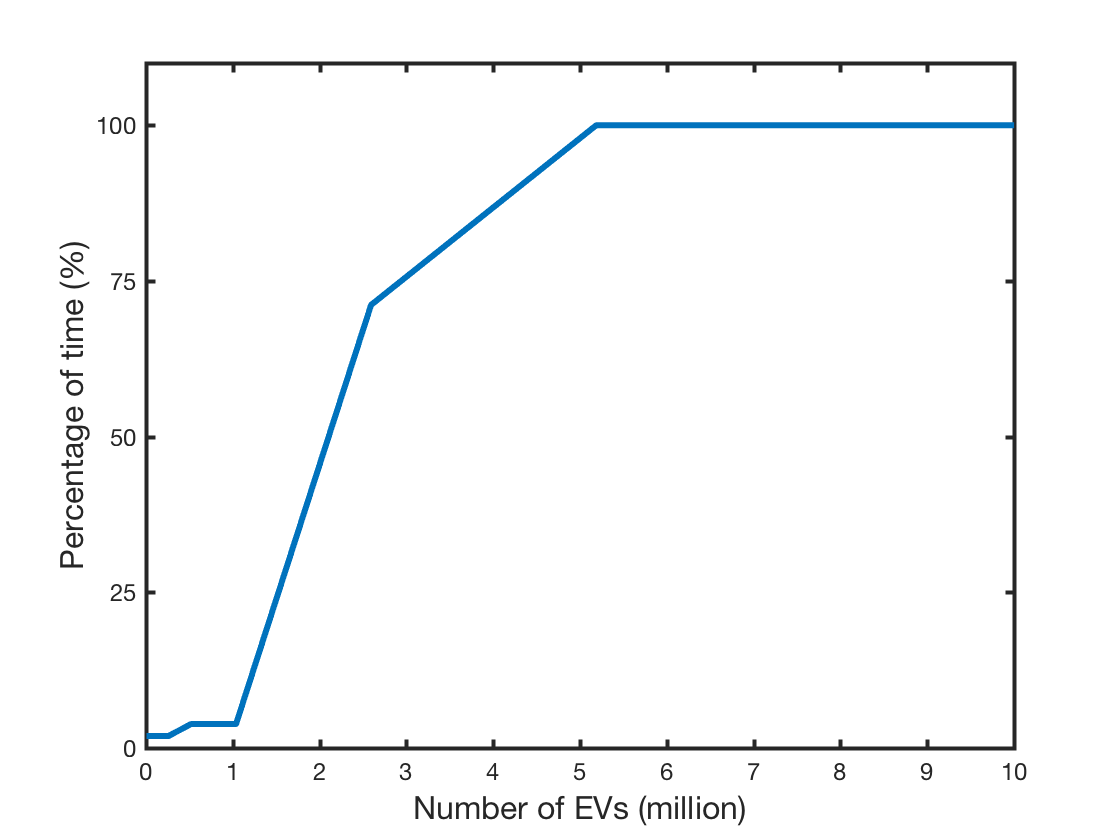
\includegraphics[width=0.95\linewidth]{Figures/EV_nan_percentage}
	\caption{Percentage of time when EV charging demand cannot be fulfilled in Germany}
	\label{fig:EV_nan_percentageg}
\end{figure}

We can see when the number of EV is higher than 1 million, it start to stress the electricity supply if the generation capacity remains at present level. 

This finding implies when there will be 1 million more EVs in Germany compared to the number in 2016, it will create great incentives for infrastructure extension of electricity grid, which reveals a promising business opportunity. Nevertheless, studies under that condition is beyond the focus of our work. Instead, we would only perform scenario analysis when the number of EV is within the limit of 1 million. 

In our study, we carefully check this issue and make sure that the infeasibility of fulfilling charging demand will not happen. The scenario of ``2\% market share", e.g. with 0.9 million EV in Germany, is actually close to the critical point in all three cases, which indicates a soft up bound of EV2G potential without grid infrastructure upgrade. 

Finally, we performed the case studies based on scenarios described earlier in Section \ref{sec:quant-case-setup} and results are presented by each regime.

\subsubsection{EV2G profitability and market potential in PJM}

Figure \ref{fig:PJM_EV} summarizes the results of use-cases in PJM. Arbitrage in day-ahead market only is not profitable. Coupled operations in real-time market lead to niche profits. 

\begin{figure}[h!]
	\centering
	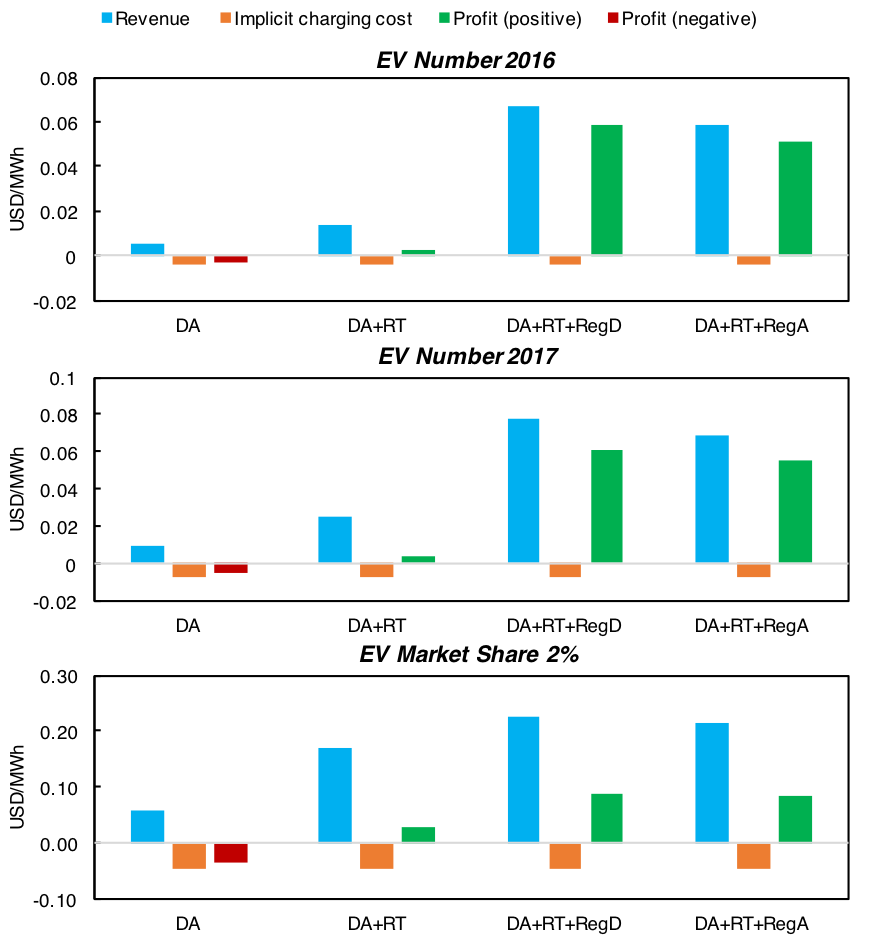
\includegraphics[width=0.9\linewidth]{Figures/PJM_EV_profit}
	\caption{Market size and profitability of EV2G in PJM Electricity markets}
	\label{fig:PJM_EV}
\end{figure}

Coupling frequency control markets increases the profits. However, we can see while the EV number increases from the scenario ``2017" to scenario ``2\% market share", the profitability drops significantly, as a result of exhaustion of liquidity, i.e. the frequency control markets will soon be saturated if it is indeed to implement all the EVs with EV2G and use them for frequency control services. Meanwhile, it shall be noticed that our analysis has overlooked some factors which could make the business less profitable as shown here. The main issue is that we use a determinate approach to simulate the frequency control signal and EV driving behaviors which eliminated the risks of failing to deliver the frequency control services as planned. Alipour \textit{et. al.}\cite{Alipour2017} made a study on EV2G for frequency control services with a stochastic approach. It was found in a case where a profit of 7980 USD was expected, the conditional value-at-risk was 5720 USD, indicating the risking nature of such a business. %In the outlook of this thesis, we proposed a stochastic method by using Markov chain to simulate the uncertain driving behavior of EVs and then the estimation of risk can be conducted. 
Nonetheless, while quantitative risk assessment against uncertainty is necessary for designing a specific project, it is beyond the focus of a study understanding the whole market value so is not included in our study. Besides, implementing EV2G for frequency control is not a mature technology due to its complexity\cite{Peng2017,Shafie-Khah2015,Bessa2014,Bessa2013}, which implies a high research and development cost.

It is also worthwhile to note that while the number of EVs in the scenario of ``2\% market share", the shares of  maximum achievable revenue by EV2G to the total market potential by generic ESS were between 8-27\% among different cases. Since the ``2\% market share" is close to the edge of power systems' affordable level for EV charging, this reveals EV2G will not be able fully cover the needs for flexibility by its own, even on a aggregated system level without considering the distributed manners. Other types of flexibility would still be necessary to complement the demands for flexibility in scenarios with high EV penetrations.

We further provide the profit for ``2\% market share" scenario in absolute values and values per EV, listed in Table \ref{tab:PJM-EV-profit}. These values should be of reference for market player to estimate the feasibility of business cases. For example, the maximum profit per EV is 126.3 which could indicate the proper incentive fees paid for end-users.

\begin{table}[h!]
	\footnotesize
	\centering
	\begin{tabular}{l r r r r}%L{2cm} R{2cm} R{2cm} R{2cm} R{3cm}}
		\hline
		& DA & DA+RT & DA+RT+RegD & DA+RT+RegA \\
		\hline
		\textit{in mUSD/yr}&    -28.0 	& 22.9& 	 66.4 &	 63.4  \\
		%\hline
		\textit{in USD/EV} &      -53.1 &	 43.5 	& 126.3 &	 120.5    \\ 
		\hline
	\end{tabular}
\caption{Profits of EV2G in PJM in the scenario of ``2\% market share"}\label{tab:PJM-EV-profit}
\end{table}
%and it was found to be more promising with the drastic of EVs as there are still much more growth space till the scenario of 2\% EV market share.

%However, with a 2\% EV market share, we saw a profit from business case while it incurred loss in Germany's DA+ID markets. 

%The drop of profitability is resulted from liquidity constraints. In fact, with a 2\% EV market share, there is a total of 1 week where the liquidity constraints is not fulfilled in order to deliver energy for EV charging. We discarded the revenue in that week which could be approximate 2\% of the actual total revenue. 

%This can be explained by the PJM's real-time market as a hub for all real-time settlements has much higher liquidity than the intra-day exchange in Germany.




%Similar studies are performed in PJM power markets.

%With these numbers of EV, no generation shortage was observed, expect for only one week in the scenario of 2\% EV market share. The results in that week were discarded, i.e. no operations and thus no revenues in that week. This accounts for approximately 2\% of the time in a year so the impact on final results shall be negligible.


%The incremental revenue by stacking RegD to DA+RT case was 462 USD/$(\text{a} \cdot \text{MW})$ in the scenario of ``EV Number 2016" while the additional revenue by stacking SCR to DA+ID in Germany was merely 206 USD/$(\text{a} \cdot \text{MW})$, which again reveals the favor of RegD toward flexibility resources. 

%Noticing that the whole RegD market potential for generic flexiblity resources is merely 513 USD/$(\text{a} \cdot \text{MW})$ as was shown previously by \ref{fig:pjm-ess}. This market could be easily exhausted by a small size of EV fleet. 

\subsubsection{EV2G profitability and market potential in DE}

Similar results are observed in Germany as shown in Figure \ref{fig:Germany_EV}


\begin{figure}[h!]
	\centering
	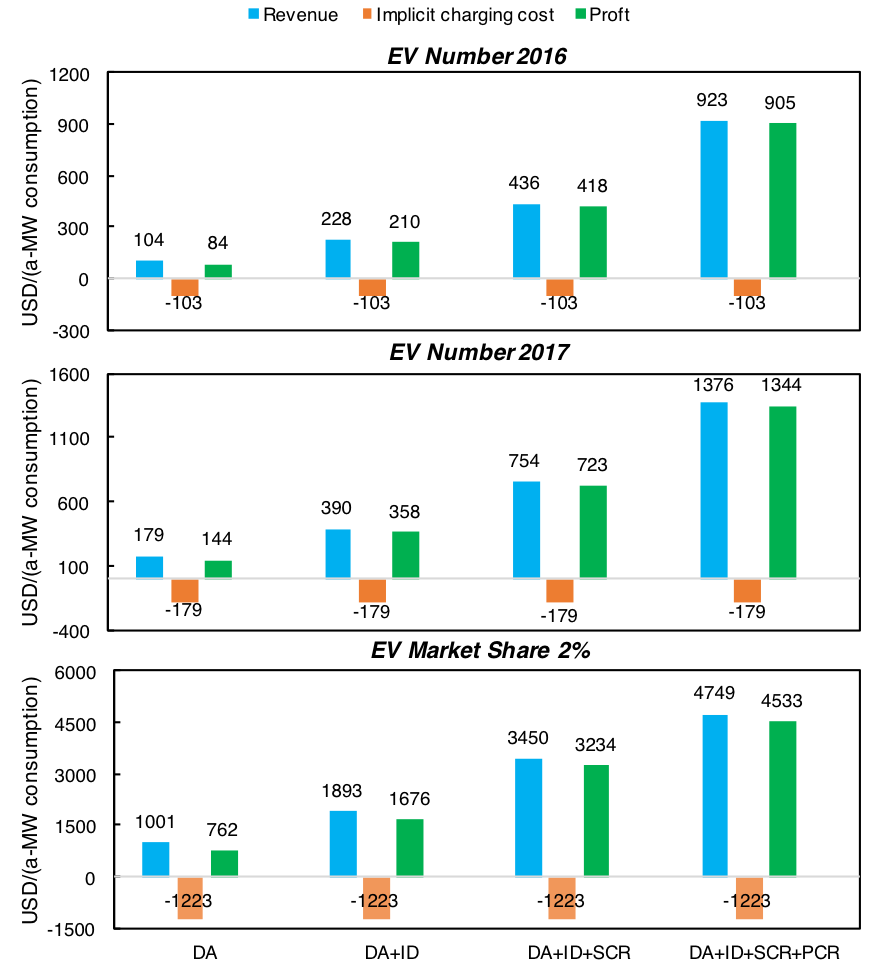
\includegraphics[width=0.95\linewidth]{Figures/Germany_EV_profit}
	\caption{Market size and profitability of EV2G in Germany electricity markets}
	\label{fig:Germany_EV}
\end{figure}

It was found that the arbitrage only in day-ahead market was not profitable at all, while arbitrage in both day-ahead and intra-day market was barely able to maintain a revenue-cost balance. The revenues captured from arbitrage was at most compensating the cost of EV charging. Profits would be possible if a business model where services providers could charge service fees from the end-users. Although the service fees can be much lower than the normal charging costs for the end-consumers, it would be still challenging in practice to implement such a business model because the charging cost become implicitly embedded when a EV was used for V2G services. In reality EV owners should be more likely to have the motivation to participate being paid with incentive fees. Overall, the low arbitrage values in Germany's energy market makes these business cases not appealing. 

We also provide the profits in the scenario of ``2\% market share" in mUSD/yr and USD/EV. It was found that profit per EV is close the values obtained in PJM.
%It is also worthwhile to note that while the number of EVs (0.9 million ) in the scenario of ``2\% Market Share" has reached the edge of the affordable level (1 million) for the grid, revenues are significantly smaller than the maximum potential revenues derived in the case studies of ESSs. The shares of maximum achievable revenue by EV2G to the total market potential by generic ESS were between 18-37\% among different cases. This reveals that constrained by the limitations discussed above, EV2G will not be able fully cover the needs for flexibility by its own, even on a aggregated system level without considering the distributed manners. Other types of flexibility would still be necessary to complement the demands for flexibility in scenarios with high EV penetrations.

\begin{table}[h!]
	\footnotesize
	\centering
	\begin{tabular}{l r r r r}%L{2cm} R{2cm} R{2cm} R{2cm} R{3cm}}
		\hline
		& DA & DA+ID & DA+ID+SCR & DA+ID+PCR+SCR \\
		\hline
		\textit{in mUSD/yr} &  -40.2& -15.1&	 94.2& 	 174.4\\
		%\hline
		\textit{in USD/EV} &  -44.7& 	 -16.8& 104.7&	 193.8\\ 
		\hline
	\end{tabular}
	\caption{Profits of EV2G in Germany in the scenario of ``2\% market share"}\label{tab:DE-EV-profit}
\end{table}


\subsubsection{EV2G profitability and market potential in NSW}

%Using the same methodology as in PJM, scenarios are established by taking the identical EV numbers per household, as is shown by Table \ref{tab:ev-number-scenario-nsw}. With these number of EV, no supply shortage was observed.  

%\begin{table}[h!]
%	\centering
%	\begin{tabular}{ l r r }
%		\hline
%		\textbf{Scenario} & \textbf{EV number total} & \textbf{EV number per household} \\
%		%\hline
%		\hline
%		EV number 2016 &  \num{4849} & \num{0.014} \\
%		EV number 2017 &  \num{8383} & \num{0.025} \\
%		2\% market share &  \num{58377} & \num{0.174} \\
%		\hline
%	\end{tabular}
%	\caption{The number of EV for each scenario in NSW}\label{tab:ev-number-scenario-nsw}
%\end{table}

\begin{figure}[h!]
	\centering
	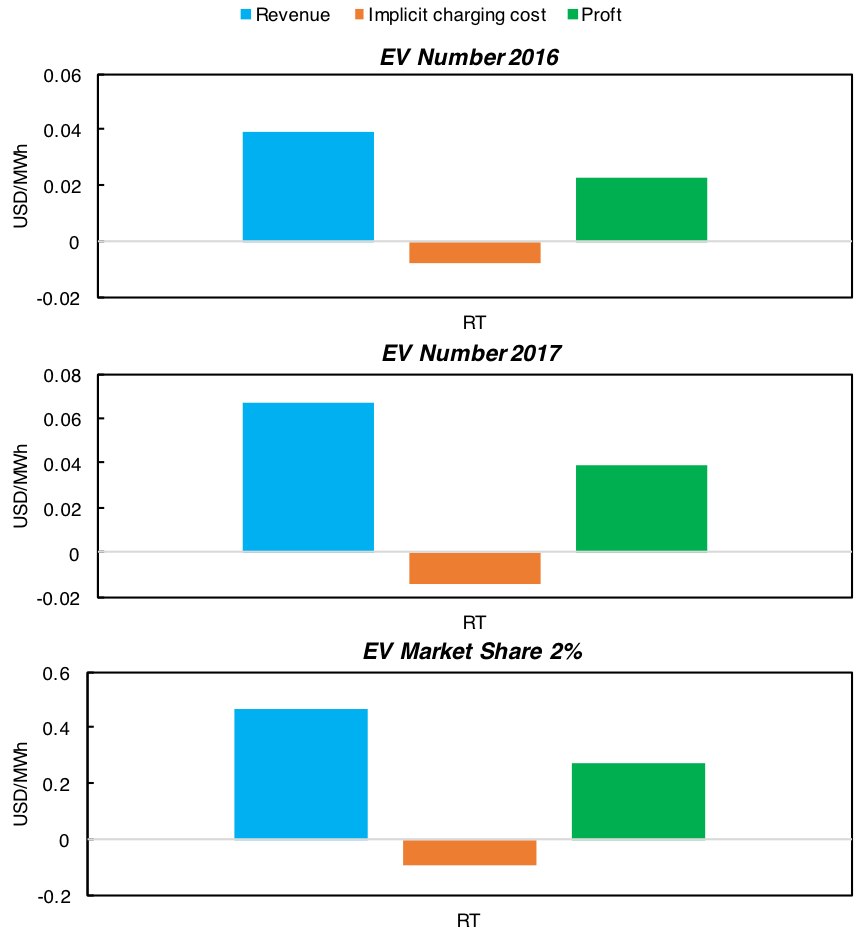
\includegraphics[width=0.8\linewidth]{Figures/NSW_EV_profit}
	\caption{Market size and profitability of EV2G in NSW Electricity markets}
	\label{fig:NSW_EV}
\end{figure}

Figure \ref{fig:NSW_EV} presents the results of three scenarios in NSW's real-time energy market. Similar to the situations in BESS cases, the market potential of arbitrage is higher than the other two geographies due to the price volatility as is cussed previously. The potential profit obtained in the scenario of ``EV Number 2016" was 0.02 USD/MWh, which was 66 and 9 times the numbers in corresponding cases in Germany and PJM respectively. It is even higher than profits from business cases where frequency control are involved in Germany. Since arbitrage using EV is much more feasible in technology, such a high arbitrage profitability shall provide more incentives for the market participates and makes the business appealing if the number of EV will indeed grow in line with our scenarios.

The profit in the scenario of ``2\% market share" is 19 mUSD/yr, or 325.6 USD/EV. The profit per EV is also much higher than in the other regimes, which makes it easier to acquire end-users' participation.


\subsection{Impact analysis of renewable penetration}
\label{sec:impact-market-condition}

As is mentioned several times in this thesis, understanding the impact of some key factors is crucially viable to plan future business on flexibility management, as the market may evolve rapidly. Among all the factors, we have selected the penetration of RES energy sources (RESs) as the most influencing factor and studied in this thesis. The rationale can be explained as the renewable penetration would change most radically compared to other factors and is viewed as the essential driver of growing needs for flexibility, which has been elaborated in Chapter \ref{ch:introduction}. 

Growing capacity of renewable generations will influence both wholesale energy and frequency control markets as we have seen from the literature; refer to Chapter \ref{ch:LitRev}. However, determining the requirement for frequency control reserve is an extremely sophisticate process of grid planning, which is rarely addressed by academic articles. Grid planner may initiated large-scale research project dealing with this problem. Referring to a study ordered by PJM and conducted by a research consortium led by GE Consulting\cite{GEEnergyConsulting2014}, an average of 1533 MW frequency regulation reserve would be required in a scenario where the 14\% RPS (Renewable Portfolio Standard by each state in PJM region) is to be met by 2026. This is about 2.2 times of the amount in 2016 (700MW). Assuming the price stays at the same level, one may multiply the ratio of 2.2 to the valuation results presented in preceding section, in order to make a rough estimation of the future. Nonetheless, the penetration of RES will not only influence the frequency control market physically but also institutionally where the design of market may be revised. Therefore, understanding quantitatively the impacts of RES on both volume and price in frequency control market are significantly beyond the scope of this study. 

In this thesis, we would only focus on the wholesale energy market. Day-head markets in both Germany and PJM are taken for case studies.

In order to simulate price scenarios with different level of renewable generation, we adopted a simplified method by multiplying the time-series data of actual renewable generation in 2016 by a certain ratio. No simulations with wealth data were involved. 

In Germany, the installed capacity of solar and wind has already accounted for a significant share, i.e. \num{83.85} GW as 41.7\% of the total generation capacity. Therefore, we made conservative scenarios where the assumed capacity of wind and solar are 85\% to 115\% of present level with a step length of 5\% of the existing capacity, equal to 4.19 GW per step. 

%\num{105870 } GWh 2016 in Germany, including both wind and solar generations. Therefore, a change of 5\% in renewable generation can be deemed as equivalent to 4.19 GW or \num{8.29} GWh. 


For PJM, the installed capacity of wind and solar was merely 6533 MW in 2016, which is 3.7\% of the total capacity. The 14\% RPS, as is mentioned above, requires PJM to install a total of \num{40190} MW solar and wind generations by 2026. Compared to the number in 2016, this indicates a compound annual growth rate (CAGR) of 20\%. Therefore, we created additional scenarios beyond the ones that are consistent with German cases (85-115\%) as 5-year forecasts the 20\% CAGR.

\subsubsection{Model setup and validation}
In order to analyze the future trend of market value by understanding potential impacts of certain key factors, the market simulation module was designed as is introduced in Section \ref{sec:market-simulation}. In this section, we would demonstrate the setup and validation of the module  based on day-ahead market and generation data in Germany in 2016.

First of all, the data of Germany day-ahead price and volume were collected and shown as Figure \ref{fig:merit-orignal}.

\begin{figure}[h!]
	\centering
	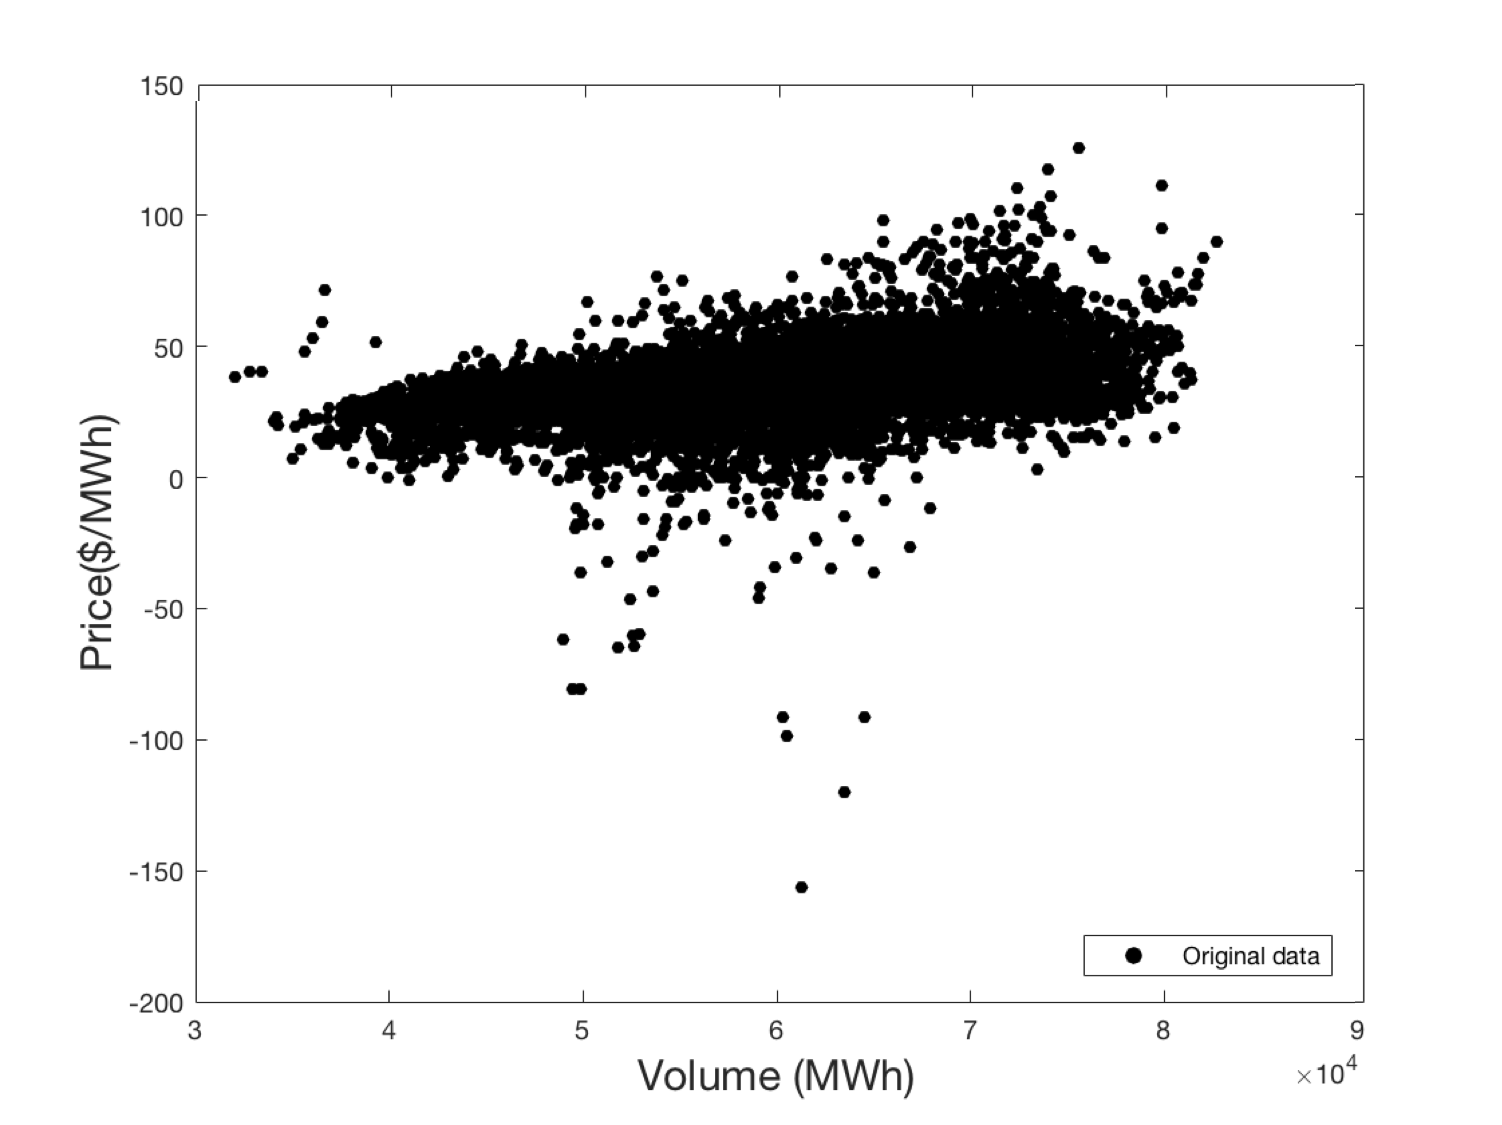
\includegraphics[width=0.95\linewidth]{Figures/Merit-order-original}
	\caption{Germany day-ahead price-volume data in 2016}
	\label{fig:merit-orignal}
\end{figure}

The pattern of merit-order effect is not clearly recognizable from the original data mainly due to the disturbs of variable renewable generation which has raised significantly in past years. This prevents us from directly applying merit-order models developed by previous studies\cite{He2013}\cite{Grunewald2012a}. Therefore, we applied the algorithm described in Section \ref{sec:market-simulation} which take into account the renewable generation and bounded flexibility of conventional generations. Figure \ref{fig:merit-transformed} shows the transformed pattern of data where a clearer merit-effect is identifiable. Figure \ref{fig:merit-classified} projects the classification to the original data distribution and it can be seen that the algorithm has successfully separated the data points where the price was driven to be higher or lower than average level due to the uplift effects introduced in \ref{sec:market-simulation}. 

\begin{figure}[h!]
	\centering
	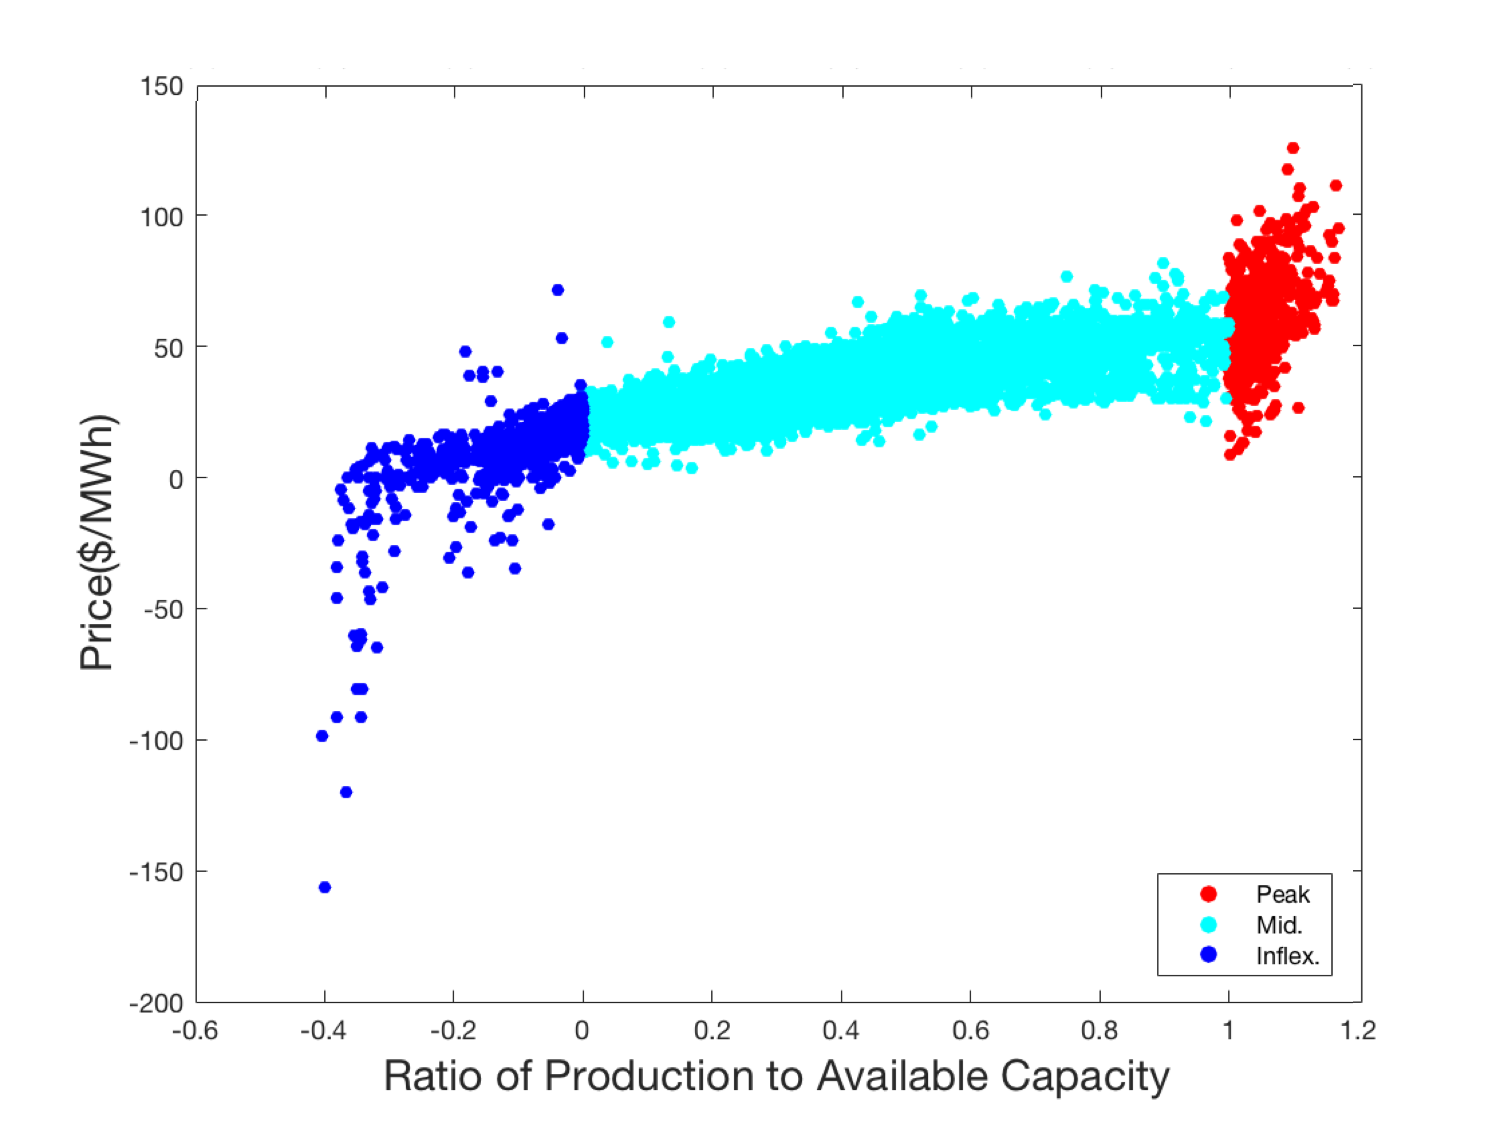
\includegraphics[width=0.95\linewidth]{Figures/Merit-order-transformed}
	\caption{Transformed pattern of Germany day-ahead price-volume data in 2016}
	\label{fig:merit-transformed}
\end{figure}
\begin{figure}[h!]
	\centering
	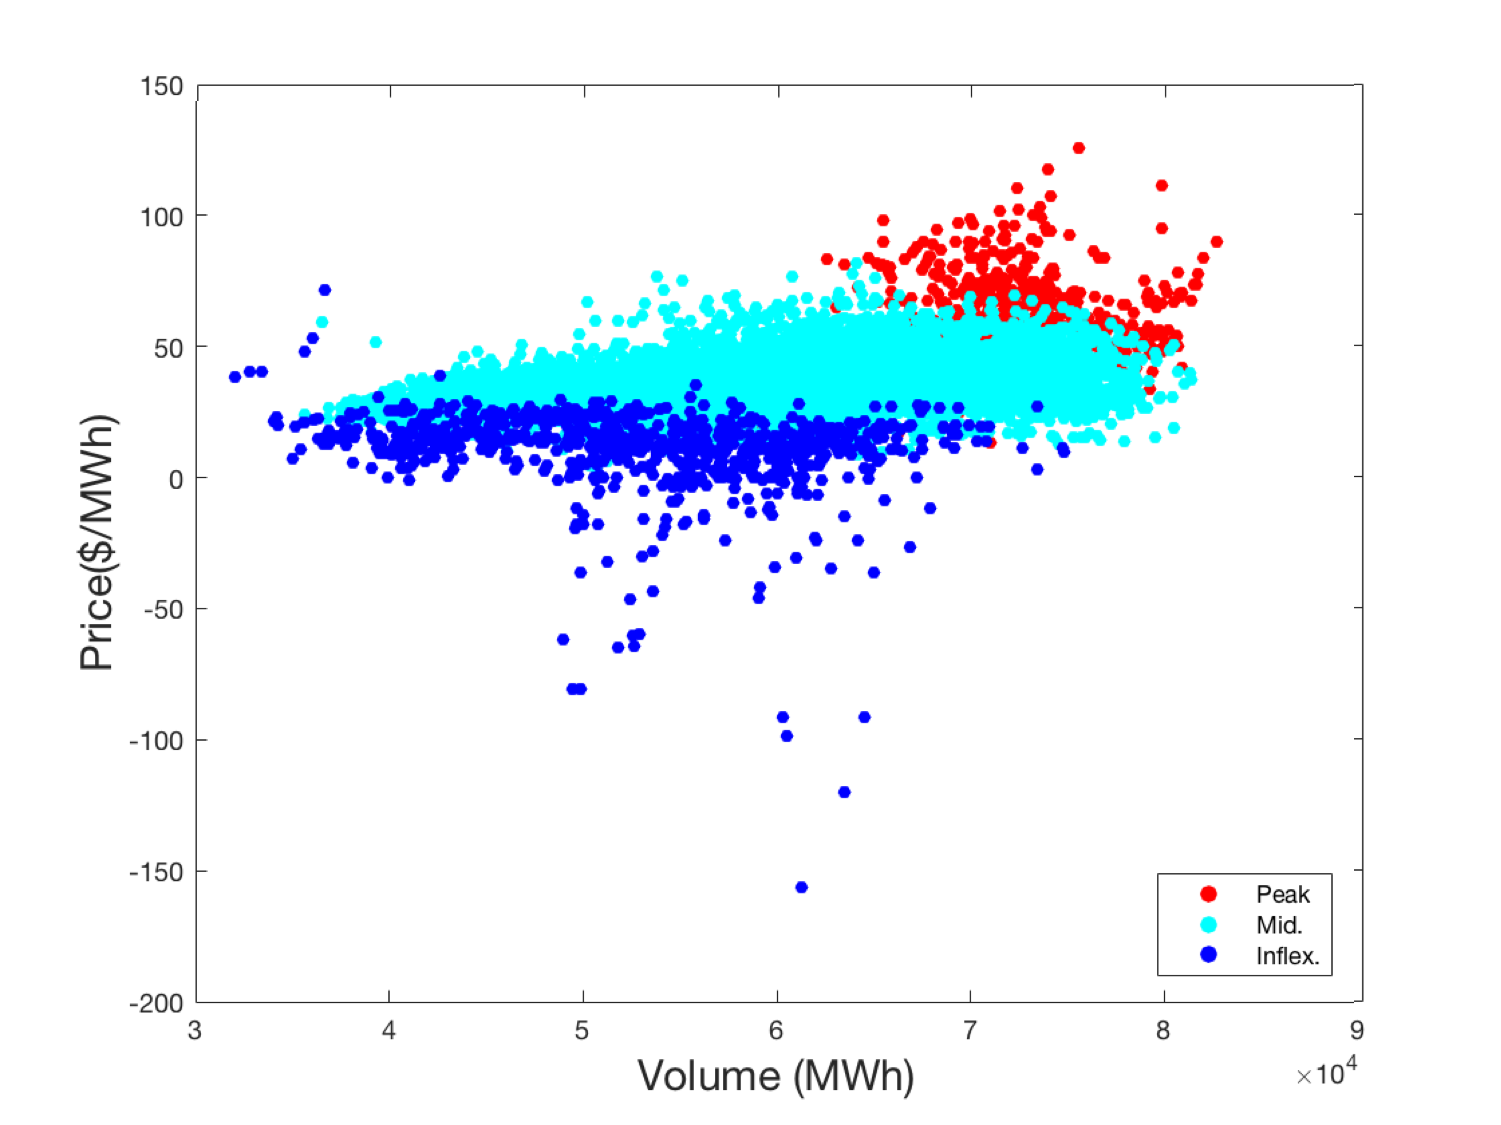
\includegraphics[width=0.95\linewidth]{Figures/Merit-order-classified}
	\caption{Classification of Germany day-ahead price-volume data in 2016}
	\label{fig:merit-classified}
\end{figure}

Thereafter, we fitted the transformed data pattern with the piece-wise function defined by \eqref{eq:merit-order-model}. The estimated parameters are listed in Table \ref{tab:merit}. It shall be noticed there are price limits applied in EPEX day-ahead market\cite{EPEX_price_limit} which is between -500 to 3000 EUR/MWh, equal to -600 to 3600 USD/MWh using the specified currency exchange rate. The fitted merit-order curve is illustrated by Figure \ref{fig:merit-fitted} and distribution of errors between the fitted price and actual price is shown by Figure \ref{fig:merit-error}.

\begin{table}[h!]
	\centering
	\begin{tabular}{l  r r r}
		\hline
		\multirow{2}{*}{\textbf{Class}} & \multicolumn{3}{c}{\textbf{Parameters}}\\
		& $a$ & $b$ & $c$\\
		\hline
		Inflex. & 17.05 & 1.49 & 12.35 \\
		\multirow{3}{*}{Mid.} & 48.66 & 16.40 & \\
		\multirow{3}{*}{} & 38.04 & 20.12 & \\
		\multirow{3}{*}{} & 16.37 & 34.20 & \\
		Peak & 1.95 & 491.46 & 0.69 \\
		\hline
	\end{tabular}
	\caption{Parameters of the merit-order model in Germany}\label{tab:merit}
\end{table}

\begin{figure}[h!]
	\centering
	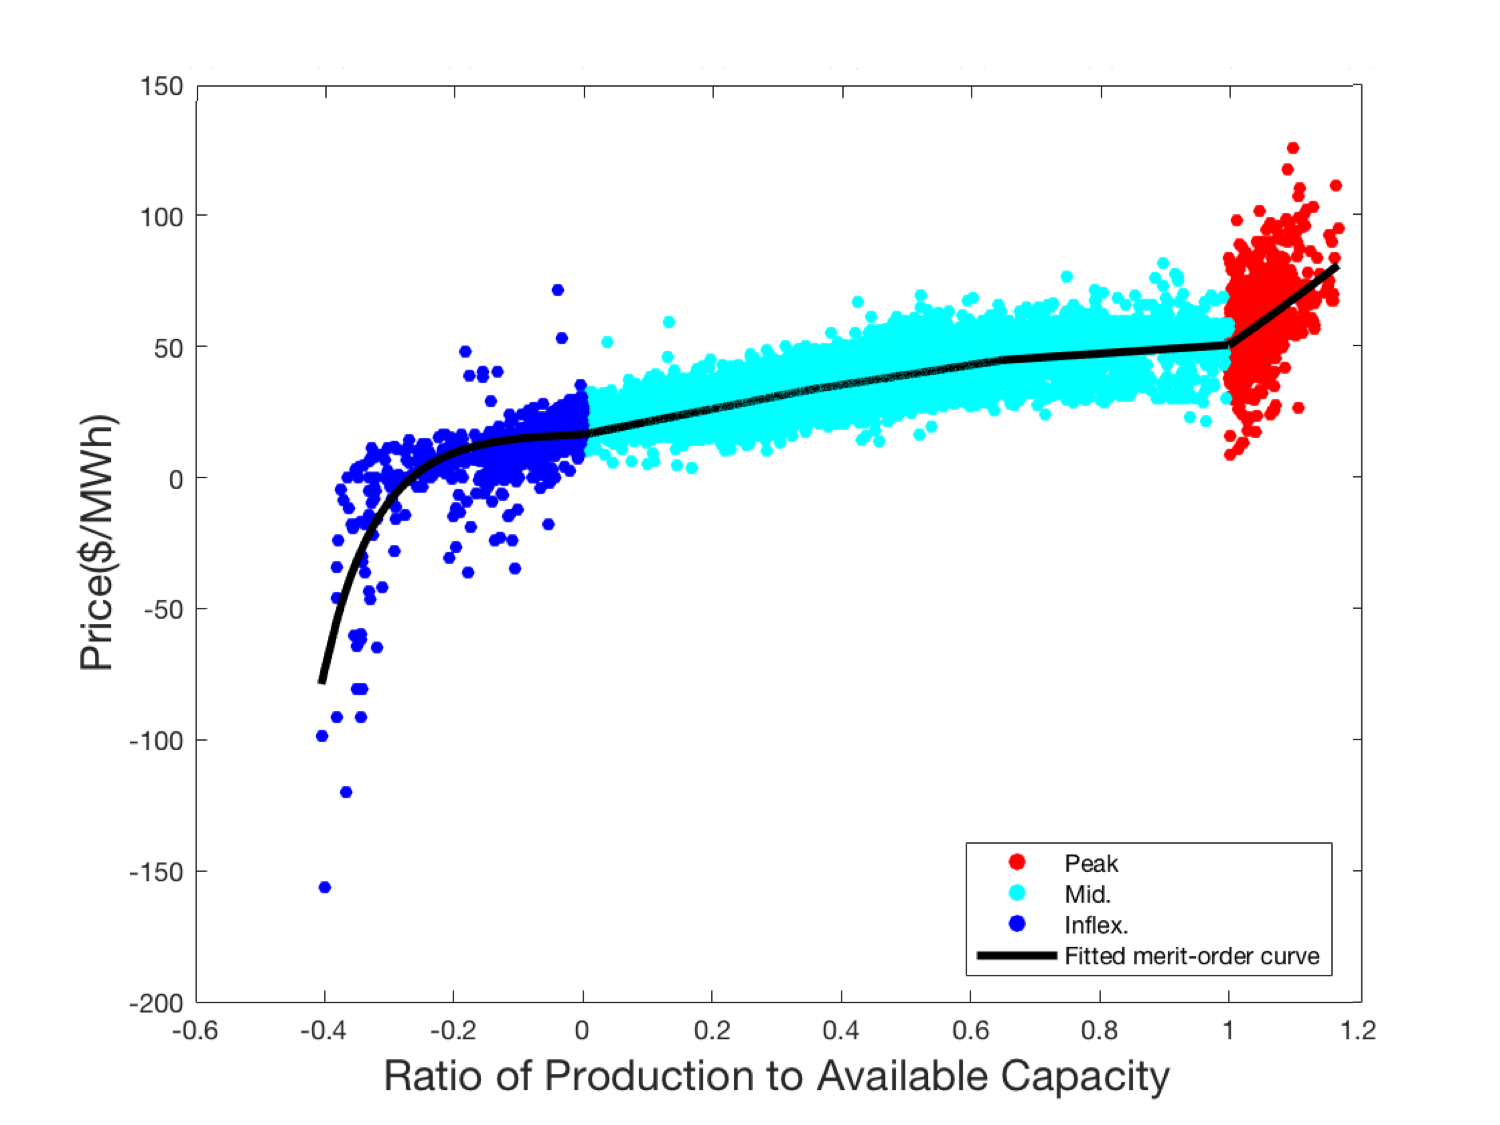
\includegraphics[width=0.95\linewidth]{Figures/Merit-order-fitted}
	\caption{Fitted merit-order curve with Germany day-ahead price-volume data in 2016}
	\label{fig:merit-fitted}
\end{figure}

\begin{figure}[h!]
	\centering
	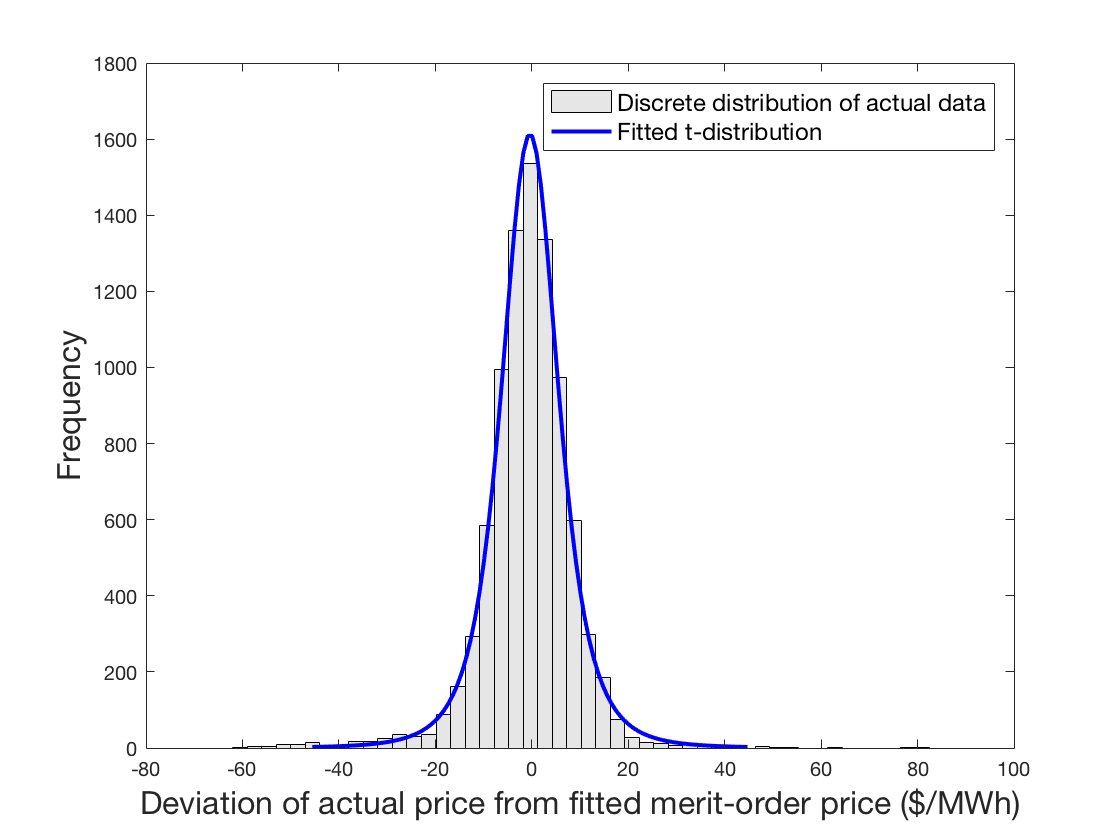
\includegraphics[width=0.9\linewidth]{Figures/4_Error-distribution}
	\caption{Distribution of errors between fitted merit-order price and actual price}
	\label{fig:merit-error}
\end{figure}

We simulated the day-ahead price using this merit-order model and compared to the actual market data. It can seen from Figure \ref{fig:merit-fitted}-\ref{fig:merit-error} that while the fitted merit-order price shows a good fitness to the actual price in terms of general trend, the stochastic movements of the price are eliminated. Merely with the merit-order model, a smoothed curve of price time-series would be generated where the drastic jumps of price cannot be captured, as is demonstrated by Figure \ref{fig:price-example}.

\begin{figure}[h!]
	\centering
	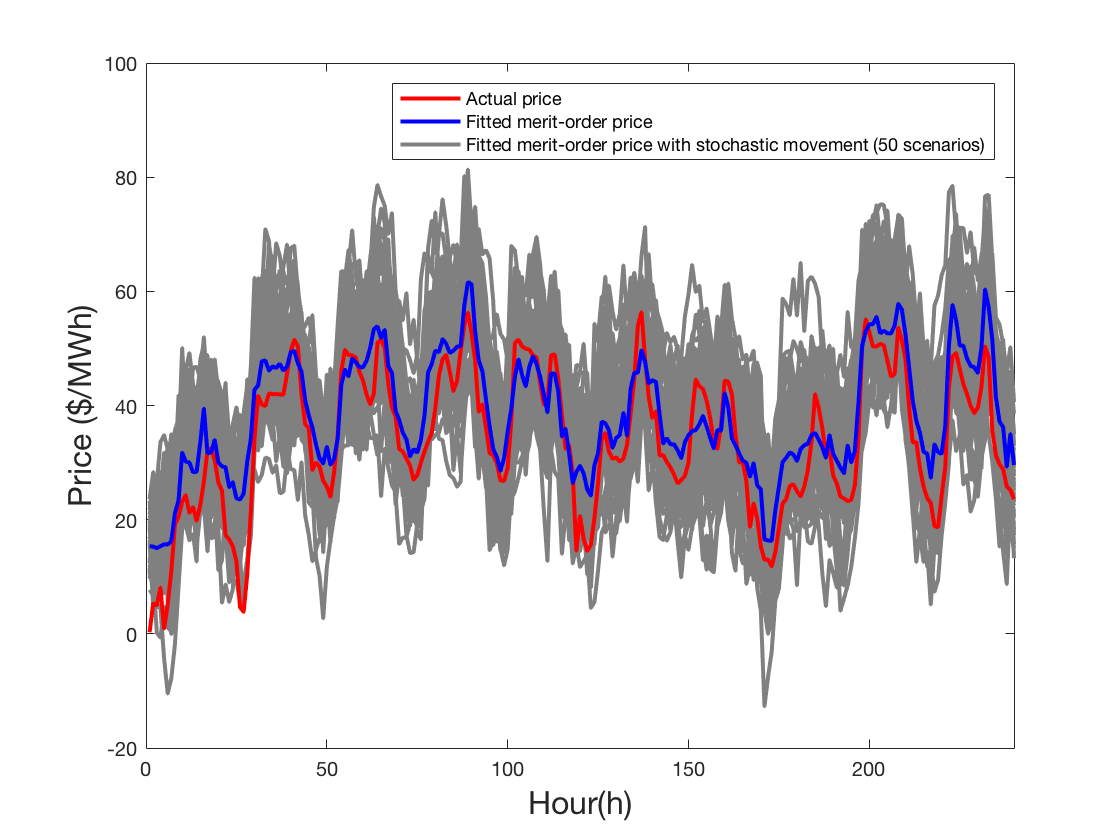
\includegraphics[width=0.95\linewidth]{Figures/5_Example-simulated_price}
	\caption{Generated price scenarios}
	\label{fig:price-example}
\end{figure}

Unlike studies on valuation of a conventional generation resources where such a merit-order model may suffice, the elimination of stochastic price movement would reduce the value of arbitrage greatly as is shown by Figure \ref{fig:model-validation}. This shall be understood intuitively as arbitrage activities pick the price differences among different trading slots and less volatile price movements would certainly affect the value creation of arbitrage.

\begin{figure}[h!]
	\centering
	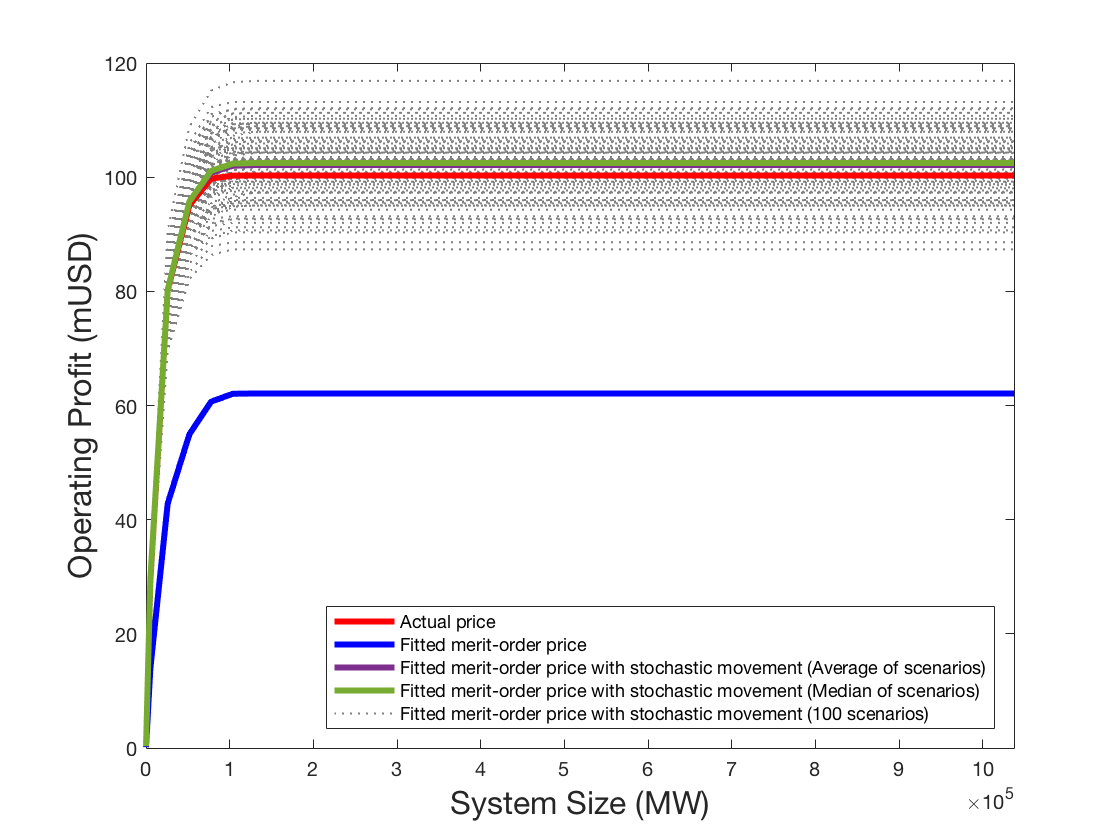
\includegraphics[width=0.95\linewidth]{Figures/6_Model_Validation}
	\caption{The revenue with different price scenarios for model validation in Germany}
	\label{fig:model-validation}
\end{figure}

\begin{table}[h!]
	\centering
	\begin{tabular}{r r}
		\hline
		\multicolumn{2}{c}{SARMA parameters}\\
		\hline
		$\omega_1 = 1.811$ & $\theta_1 = -1.063$ \\
		$\omega_2 = -0.813$ & $\theta_{24} =0.692$ \\
		$\omega_{24} = 0.090$ & $\theta_{168} = -0.600$ \\
		$\omega_{168} = 0.692$ & \\
		\hline
	\end{tabular}
	\caption{Parameters of the stochastic price movement of SARMA models in Germany}\label{tab:SARMA}
\end{table}

Therefore, a seasonal auto-regressed moving-average (SARMA) model as is described in \ref{sec:market-simulation} is applied to simulate the stochastic components of the price. The estimated parameters of the SARMA model based on the error signal characterized by\ref{fig:merit-error} is listed in Table \ref{tab:SARMA}. Thereafter, we conducted Monte-Carlo simulations and generated a number of scenarios of the stochastic parts of price which are then added to the determinate trends calculated by the merit-order model. The final simulated price scenarios are illustrated by the grey lines in Figure \ref{fig:price-example}. Using these generated price profiles, we calculated the revenue for 100 scenarios and compare the average and median value to the result obtained with actual price signal, which shew perfect fitness in Figure \ref{fig:model-validation}. There are no significant differences between the average and median value observed, but for robustness and avoiding effects of outliers, we would use the median value as the simulated result for experiments in proceeding sections.

We applied the same procedure to develop the model for PJM. It was noticed that the situation when the residual load is in the range of inflexible generation is rarely observed in PJM, which can be explained by the relative low installed capacity of renewable generations. Therefore, we migrated part of the merit-order model for inflexible generation based on Germany's data here, which shall however have insignificant effects because the lowest price is bounded at 0. Negative pricing is not explicitly an issue in PJM's market so far although PJM is fully aware of this issue but waiting for FERC's initiative to address the potential negative price formation\cite{PJM_price_limit_1}. Without unambiguous rules, we would not allow negative prices in our modeling. The highest price, on the other hand in PJM is capped at 1000 USD/MWh\cite{PJM_price_limit}. 

The parameters for the merit-order model in PJM are listed in Table \ref{tab:merit_pjm}. The SARMA parameters are presented in Table \ref{tab:SARMA_PJM}.

\begin{table}[h!]
	\centering
	\begin{tabular}{l  r r r}
		\hline
		\multirow{2}{*}{\textbf{Class}} & \multicolumn{3}{c}{\textbf{Parameters}}\\
		& $a$ & $b$ & $c$\\
		\hline
		Inflex. & 17.05 & 1.49 & 12.35 \\
		\multirow{3}{*}{Mid.} & 23.50 & 16.40 & \\
		\multirow{3}{*}{} & 32.02 & 13.41 & \\
		\multirow{3}{*}{} & 3.58 & 31.90 & \\
		Peak & 10.70 & 501.35 & 5.32 \\
		\hline
	\end{tabular}
	\caption{Parameters of the merit-order model in PJM}\label{tab:merit_pjm}
\end{table}

\begin{table}[h!]
	\centering
	\begin{tabular}{r r}
		\hline
		\multicolumn{2}{c}{SARMA parameters}\\
		\hline
		$\omega_1 = 0.690$ & $\theta_1 = 0.107$ \\
		$\omega_2 = 0.125$ & $\theta_{24} =-0.003$ \\
		$\omega_{24} = 0.298$ & $\theta_{168} = -0.399$ \\
		$\omega_{168} = 0.560$ & \\
		\hline
	\end{tabular}
	\caption{Parameters of the stochastic price movement of SARMA models in PJM}\label{tab:SARMA_PJM}
\end{table}


\subsubsection{Renewable penetration in Germany}


\begin{figure}[h!]
	\centering
	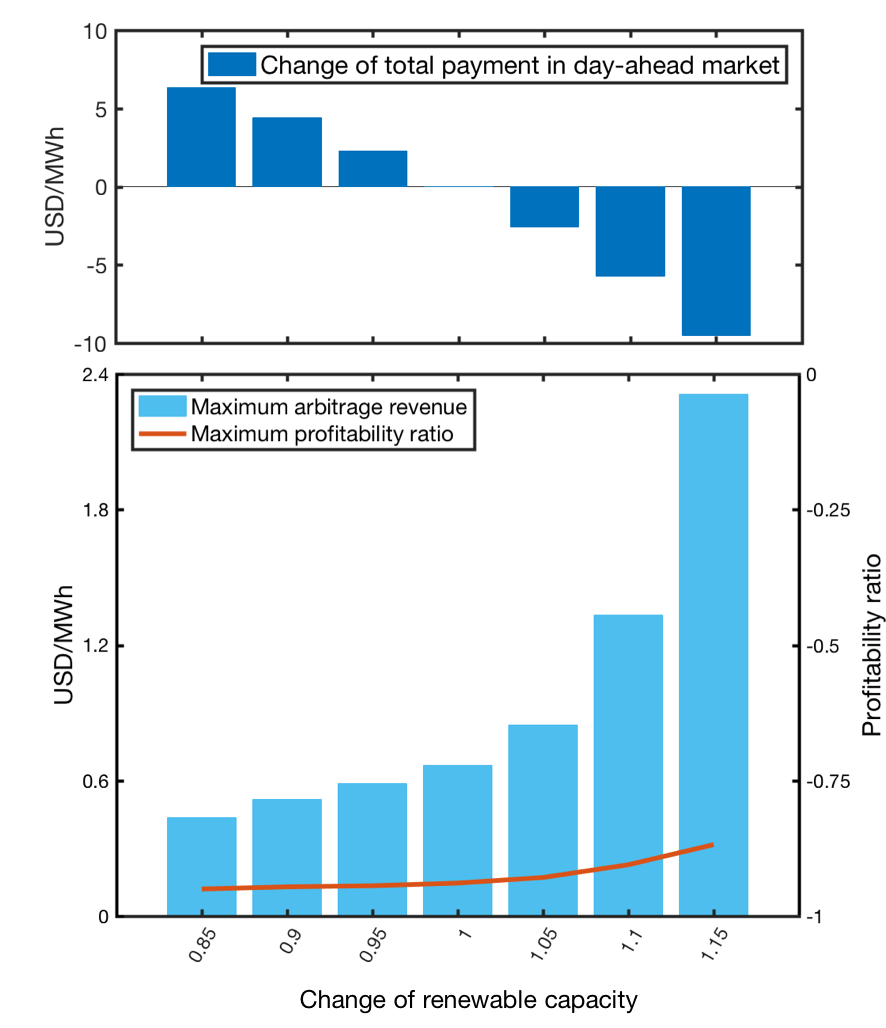
\includegraphics[width=0.95\linewidth]{Figures/RenewablePenetration_Germany}
	\caption{Impacts of renewable generations on revenue and profitability of arbitrage using flexibility as well as on total amount of transations in day-ahead market in Germany}
	\label{fig:renew_germany}
\end{figure}

The results are illustrated in Figure \ref{fig:renew_germany}. We can see while the revenue potential of arbitrage using flexibility grew insignificantly with renewable capacity growing from 85\% to the present level, it would accelerate rapidly afterwards. The potential revenue would almost double its value with 10\% additional renewable generation and triple with 15\% renewable growth. This indicates the day-ahead market in Germany is at a inflection point where the volatility will increase drastically with more renewable making it more favorable for arbitrage. Quantitatively, it was found when renewable capacity grew from 85\% to the present level, the addition of each 5\% growth would lead to a increase of 12-23\% on the
the standard deviation of day-ahead price. In contrast, the rises of volatility would be 74-225\% for each additional 5\% growth of renewable growth from present level to 115\%.

However, it is known that the renewable penetration will not only increase the price volatility but also lower the average level of price via the so-called merit-order effect. In our study, the merit-order effect was found to be 0.75 - 1.12 USD/MWh per additional GW of renewable generation, which accords with the number found by previous research where the merit-order effect was accounted to be 0.8-2.3 EUR/MWh  per additional GW in Germany by statistic studying on the real data between 2008 to 2012. 

Without any interventions, this effect would soon make the price unacceptably low to generators. In the scenario with 15\% more renewable the average price in day-ahead energy market will reduce by 9.5 USD/MWh which would be over one third of the revenues received by generators as a whole. The growth of arbitrage revenue would be one order of magnitude smaller than the reduction of overall amount of payment to generators. It was certain that players will take actions against this trend. The policy supports on RES may also be gradually abated as what have already been noticed from the real world and introduced in Section \ref{sec:qualitative-analysis}. 

Market players with conventional generations that are suffering the pressure of decreasing price due to RES may embrace flexibility in order to mitigate the conflicts of RES and inflexible generations or even enhance their market power to strategically maintain the price level as is studied in \cite{Schill2011}. The effects of arbitrage using flexibility on wholesale energy market would be briefly discussed in Section \ref{sec:sensitivity} on a schematic level.

Nevertheless, BESS might not be the right choice to achieve these goals. As the profitability ratios of the pre-defined BESS in our study were still deeply negative and raised insignificantly to be optimally -87\% from nowadays's level of -94\%.

\subsubsection{Renewable penetration in PJM}

Similar work was conducted in PJM's day-ahead market. Results are shown by Figure \ref{fig:renew_pjm}. With trivial addition of renewable generations from 85-115\%, the potential arbitrage revenue would increase slightly by about 0.7-1\% for each 5\% increment. However, further growth of RES will lead to a decreasing trend of arbitrage potential. This could be explained because of the non-negative price. Without compensation from negative prices, the arbitrage value dropped along with the shrink of average electricity price due to merit-order effects. The merit-order effect here was found to be 1.05 - 1.13 USD/MWh per additional GW of renewable capacity.

\begin{figure}[h!]
	\centering
	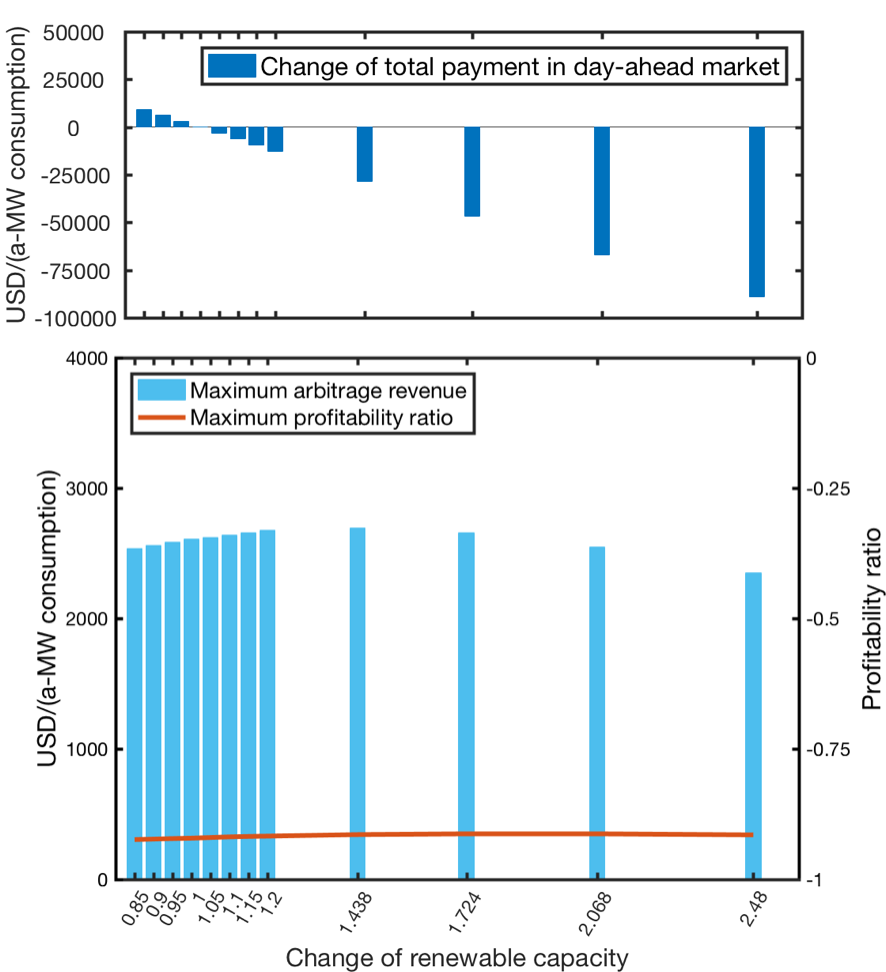
\includegraphics[width=0.95\linewidth]{Figures/RenewablePenetration_PJM}
	\caption{Impacts of renewable generations on revenue and profitability of arbitrage using flexibility as well as on total amount of transations in day-ahead market in PJM}
	\label{fig:renew_pjm}
\end{figure}

PJM reported that it had received negative offers from wind generation enabled by the federal wind production tax credit (PTC)\cite{PJM_price_limit_1}. However, without a clear framework of negative price formation, predictive studies would hardly be robust. 

\subsection{Sensitivity analysis}
\label{sec:sensitivity}
Throughout the whole study, the most crucial assumption made is the perfect predictability. Elaborated in the literature, this assumption is common pragmatic ways in similar studies to indicate a idealistic value as upper bound. Nonetheless, it is necessary to study how reliable the results are based on these assumptions. 
%Throughout the whole study, there are two crucial assumption made, i.e. the perfect predictability assumption and fixed price assumption. Elaborated in the literature, this two assumptions are common pragmatic ways in similar studies to indicate a idealistic value as upper bound. Nonetheless, it is necessary to study how reliable the results are based on these assumptions. Besides, the sensitivities of other parameters that were determined based on assumptions are also tested in this section.
%\subsubsection{Limited predictability}

In reality, players have a set of methods to forecast the price in short run, some of which are quite efficient and accurate \cite{Weron2014} so close to the perfect forecast assumption. However, while valuing the total market, we shall view the market as whole where players' ability of predicting vary significantly. Therefore, here we would calculate the maximum deviations from our previous estimations in a worst case scenario, i.e. deriving the lower bounds, where players' forecasting ability is poor. This worst forecast method is defined as ``back-cast" as is explained in Section \ref{sec:perfect-forecast}, via which market participates directly take the historical price to foresee the future price. This is the simplest way of forecasting the price and is feasible for all players without the needs for any modeling abilities, so shall indeed represent the lowest possible values.

We tested two scenarios where the price is lagged by 1 day and 1 week respectively, i.e. taking the day-ahead and week-ahead price as the predicted price. The BESS with ``small size" and EV2G with ``number in 2016" are picked for carrying out the sensitivity analysis. 

The results are summarized in Table \ref{tab:sensitivity-predict-germany} to \ref{tab:sensitivity-predict-nsw}.

\begin{table}[h!]
	\centering
	\begin{tabular}{L{3.6cm} R{2cm} R{2cm} R{2cm} R{2cm}}
		\hline
		\textbf{Case} & \multicolumn{2}{c}{\textbf{Backcast - 1 week}} & \multicolumn{2}{c}{\textbf{Backcast - 1 day}} \\
		& R\footnote{Revenue: difference in percentage }& PR\footnote{Profitability Ratio: difference in percentage point}& R$^a$ & PR$^b$ \\
		\hline
		\multicolumn{5}{l}{\textbf{BESS} }\\
		DA & -50.6\%& -2.3\% & -48.9\%& -2.1\% \\
		ID & -50.0\%& - 3.2\%&-52.5\%  & -4.1\%\\
		BE & -133.1\%& - 131.8\%&-101.3\%  & -112.2\%\\
		PCR & -0.0\%& - 0.0\%&N.A.\footnote{Primary and secondary control markets are organized by weekly auctions} & N.A.$^c$\\
		SCR & -10.3\%& - 0.6\%& N.A.$^c$ & N.A.$^c$ \\
		DA+ID & -52.3\%& - 4.1\%& -52.1\% & -4.7\% \\
		DA+ID+SCR & -35.9\%& - 0.9\%& -38.6\% & -1.3\% \\
		DA+ID+PCR+SCR & -33.3\%& - 0.0\%& -33.0\% & -0.1\% \\
		\hline
		\multicolumn{5}{l}{\textbf{EV2G} }\\
		DA & -36.1\%& -1.2\% & -58.6\% &-1.8\% \\
		DA+ID & -41.5\%& -2.3\% & -59.0\% &-3.0\% \\
		DA+ID+SCR & -22.3\%& -1.1\% & -30.4\% &-1.6\% \\
		DA+ID+PCR+SCR & -11.6\%& -1.1\% & -22.0\% &-1.5\% \\
		\hline
	\end{tabular}
	\caption{Summary of sensitivity analysis on predictability in DE}\label{tab:sensitivity-predict-germany}
\end{table}

We first focus on the DE case since the it is of our particular interest in delivering balancing energy as the only profitable use-case in Germany but we doubted the feasibility as mentioned several time in previous sections. In Table \ref{tab:sensitivity-predict-germany}, the results for providing balancing energy indeed drops considerably, which verified our previous analysis that this market is not practically feasible for market players due to the volatility and unpredictability of balancing energy price, reBAP. The revenue decreases by over 100\%, which means without good forecast, using flexibility solutions may lead to more imbalance charges rather than avoid. 

Besides, we can see the cases involving arbitrage is more sensitive than cases with frequency control services. This implies that predicting price precisely for selling frequency control reserves is not as a critical issue as for arbitrage.

Finally, it was found while back-cast for 1 day had sightly better performance than back-cast for 1 week for BESS, the situation reversed for EV2G. This can be explained because EV driving behaviors embedded in our model also have a weekly pattern, as was shown in preceding section. It is necessary to matching EV driving profiles well with the price profiles.

\begin{table}[h!]
	\centering
	\begin{tabular}{L{3.6cm} R{2cm} R{2cm} R{2cm} R{2cm}}
		\hline
		\textbf{Case} & \multicolumn{2}{c}{\textbf{Backcast - 1 week}} & \multicolumn{2}{c}{\textbf{Backcast - 1 day}} \\
		& R\footnote{Revenue: difference in percentage }& PR\footnote{Profitability Ratio: difference in percentage point}& R$^a$ & PR$^b$ \\
		\hline
		\multicolumn{5}{l}{\textbf{BESS} }\\
		DA & -35.5\%& -1.9\% & -17.9\%& -1.1\% \\
		RegD & -4.4\%& -6.4\%&-4.4\%  & -5.1\%\\
		RegA & -33.3\%& -22.4\%&-26.7\%  & -19.3\%\\
		DA+RT & -51.6\%& - 7.2\%&  -39.5\%& -6.1\% \\
		DA+RT+RegD & -47.8\%& -5.4\%& - 36.7\%& -4.5\%\\
		DA+RT+RegA & -48.6\%& - 12.9\%& -37.2\% & -11.2\% \\
		DA+RT+RegD+RegA & -48.4\%& - 10.3\%& -34.7\% & -8.7\% \\
		\hline
		\multicolumn{5}{l}{\textbf{EV2G} }\\
		DA & -32.9\%& -0.9\% & -18.3\% &-0.6\% \\
		DA+RT & -50.3\%& -3.2\% & -43.8\% &-1.0\% \\
		DA+RT+RegD & -39.5\%& -2.5\% & -34.8\% &-2.3\% \\
		DA+RT+RegA & -41.9\%& -4.1\% & -36.4\% &-3.5\% \\
		DA+RT+RegD+RegA& -34.4\%& -4.1\% & -29.9\% &-3.5\% \\
		\hline
	\end{tabular}
	\caption{Summary of sensitivity analysis on predictability in PJM}\label{tab:sensitivity-predict-pjm}
\end{table}

Compared to results in Germany, the sensitivity of predictability shows a similar pattern. The revenue reduction is less significant in PJM's day-ahead market compared to Germany, implying a more stable price profile.  This can be explained that a power pool with capacity obligation can maximize the participation of all resources and suppress virtual transactions, thereby leading to a robuster price formation than a power exchange. Revenue potential from RegD altered sightly while the value from RegA significantly dropped. This is because in the original plans players were assigned with perfect predictability of frequency control signal as well so that they were able to better tackle the non-energy-neutral signal.  In reality, frequency control signals are impossible to forecast. Therefore, the merit of energy-neutral signal is again demonstrated. However, it shall be emphasized again that implementing energy-neutral signals is a complex and challenging task. A energy-neutral signal might be most beneficial to the system, since it might move to the same direction as the error in order to maintain energy neutrality. This is the rationale why PJM re-engineered the RegD to be conditional energy neutral. 

\begin{table}[h!]
	\centering
	\begin{tabular}{L{2.5cm} R{2cm} R{2cm} R{2cm} R{2cm}}
		\hline
		\textbf{Case} & \multicolumn{2}{c}{\textbf{Backcast - 1 week}} & \multicolumn{2}{c}{\textbf{Backcast - 1 day}} \\
		& MR\footnote{Max. Revenue: difference in percentage }& MPR\footnote{Max. Profitability Ratio: difference in percentage point}& MR$^a$ & MPR$^b$ \\
		\hline
		\multicolumn{5}{l}{\textbf{BESS} }\\
		RT & -58.8\%& -16.6\% & -47.6\%& -14.7\% \\
		\hline
		\multicolumn{5}{l}{\textbf{EV2G} }\\
		RT & -56.4\%& -13.8\% & -51.3\% &-12.7\% \\
		\hline
	\end{tabular}
	\caption{Summary of sensitivity analysis on predictability in NSW}\label{tab:sensitivity-predict-nsw}
\end{table}

In NSW, although we have pointed out the higher volatility in its real-time markets leads to a higher potential of arbitrage compared to markets in Germany and PJM, it also demands higher precision of price forecasting. The revenue and profitability dropped more sensitively than arbitrage cases in the other two geographies.

%\subsubsection{Responsive price}
%While the amount of flexibility reaches a significant level, their trading behaviors will certainly disturb the market and affect the price. Especially in the case of arbitrage where the price volatility is being utilized for value creation, the actual revenue would be more sensitively depending on the responsive price effect. Regarding frequency control market, the revenue relies on the average price level rather than the price volatility and the distinct price formation mechanism such as the pay-as-bid mode in German markets shall suppress significant disturbances of new players on market price. 

%Therefore, we studied the effect only on wholesale energy markets here. It shall be firstly pointed out, with a responsive price, there are still two distinct scenarios exist, i.e. price taker and price marker. In the price taker scenario, although the players' actions will affect the price formation, the market is highly competitive so each player has negligible market power. In contrast, price maker may exist in some markets where the competitions are sufficient and few players can strategically exert its market power to distort the market price. Among these two cases, it is clear that the price taker scenario would indicate a lower bound while price makers are more likely to receive higher payments or better fulfill their strategic goals. Therefore, in this section, we take the worst case scenario where players have no market power. It shall be noticed that in this scenario, their price forecast is not imperfect since the price formation takes place after their decisions are made. 

%The results for the day-ahead market in Germany as an illustrating example is shown by Table

%\textit{(To be continued)}
%\subsubsection{Sensitivity analysis of other parameters}

%\section{Summary of case studies}

\subsection{Summary of quantitative studies}

Recalling our initial research questions raised in Chapter \ref{ch:introduction}, we want to understand: what is the market size and profitability in different markets using different technologies, and how will the value evolve with lower costs and/ or higher penetration of  RES. The quantitative studies were committed to provide answers to these questions, although due to limitations such as data availability and lack of reference method, some questions are partially tackled.

Overall, our answers can be organized as:

\begin{itemize}
	\item Market value of flexibility solutions in general:
	\begin{itemize}
		\item The arbitrage potentials are about 1.6, 2.1 and 17 USD/MWh respectively in PJM, DE and NSW, which are equal to about 1 billion USD/yr in all three regions.
		\item The potentials of providing primary and secondary frequency control  are  0.22 and 0.23 USD/MWh respectively in PJM and DE, and can be improved to 0.25 and 0.29 USD/MWh by coupling with energy market. These values correspond to 171, 121, 191 and 148 respectively in million USD/yr.
	\end{itemize}
	\item The profitability of battery energy storage systems:
	\begin{itemize}
		\item Positive profitability is observed only in the use-cases of providing RegD in PJM and delivering balancing energy in Germany. However, our analysis that is verified by the sensitivity check illustrates that the balancing energy arrangement is not really practically feasible for market players to deploy flexibility. 
		\item The potential of RegD is 0.15 USD/MWh or 115 million USD/yr that is 100\% of the total RegD markets;
		\item Profitability of BESS providing frequency control services can be improvement by changes on market design;
		\item Cost reduction on batteries is not likely to turn over the profitability of arbitrage in near future, as a reduction of 68-84\% is required in different cases.
	\end{itemize}
	\item The profitability of electric vehicle to grid:
	\begin{itemize}
		\item EV2G is profitable in NSW's real-time energy market, while in the other two regimes, the profitability would only be significant with provisions of frequency control service.
		\item The maximum EV profits with ``2\% (EV) market share" scenario are 0.09, 0.34 and 0.27 USD/MWh in PJM, DE and NSW respectively, which are equal to 66, 174, 19 in million USD/yr, or126, 194, 326 in USD/EV.
	\end{itemize}
	\item The penetration of RES:
	\begin{itemize}
		\item In DE, the RES capacity has already at a high level, further increase of RES penetration without changes on market design or support schemes, will not only improve the revenue potential for arbitrage but will also decrease the overall electricity price significantly. However, even with such drastic changes, BESS is still an over-costly option for arbitrage.
		\item In PJM, although similar merit-order effects that brings down the electricity price due to RES penetration is observed, the arbitrage potential does not rise remarkably, which is primarily bounded by the non-negative electricity pricing scheme. 
	\end{itemize}
\end{itemize}

